\documentclass[twoside]{book}

% Packages required by doxygen
\usepackage{fixltx2e}
\usepackage{calc}
\usepackage{doxygen}
\usepackage{graphicx}
\usepackage[utf8]{inputenc}
\usepackage{makeidx}
\usepackage{multicol}
\usepackage{multirow}
\PassOptionsToPackage{warn}{textcomp}
\usepackage{textcomp}
\usepackage[nointegrals]{wasysym}
\usepackage[table]{xcolor}

% Font selection
\usepackage[T1]{fontenc}
\usepackage[scaled=.90]{helvet}
\usepackage{courier}
\usepackage{amssymb}
\usepackage{sectsty}
\renewcommand{\familydefault}{\sfdefault}
\allsectionsfont{%
  \fontseries{bc}\selectfont%
  \color{darkgray}%
}
\renewcommand{\DoxyLabelFont}{%
  \fontseries{bc}\selectfont%
  \color{darkgray}%
}
\newcommand{\+}{\discretionary{\mbox{\scriptsize$\hookleftarrow$}}{}{}}

% Page & text layout
\usepackage{geometry}
\geometry{%
  a4paper,%
  top=2.5cm,%
  bottom=2.5cm,%
  left=2.5cm,%
  right=2.5cm%
}
\tolerance=750
\hfuzz=15pt
\hbadness=750
\setlength{\emergencystretch}{15pt}
\setlength{\parindent}{0cm}
\setlength{\parskip}{0.2cm}
\makeatletter
\renewcommand{\paragraph}{%
  \@startsection{paragraph}{4}{0ex}{-1.0ex}{1.0ex}{%
    \normalfont\normalsize\bfseries\SS@parafont%
  }%
}
\renewcommand{\subparagraph}{%
  \@startsection{subparagraph}{5}{0ex}{-1.0ex}{1.0ex}{%
    \normalfont\normalsize\bfseries\SS@subparafont%
  }%
}
\makeatother

% Headers & footers
\usepackage{fancyhdr}
\pagestyle{fancyplain}
\fancyhead[LE]{\fancyplain{}{\bfseries\thepage}}
\fancyhead[CE]{\fancyplain{}{}}
\fancyhead[RE]{\fancyplain{}{\bfseries\leftmark}}
\fancyhead[LO]{\fancyplain{}{\bfseries\rightmark}}
\fancyhead[CO]{\fancyplain{}{}}
\fancyhead[RO]{\fancyplain{}{\bfseries\thepage}}
\fancyfoot[LE]{\fancyplain{}{}}
\fancyfoot[CE]{\fancyplain{}{}}
\fancyfoot[RE]{\fancyplain{}{\bfseries\scriptsize Generated on Tue Dec 2 2014 01\+:55\+:54 for Bomberman by Doxygen }}
\fancyfoot[LO]{\fancyplain{}{\bfseries\scriptsize Generated on Tue Dec 2 2014 01\+:55\+:54 for Bomberman by Doxygen }}
\fancyfoot[CO]{\fancyplain{}{}}
\fancyfoot[RO]{\fancyplain{}{}}
\renewcommand{\footrulewidth}{0.4pt}
\renewcommand{\chaptermark}[1]{%
  \markboth{#1}{}%
}
\renewcommand{\sectionmark}[1]{%
  \markright{\thesection\ #1}%
}

% Indices & bibliography
\usepackage{natbib}
\usepackage[titles]{tocloft}
\setcounter{tocdepth}{3}
\setcounter{secnumdepth}{5}
\makeindex

% Hyperlinks (required, but should be loaded last)
\usepackage{ifpdf}
\ifpdf
  \usepackage[pdftex,pagebackref=true]{hyperref}
\else
  \usepackage[ps2pdf,pagebackref=true]{hyperref}
\fi
\hypersetup{%
  colorlinks=true,%
  linkcolor=blue,%
  citecolor=blue,%
  unicode%
}

% Custom commands
\newcommand{\clearemptydoublepage}{%
  \newpage{\pagestyle{empty}\cleardoublepage}%
}


%===== C O N T E N T S =====

\begin{document}

% Titlepage & ToC
\hypersetup{pageanchor=false,
             bookmarks=true,
             bookmarksnumbered=true,
             pdfencoding=unicode
            }
\pagenumbering{roman}
\begin{titlepage}
\vspace*{7cm}
\begin{center}%
{\Large Bomberman }\\
\vspace*{1cm}
{\large Generated by Doxygen 1.8.8}\\
\vspace*{0.5cm}
{\small Tue Dec 2 2014 01:55:54}\\
\end{center}
\end{titlepage}
\clearemptydoublepage
\tableofcontents
\clearemptydoublepage
\pagenumbering{arabic}
\hypersetup{pageanchor=true}

%--- Begin generated contents ---
\chapter{Hierarchical Index}
\section{Class Hierarchy}
This inheritance list is sorted roughly, but not completely, alphabetically\+:\begin{DoxyCompactList}
\item \contentsline{section}{src.\+database.\+Database}{\pageref{classsrc_1_1database_1_1_database}}{}
\item object\begin{DoxyCompactList}
\item \contentsline{section}{src.\+bomberman.\+Bomberman}{\pageref{classsrc_1_1bomberman_1_1_bomberman}}{}
\item \contentsline{section}{src.\+enemy.\+Enemy}{\pageref{classsrc_1_1enemy_1_1_enemy}}{}
\item \contentsline{section}{src.\+level.\+Level}{\pageref{classsrc_1_1level_1_1_level}}{}
\item \contentsline{section}{src.\+tile.\+Tile}{\pageref{classsrc_1_1tile_1_1_tile}}{}
\end{DoxyCompactList}
\item Q\+Dock\+Widget\begin{DoxyCompactList}
\item \contentsline{section}{src.\+board.\+Status\+Bar}{\pageref{classsrc_1_1board_1_1_status_bar}}{}
\end{DoxyCompactList}
\item Q\+Frame\begin{DoxyCompactList}
\item \contentsline{section}{src.\+board.\+Board}{\pageref{classsrc_1_1board_1_1_board}}{}
\end{DoxyCompactList}
\item Q\+Main\+Window\begin{DoxyCompactList}
\item \contentsline{section}{src.\+game.\+Game}{\pageref{classsrc_1_1game_1_1_game}}{}
\end{DoxyCompactList}
\item Q\+Widget\begin{DoxyCompactList}
\item \contentsline{section}{src.\+leaderboard.\+Leaderboard}{\pageref{classsrc_1_1leaderboard_1_1_leaderboard}}{}
\item \contentsline{section}{src.\+level\+\_\+menu.\+Level\+Menu}{\pageref{classsrc_1_1level__menu_1_1_level_menu}}{}
\item \contentsline{section}{src.\+load\+\_\+menu.\+Load\+Menu}{\pageref{classsrc_1_1load__menu_1_1_load_menu}}{}
\item \contentsline{section}{src.\+login\+\_\+menu.\+Login\+Menu}{\pageref{classsrc_1_1login__menu_1_1_login_menu}}{}
\item \contentsline{section}{src.\+main\+\_\+menu.\+Main\+Menu}{\pageref{classsrc_1_1main__menu_1_1_main_menu}}{}
\item \contentsline{section}{src.\+pause\+\_\+menu.\+Pause\+Menu}{\pageref{classsrc_1_1pause__menu_1_1_pause_menu}}{}
\item \contentsline{section}{src.\+save\+\_\+menu.\+Save\+Menu}{\pageref{classsrc_1_1save__menu_1_1_save_menu}}{}
\item \contentsline{section}{src.\+settings\+\_\+menu.\+Account\+Settings\+Menu}{\pageref{classsrc_1_1settings__menu_1_1_account_settings_menu}}{}
\end{DoxyCompactList}
\item \contentsline{section}{src.\+models.\+User\+Account}{\pageref{classsrc_1_1models_1_1_user_account}}{}
\end{DoxyCompactList}

\chapter{Class Index}
\section{Class List}
Here are the classes, structs, unions and interfaces with brief descriptions\+:\begin{DoxyCompactList}
\item\contentsline{section}{\hyperlink{classsrc_1_1settings__menu_1_1_account_settings_menu}{src.\+settings\+\_\+menu.\+Account\+Settings\+Menu} \\*This class is a widget that displays the account settings menu }{\pageref{classsrc_1_1settings__menu_1_1_account_settings_menu}}{}
\item\contentsline{section}{\hyperlink{classsrc_1_1board_1_1_board}{src.\+board.\+Board} \\*This class displays the board for the gameplay and is the main gameplay controller }{\pageref{classsrc_1_1board_1_1_board}}{}
\item\contentsline{section}{\hyperlink{classsrc_1_1bomberman_1_1_bomberman}{src.\+bomberman.\+Bomberman} \\*This class \hyperlink{classsrc_1_1bomberman_1_1_bomberman}{Bomberman} contains all the attributes describing the current state of bomberman }{\pageref{classsrc_1_1bomberman_1_1_bomberman}}{}
\item\contentsline{section}{\hyperlink{classsrc_1_1database_1_1_database}{src.\+database.\+Database} \\*Class that handles the interface with database }{\pageref{classsrc_1_1database_1_1_database}}{}
\item\contentsline{section}{\hyperlink{classsrc_1_1enemy_1_1_enemy}{src.\+enemy.\+Enemy} \\*This class stores the types of enemies and how many there are in each level }{\pageref{classsrc_1_1enemy_1_1_enemy}}{}
\item\contentsline{section}{\hyperlink{classsrc_1_1game_1_1_game}{src.\+game.\+Game} \\*This class is the main controller of all subcontrollers for menus }{\pageref{classsrc_1_1game_1_1_game}}{}
\item\contentsline{section}{\hyperlink{classsrc_1_1leaderboard_1_1_leaderboard}{src.\+leaderboard.\+Leaderboard} \\*This class is a widget that displays the leader\+Board }{\pageref{classsrc_1_1leaderboard_1_1_leaderboard}}{}
\item\contentsline{section}{\hyperlink{classsrc_1_1level_1_1_level}{src.\+level.\+Level} \\*This class \hyperlink{classsrc_1_1level_1_1_level}{Level} contains all the attributes and methods necessary to one level of gameplay }{\pageref{classsrc_1_1level_1_1_level}}{}
\item\contentsline{section}{\hyperlink{classsrc_1_1level__menu_1_1_level_menu}{src.\+level\+\_\+menu.\+Level\+Menu} \\*This class is a widget that displays the level menu }{\pageref{classsrc_1_1level__menu_1_1_level_menu}}{}
\item\contentsline{section}{\hyperlink{classsrc_1_1load__menu_1_1_load_menu}{src.\+load\+\_\+menu.\+Load\+Menu} \\*This class is a widget that displays the Load menu }{\pageref{classsrc_1_1load__menu_1_1_load_menu}}{}
\item\contentsline{section}{\hyperlink{classsrc_1_1login__menu_1_1_login_menu}{src.\+login\+\_\+menu.\+Login\+Menu} \\*This class is a widget that displays the login menu }{\pageref{classsrc_1_1login__menu_1_1_login_menu}}{}
\item\contentsline{section}{\hyperlink{classsrc_1_1main__menu_1_1_main_menu}{src.\+main\+\_\+menu.\+Main\+Menu} }{\pageref{classsrc_1_1main__menu_1_1_main_menu}}{}
\item\contentsline{section}{\hyperlink{classsrc_1_1pause__menu_1_1_pause_menu}{src.\+pause\+\_\+menu.\+Pause\+Menu} }{\pageref{classsrc_1_1pause__menu_1_1_pause_menu}}{}
\item\contentsline{section}{\hyperlink{classsrc_1_1save__menu_1_1_save_menu}{src.\+save\+\_\+menu.\+Save\+Menu} \\*This class is a widget that displays the save menu }{\pageref{classsrc_1_1save__menu_1_1_save_menu}}{}
\item\contentsline{section}{\hyperlink{classsrc_1_1board_1_1_status_bar}{src.\+board.\+Status\+Bar} \\*This class is a widget which displays the game information while playing }{\pageref{classsrc_1_1board_1_1_status_bar}}{}
\item\contentsline{section}{\hyperlink{classsrc_1_1tile_1_1_tile}{src.\+tile.\+Tile} \\*This class stores tiles as stacks and provides methods for them }{\pageref{classsrc_1_1tile_1_1_tile}}{}
\item\contentsline{section}{\hyperlink{classsrc_1_1models_1_1_user_account}{src.\+models.\+User\+Account} \\*Instances of this class represent all information relevant to a specific user account }{\pageref{classsrc_1_1models_1_1_user_account}}{}
\end{DoxyCompactList}

\chapter{Class Documentation}
\hypertarget{classsrc_1_1settings__menu_1_1_account_settings_menu}{}\section{src.\+settings\+\_\+menu.\+Account\+Settings\+Menu Class Reference}
\label{classsrc_1_1settings__menu_1_1_account_settings_menu}\index{src.\+settings\+\_\+menu.\+Account\+Settings\+Menu@{src.\+settings\+\_\+menu.\+Account\+Settings\+Menu}}


This class is a widget that displays the account settings menu.  


Inheritance diagram for src.\+settings\+\_\+menu.\+Account\+Settings\+Menu\+:\begin{figure}[H]
\begin{center}
\leavevmode
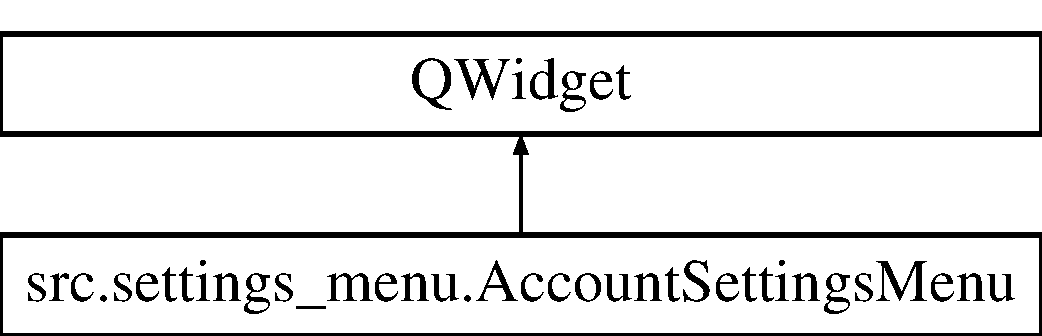
\includegraphics[height=2.000000cm]{classsrc_1_1settings__menu_1_1_account_settings_menu}
\end{center}
\end{figure}
\subsection*{Public Member Functions}
\begin{DoxyCompactItemize}
\item 
\hypertarget{classsrc_1_1settings__menu_1_1_account_settings_menu_a4b199df6972058b64e123acda02b72a5}{}def {\bfseries \+\_\+\+\_\+init\+\_\+\+\_\+} (self, \hyperlink{classsrc_1_1settings__menu_1_1_account_settings_menu_afe50b3829d1054937762620263272c4b}{parent}, \hyperlink{classsrc_1_1settings__menu_1_1_account_settings_menu_a54d0681d7b2c05bc084bf686a5e0cf41}{username})\label{classsrc_1_1settings__menu_1_1_account_settings_menu_a4b199df6972058b64e123acda02b72a5}

\item 
def \hyperlink{classsrc_1_1settings__menu_1_1_account_settings_menu_aeff3b2a6031f6dd312a66d0f161eeedb}{init\+U\+I} (self)
\begin{DoxyCompactList}\small\item\em This method initializes the G\+U\+I for the account settings menu. \end{DoxyCompactList}\item 
def \hyperlink{classsrc_1_1settings__menu_1_1_account_settings_menu_a10989536edbbe0db4fc03f2e5ccc8271}{change\+Settings} (self)
\begin{DoxyCompactList}\small\item\em This method is used to change the user\textquotesingle{}s name,username A\+N\+D password. \end{DoxyCompactList}\item 
def \hyperlink{classsrc_1_1settings__menu_1_1_account_settings_menu_a47dc6e6cb8a9ca5431a32ad73298ed81}{back\+To\+Main\+Menu} (self)
\begin{DoxyCompactList}\small\item\em This method emit back\+To\+Main\+Menu\+Signal when called. \end{DoxyCompactList}\end{DoxyCompactItemize}
\subsection*{Public Attributes}
\begin{DoxyCompactItemize}
\item 
\hyperlink{classsrc_1_1settings__menu_1_1_account_settings_menu_afe50b3829d1054937762620263272c4b}{parent}
\begin{DoxyCompactList}\small\item\em Instance of this class\textquotesingle{}s parent. \end{DoxyCompactList}\item 
\hyperlink{classsrc_1_1settings__menu_1_1_account_settings_menu_a793f0abcc421d4f7e51d6ff02e3e86ea}{db}
\begin{DoxyCompactList}\small\item\em Instance of the database. \end{DoxyCompactList}\item 
\hyperlink{classsrc_1_1settings__menu_1_1_account_settings_menu_a6f5f05b647982a9776c96ea5ca254068}{title}
\begin{DoxyCompactList}\small\item\em A Q\+Label which displays the titles of following fields. \end{DoxyCompactList}\item 
\hyperlink{classsrc_1_1settings__menu_1_1_account_settings_menu_a72d6db1fc6e6253916fec2090e8ff914}{your\+Name}
\begin{DoxyCompactList}\small\item\em This is a Q\+Line\+Edit which the user can use to enter his new real name. \end{DoxyCompactList}\item 
\hyperlink{classsrc_1_1settings__menu_1_1_account_settings_menu_a54d0681d7b2c05bc084bf686a5e0cf41}{username}
\begin{DoxyCompactList}\small\item\em This is a Q\+Line\+Edit which the user can use to enter his new username. \end{DoxyCompactList}\item 
\hyperlink{classsrc_1_1settings__menu_1_1_account_settings_menu_a11ded2b607c6b7e0b756eef17952b1f6}{password}
\begin{DoxyCompactList}\small\item\em This is a Q\+Line\+Edit which the user can use to enter his new password. \end{DoxyCompactList}\item 
\hyperlink{classsrc_1_1settings__menu_1_1_account_settings_menu_a6ad9267209290b0eaa3ef35191f81d82}{change\+Button}
\begin{DoxyCompactList}\small\item\em This is a buttton that calls \hyperlink{classsrc_1_1settings__menu_1_1_account_settings_menu_a10989536edbbe0db4fc03f2e5ccc8271}{change\+Settings()} when clicked. \end{DoxyCompactList}\item 
\hyperlink{classsrc_1_1settings__menu_1_1_account_settings_menu_a80552690cf6643721ebc00319289468a}{back\+Button}
\begin{DoxyCompactList}\small\item\em This is a button that calls \hyperlink{classsrc_1_1settings__menu_1_1_account_settings_menu_a47dc6e6cb8a9ca5431a32ad73298ed81}{back\+To\+Main\+Menu()} when clicked. \end{DoxyCompactList}\end{DoxyCompactItemize}
\subsection*{Static Public Attributes}
\begin{DoxyCompactItemize}
\item 
\hyperlink{classsrc_1_1settings__menu_1_1_account_settings_menu_a7cac3d6c4fd01c1d0c9e6cfcba8e8950}{logged\+Username} = None
\begin{DoxyCompactList}\small\item\em Instance of the currently active user\textquotesingle{}s username. \end{DoxyCompactList}\item 
tuple \hyperlink{classsrc_1_1settings__menu_1_1_account_settings_menu_a968b438c9430d659dcb90a23689127be}{back\+To\+Main\+Menu\+Signal} = Qt\+Core.\+pyqt\+Signal()
\begin{DoxyCompactList}\small\item\em Signal which will be used to return to the main menu. \end{DoxyCompactList}\end{DoxyCompactItemize}


\subsection{Detailed Description}
This class is a widget that displays the account settings menu. 

It includes buttons and fields that the user can interact with.~\newline
 

\subsection{Member Function Documentation}
\hypertarget{classsrc_1_1settings__menu_1_1_account_settings_menu_a47dc6e6cb8a9ca5431a32ad73298ed81}{}\index{src\+::settings\+\_\+menu\+::\+Account\+Settings\+Menu@{src\+::settings\+\_\+menu\+::\+Account\+Settings\+Menu}!back\+To\+Main\+Menu@{back\+To\+Main\+Menu}}
\index{back\+To\+Main\+Menu@{back\+To\+Main\+Menu}!src\+::settings\+\_\+menu\+::\+Account\+Settings\+Menu@{src\+::settings\+\_\+menu\+::\+Account\+Settings\+Menu}}
\subsubsection[{back\+To\+Main\+Menu}]{\setlength{\rightskip}{0pt plus 5cm}def src.\+settings\+\_\+menu.\+Account\+Settings\+Menu.\+back\+To\+Main\+Menu (
\begin{DoxyParamCaption}
\item[{}]{self}
\end{DoxyParamCaption}
)}\label{classsrc_1_1settings__menu_1_1_account_settings_menu_a47dc6e6cb8a9ca5431a32ad73298ed81}


This method emit back\+To\+Main\+Menu\+Signal when called. 

\hypertarget{classsrc_1_1settings__menu_1_1_account_settings_menu_a10989536edbbe0db4fc03f2e5ccc8271}{}\index{src\+::settings\+\_\+menu\+::\+Account\+Settings\+Menu@{src\+::settings\+\_\+menu\+::\+Account\+Settings\+Menu}!change\+Settings@{change\+Settings}}
\index{change\+Settings@{change\+Settings}!src\+::settings\+\_\+menu\+::\+Account\+Settings\+Menu@{src\+::settings\+\_\+menu\+::\+Account\+Settings\+Menu}}
\subsubsection[{change\+Settings}]{\setlength{\rightskip}{0pt plus 5cm}def src.\+settings\+\_\+menu.\+Account\+Settings\+Menu.\+change\+Settings (
\begin{DoxyParamCaption}
\item[{}]{self}
\end{DoxyParamCaption}
)}\label{classsrc_1_1settings__menu_1_1_account_settings_menu_a10989536edbbe0db4fc03f2e5ccc8271}


This method is used to change the user\textquotesingle{}s name,username A\+N\+D password. 

\hypertarget{classsrc_1_1settings__menu_1_1_account_settings_menu_aeff3b2a6031f6dd312a66d0f161eeedb}{}\index{src\+::settings\+\_\+menu\+::\+Account\+Settings\+Menu@{src\+::settings\+\_\+menu\+::\+Account\+Settings\+Menu}!init\+U\+I@{init\+U\+I}}
\index{init\+U\+I@{init\+U\+I}!src\+::settings\+\_\+menu\+::\+Account\+Settings\+Menu@{src\+::settings\+\_\+menu\+::\+Account\+Settings\+Menu}}
\subsubsection[{init\+U\+I}]{\setlength{\rightskip}{0pt plus 5cm}def src.\+settings\+\_\+menu.\+Account\+Settings\+Menu.\+init\+U\+I (
\begin{DoxyParamCaption}
\item[{}]{self}
\end{DoxyParamCaption}
)}\label{classsrc_1_1settings__menu_1_1_account_settings_menu_aeff3b2a6031f6dd312a66d0f161eeedb}


This method initializes the G\+U\+I for the account settings menu. 



\subsection{Member Data Documentation}
\hypertarget{classsrc_1_1settings__menu_1_1_account_settings_menu_a80552690cf6643721ebc00319289468a}{}\index{src\+::settings\+\_\+menu\+::\+Account\+Settings\+Menu@{src\+::settings\+\_\+menu\+::\+Account\+Settings\+Menu}!back\+Button@{back\+Button}}
\index{back\+Button@{back\+Button}!src\+::settings\+\_\+menu\+::\+Account\+Settings\+Menu@{src\+::settings\+\_\+menu\+::\+Account\+Settings\+Menu}}
\subsubsection[{back\+Button}]{\setlength{\rightskip}{0pt plus 5cm}src.\+settings\+\_\+menu.\+Account\+Settings\+Menu.\+back\+Button}\label{classsrc_1_1settings__menu_1_1_account_settings_menu_a80552690cf6643721ebc00319289468a}


This is a button that calls \hyperlink{classsrc_1_1settings__menu_1_1_account_settings_menu_a47dc6e6cb8a9ca5431a32ad73298ed81}{back\+To\+Main\+Menu()} when clicked. 

\hypertarget{classsrc_1_1settings__menu_1_1_account_settings_menu_a968b438c9430d659dcb90a23689127be}{}\index{src\+::settings\+\_\+menu\+::\+Account\+Settings\+Menu@{src\+::settings\+\_\+menu\+::\+Account\+Settings\+Menu}!back\+To\+Main\+Menu\+Signal@{back\+To\+Main\+Menu\+Signal}}
\index{back\+To\+Main\+Menu\+Signal@{back\+To\+Main\+Menu\+Signal}!src\+::settings\+\_\+menu\+::\+Account\+Settings\+Menu@{src\+::settings\+\_\+menu\+::\+Account\+Settings\+Menu}}
\subsubsection[{back\+To\+Main\+Menu\+Signal}]{\setlength{\rightskip}{0pt plus 5cm}tuple src.\+settings\+\_\+menu.\+Account\+Settings\+Menu.\+back\+To\+Main\+Menu\+Signal = Qt\+Core.\+pyqt\+Signal()\hspace{0.3cm}{\ttfamily [static]}}\label{classsrc_1_1settings__menu_1_1_account_settings_menu_a968b438c9430d659dcb90a23689127be}


Signal which will be used to return to the main menu. 

\hypertarget{classsrc_1_1settings__menu_1_1_account_settings_menu_a6ad9267209290b0eaa3ef35191f81d82}{}\index{src\+::settings\+\_\+menu\+::\+Account\+Settings\+Menu@{src\+::settings\+\_\+menu\+::\+Account\+Settings\+Menu}!change\+Button@{change\+Button}}
\index{change\+Button@{change\+Button}!src\+::settings\+\_\+menu\+::\+Account\+Settings\+Menu@{src\+::settings\+\_\+menu\+::\+Account\+Settings\+Menu}}
\subsubsection[{change\+Button}]{\setlength{\rightskip}{0pt plus 5cm}src.\+settings\+\_\+menu.\+Account\+Settings\+Menu.\+change\+Button}\label{classsrc_1_1settings__menu_1_1_account_settings_menu_a6ad9267209290b0eaa3ef35191f81d82}


This is a buttton that calls \hyperlink{classsrc_1_1settings__menu_1_1_account_settings_menu_a10989536edbbe0db4fc03f2e5ccc8271}{change\+Settings()} when clicked. 

\hypertarget{classsrc_1_1settings__menu_1_1_account_settings_menu_a793f0abcc421d4f7e51d6ff02e3e86ea}{}\index{src\+::settings\+\_\+menu\+::\+Account\+Settings\+Menu@{src\+::settings\+\_\+menu\+::\+Account\+Settings\+Menu}!db@{db}}
\index{db@{db}!src\+::settings\+\_\+menu\+::\+Account\+Settings\+Menu@{src\+::settings\+\_\+menu\+::\+Account\+Settings\+Menu}}
\subsubsection[{db}]{\setlength{\rightskip}{0pt plus 5cm}src.\+settings\+\_\+menu.\+Account\+Settings\+Menu.\+db}\label{classsrc_1_1settings__menu_1_1_account_settings_menu_a793f0abcc421d4f7e51d6ff02e3e86ea}


Instance of the database. 

\hypertarget{classsrc_1_1settings__menu_1_1_account_settings_menu_a7cac3d6c4fd01c1d0c9e6cfcba8e8950}{}\index{src\+::settings\+\_\+menu\+::\+Account\+Settings\+Menu@{src\+::settings\+\_\+menu\+::\+Account\+Settings\+Menu}!logged\+Username@{logged\+Username}}
\index{logged\+Username@{logged\+Username}!src\+::settings\+\_\+menu\+::\+Account\+Settings\+Menu@{src\+::settings\+\_\+menu\+::\+Account\+Settings\+Menu}}
\subsubsection[{logged\+Username}]{\setlength{\rightskip}{0pt plus 5cm}src.\+settings\+\_\+menu.\+Account\+Settings\+Menu.\+logged\+Username = None\hspace{0.3cm}{\ttfamily [static]}}\label{classsrc_1_1settings__menu_1_1_account_settings_menu_a7cac3d6c4fd01c1d0c9e6cfcba8e8950}


Instance of the currently active user\textquotesingle{}s username. 

\hypertarget{classsrc_1_1settings__menu_1_1_account_settings_menu_afe50b3829d1054937762620263272c4b}{}\index{src\+::settings\+\_\+menu\+::\+Account\+Settings\+Menu@{src\+::settings\+\_\+menu\+::\+Account\+Settings\+Menu}!parent@{parent}}
\index{parent@{parent}!src\+::settings\+\_\+menu\+::\+Account\+Settings\+Menu@{src\+::settings\+\_\+menu\+::\+Account\+Settings\+Menu}}
\subsubsection[{parent}]{\setlength{\rightskip}{0pt plus 5cm}src.\+settings\+\_\+menu.\+Account\+Settings\+Menu.\+parent}\label{classsrc_1_1settings__menu_1_1_account_settings_menu_afe50b3829d1054937762620263272c4b}


Instance of this class\textquotesingle{}s parent. 

\hypertarget{classsrc_1_1settings__menu_1_1_account_settings_menu_a11ded2b607c6b7e0b756eef17952b1f6}{}\index{src\+::settings\+\_\+menu\+::\+Account\+Settings\+Menu@{src\+::settings\+\_\+menu\+::\+Account\+Settings\+Menu}!password@{password}}
\index{password@{password}!src\+::settings\+\_\+menu\+::\+Account\+Settings\+Menu@{src\+::settings\+\_\+menu\+::\+Account\+Settings\+Menu}}
\subsubsection[{password}]{\setlength{\rightskip}{0pt plus 5cm}src.\+settings\+\_\+menu.\+Account\+Settings\+Menu.\+password}\label{classsrc_1_1settings__menu_1_1_account_settings_menu_a11ded2b607c6b7e0b756eef17952b1f6}


This is a Q\+Line\+Edit which the user can use to enter his new password. 

\hypertarget{classsrc_1_1settings__menu_1_1_account_settings_menu_a6f5f05b647982a9776c96ea5ca254068}{}\index{src\+::settings\+\_\+menu\+::\+Account\+Settings\+Menu@{src\+::settings\+\_\+menu\+::\+Account\+Settings\+Menu}!title@{title}}
\index{title@{title}!src\+::settings\+\_\+menu\+::\+Account\+Settings\+Menu@{src\+::settings\+\_\+menu\+::\+Account\+Settings\+Menu}}
\subsubsection[{title}]{\setlength{\rightskip}{0pt plus 5cm}src.\+settings\+\_\+menu.\+Account\+Settings\+Menu.\+title}\label{classsrc_1_1settings__menu_1_1_account_settings_menu_a6f5f05b647982a9776c96ea5ca254068}


A Q\+Label which displays the titles of following fields. 

\hypertarget{classsrc_1_1settings__menu_1_1_account_settings_menu_a54d0681d7b2c05bc084bf686a5e0cf41}{}\index{src\+::settings\+\_\+menu\+::\+Account\+Settings\+Menu@{src\+::settings\+\_\+menu\+::\+Account\+Settings\+Menu}!username@{username}}
\index{username@{username}!src\+::settings\+\_\+menu\+::\+Account\+Settings\+Menu@{src\+::settings\+\_\+menu\+::\+Account\+Settings\+Menu}}
\subsubsection[{username}]{\setlength{\rightskip}{0pt plus 5cm}src.\+settings\+\_\+menu.\+Account\+Settings\+Menu.\+username}\label{classsrc_1_1settings__menu_1_1_account_settings_menu_a54d0681d7b2c05bc084bf686a5e0cf41}


This is a Q\+Line\+Edit which the user can use to enter his new username. 

\hypertarget{classsrc_1_1settings__menu_1_1_account_settings_menu_a72d6db1fc6e6253916fec2090e8ff914}{}\index{src\+::settings\+\_\+menu\+::\+Account\+Settings\+Menu@{src\+::settings\+\_\+menu\+::\+Account\+Settings\+Menu}!your\+Name@{your\+Name}}
\index{your\+Name@{your\+Name}!src\+::settings\+\_\+menu\+::\+Account\+Settings\+Menu@{src\+::settings\+\_\+menu\+::\+Account\+Settings\+Menu}}
\subsubsection[{your\+Name}]{\setlength{\rightskip}{0pt plus 5cm}src.\+settings\+\_\+menu.\+Account\+Settings\+Menu.\+your\+Name}\label{classsrc_1_1settings__menu_1_1_account_settings_menu_a72d6db1fc6e6253916fec2090e8ff914}


This is a Q\+Line\+Edit which the user can use to enter his new real name. 



The documentation for this class was generated from the following file\+:\begin{DoxyCompactItemize}
\item 
src/settings\+\_\+menu.\+py\end{DoxyCompactItemize}

\hypertarget{classsrc_1_1board_1_1_board}{}\section{src.\+board.\+Board Class Reference}
\label{classsrc_1_1board_1_1_board}\index{src.\+board.\+Board@{src.\+board.\+Board}}


This class displays the board for the gameplay.  


Inheritance diagram for src.\+board.\+Board\+:\begin{figure}[H]
\begin{center}
\leavevmode
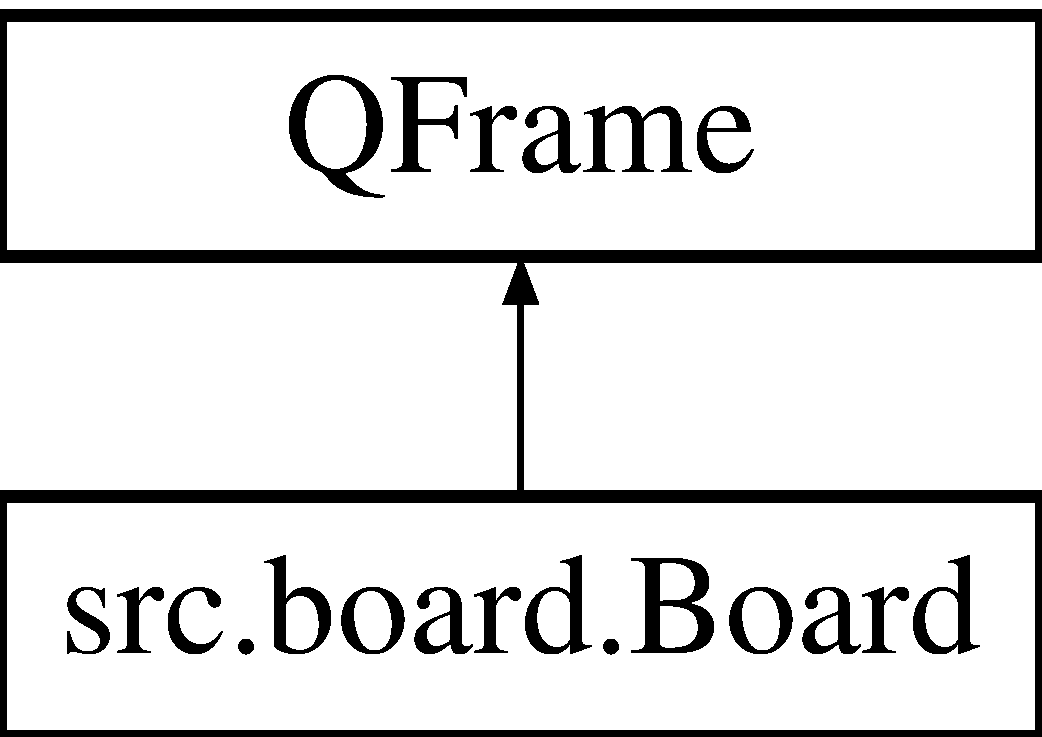
\includegraphics[height=2.000000cm]{classsrc_1_1board_1_1_board}
\end{center}
\end{figure}
\subsection*{Public Member Functions}
\begin{DoxyCompactItemize}
\item 
\hypertarget{classsrc_1_1board_1_1_board_ae8571472bb4178812dd941cf3f8e5f7c}{}def {\bfseries \+\_\+\+\_\+init\+\_\+\+\_\+}\label{classsrc_1_1board_1_1_board_ae8571472bb4178812dd941cf3f8e5f7c}

\item 
def \hyperlink{classsrc_1_1board_1_1_board_a9088e838b9bb196505af60eb1598495c}{init\+Status\+Bar} (self)
\begin{DoxyCompactList}\small\item\em This method initializes the status bar. \end{DoxyCompactList}\item 
def \hyperlink{classsrc_1_1board_1_1_board_a3ea0ac2d9356f9ebe6a63176b2351b5b}{init\+Board} (self)
\begin{DoxyCompactList}\small\item\em This method initializes the board. \end{DoxyCompactList}\item 
def \hyperlink{classsrc_1_1board_1_1_board_a2b87c8bc2da1173e07467996e4facbc4}{init\+Level} (self)
\begin{DoxyCompactList}\small\item\em This method initializes a new level. \end{DoxyCompactList}\item 
def \hyperlink{classsrc_1_1board_1_1_board_a97be76e6fb7312dddd9c86290fc3a1db}{start} (self)
\begin{DoxyCompactList}\small\item\em This method starts the board. \end{DoxyCompactList}\item 
def \hyperlink{classsrc_1_1board_1_1_board_a29473ffbf635f04428be1349d177eedc}{pause} (self)
\begin{DoxyCompactList}\small\item\em This method pauses the game. \end{DoxyCompactList}\item 
def \hyperlink{classsrc_1_1board_1_1_board_a68ece335899ccecebb6ecb39c339d180}{death} (self)
\begin{DoxyCompactList}\small\item\em This method takes care of bomberman\textquotesingle{}s death. \end{DoxyCompactList}\item 
def \hyperlink{classsrc_1_1board_1_1_board_afc740240caba216e9b416bdae675aab6}{tile\+At} (self, x, y)
\begin{DoxyCompactList}\small\item\em This method the tile which is at specific coordinates. \end{DoxyCompactList}\item 
def \hyperlink{classsrc_1_1board_1_1_board_ac40120a47f2787cb730e2d945e8833ee}{set\+Tile\+At} (self, x, y, tile)
\begin{DoxyCompactList}\small\item\em This method pushes a tile and then updates the board. \end{DoxyCompactList}\item 
def \hyperlink{classsrc_1_1board_1_1_board_a78d9960666f0be862cad75c855a38709}{set\+Tile\+At\+Without\+Update} (self, x, y, tile)
\begin{DoxyCompactList}\small\item\em This method pushes a tile without updating the board. \end{DoxyCompactList}\item 
def \hyperlink{classsrc_1_1board_1_1_board_af2e08aecc48abfbb38dfcc2dbc11b7cd}{pop\+Tile\+At} (self, x, y)
\begin{DoxyCompactList}\small\item\em This method pops a tile at coordinates x and y and then updates the board. \end{DoxyCompactList}\item 
def \hyperlink{classsrc_1_1board_1_1_board_a84399c357c601a4cf2f64dd096c2adc7}{pop\+Tile\+At\+Without\+Update} (self, x, y)
\begin{DoxyCompactList}\small\item\em This method pops a tile at coordinates x and y without updating the board. \end{DoxyCompactList}\item 
def \hyperlink{classsrc_1_1board_1_1_board_a4d2d336061f0136c40c42f491e11ad02}{square\+Width} (self)
\begin{DoxyCompactList}\small\item\em This method returns the width of a single tile. \end{DoxyCompactList}\item 
def \hyperlink{classsrc_1_1board_1_1_board_a1e964f3382db079501c6b4afa16348e4}{square\+Height} (self)
\begin{DoxyCompactList}\small\item\em This method returns the height of a single tile. \end{DoxyCompactList}\item 
\hypertarget{classsrc_1_1board_1_1_board_a7734f1ae8cb324abbafc0e1af7f4db6f}{}def {\bfseries bomb\+Loop} (self)\label{classsrc_1_1board_1_1_board_a7734f1ae8cb324abbafc0e1af7f4db6f}

\item 
def \hyperlink{classsrc_1_1board_1_1_board_aea8bc4036301719acbca3f62aa98e125}{paint\+Event} (self, event)
\begin{DoxyCompactList}\small\item\em This method is used to draw the board. \end{DoxyCompactList}\item 
def \hyperlink{classsrc_1_1board_1_1_board_ac85b9f4f5c9a91b200fb7e9e75d69d29}{draw\+Images} (self, painter, shape, x, y)
\begin{DoxyCompactList}\small\item\em This method draws the image to the board. \end{DoxyCompactList}\item 
def \hyperlink{classsrc_1_1board_1_1_board_a5e6978f5baf0f94e864867df77d5c891}{draw\+Square} (self, painter, x, y, shape)
\begin{DoxyCompactList}\small\item\em This method draws squares the represent Bricks, Concrete and Empty Tiles. \end{DoxyCompactList}\item 
def \hyperlink{classsrc_1_1board_1_1_board_a656fb42b7e9a4e4b5aae20c261170fe3}{key\+Press\+Event} (self, event)
\begin{DoxyCompactList}\small\item\em This method calls methods after keys are pressed. \end{DoxyCompactList}\item 
def \hyperlink{classsrc_1_1board_1_1_board_a663a599889dead3d876c4e4d79123b8e}{try\+Move} (self, new\+X, new\+Y)
\begin{DoxyCompactList}\small\item\em A method that moves bomberman one tile. \end{DoxyCompactList}\item 
def \hyperlink{classsrc_1_1board_1_1_board_abcf6e3affb8c4b83c6d0ab28e265b4d5}{move\+Enemy} (self, speed)
\begin{DoxyCompactList}\small\item\em Method that moves every enemy of a certain speed if able. \end{DoxyCompactList}\item 
def \hyperlink{classsrc_1_1board_1_1_board_a60ef4247af25957bcaaa0469eb222ac1}{bomberman\+Trigger\+Can\+Move} (self)
\begin{DoxyCompactList}\small\item\em Method that allows bomberman to move. \end{DoxyCompactList}\item 
def \hyperlink{classsrc_1_1board_1_1_board_a4e6bd40bde952bdbe12653269da596f5}{kill\+Enemy} (self, x, y)
\begin{DoxyCompactList}\small\item\em This method kills an enemy if it is at a given coordinate. \end{DoxyCompactList}\item 
def \hyperlink{classsrc_1_1board_1_1_board_a801979e5433ee99d7e36a4c648b3f930}{detonate\+Bomb} (self)
\begin{DoxyCompactList}\small\item\em This method detonates the first bomb in bomb\+Queue. \end{DoxyCompactList}\item 
def \hyperlink{classsrc_1_1board_1_1_board_a39006efbb358f5be11d11c3a2775a2f0}{start\+Flash} (self, flash\+List)
\begin{DoxyCompactList}\small\item\em This method changes every tile on the flash\+List to Tile.\+Flash  The list of tiles to be flashed. \end{DoxyCompactList}\item 
def \hyperlink{classsrc_1_1board_1_1_board_a1a709b1fbf97db6da5740b7aeac1fad8}{end\+Flash} (self, flash\+List)
\begin{DoxyCompactList}\small\item\em This method pops all Tile.\+Flash from the list flash\+List. \end{DoxyCompactList}\item 
def \hyperlink{classsrc_1_1board_1_1_board_a537d8c1c7d64aebc960da0f0b34ef44c}{destroy\+Tiles} (self, pop\+List)
\begin{DoxyCompactList}\small\item\em This method pops all the tiles on the pop\+List. \end{DoxyCompactList}\item 
def \hyperlink{classsrc_1_1board_1_1_board_a718f3d710ba5aa31fb49da72d37c450a}{exit} (self)
\begin{DoxyCompactList}\small\item\em This method stops timers and ends the game when the exit of level 16 is reached. \end{DoxyCompactList}\item 
def \hyperlink{classsrc_1_1board_1_1_board_a218749642f3aec8d8daaaf6be61cf0a9}{stop\+Timers} (self)
\begin{DoxyCompactList}\small\item\em This method stops all the timers. \end{DoxyCompactList}\item 
def \hyperlink{classsrc_1_1board_1_1_board_aa7b557053364da15e7a150537bf37757}{restart\+Next\+Level} (self)
\begin{DoxyCompactList}\small\item\em This method initialized a new next level. \end{DoxyCompactList}\item 
def \hyperlink{classsrc_1_1board_1_1_board_a962e440ddb9556ca233a686d3d9f1be0}{restart\+Same\+Level} (self)
\begin{DoxyCompactList}\small\item\em This method initializes a new same level. \end{DoxyCompactList}\item 
\hypertarget{classsrc_1_1board_1_1_board_a69b2b3031f0df523ba3dbeab4bfd3fb2}{}def \hyperlink{classsrc_1_1board_1_1_board_a69b2b3031f0df523ba3dbeab4bfd3fb2}{update\+Score} (self, killed\+Enemies)\label{classsrc_1_1board_1_1_board_a69b2b3031f0df523ba3dbeab4bfd3fb2}

\begin{DoxyCompactList}\small\item\em This method updates the score in status bar. \end{DoxyCompactList}\item 
def \hyperlink{classsrc_1_1board_1_1_board_a6a27183b76d873505d619fc6b78935b9}{get\+Score\+Of\+Killed\+Enemies} (self, killed\+Enemies)
\begin{DoxyCompactList}\small\item\em Method to calculate the score the user gets when a bomb detonates. \end{DoxyCompactList}\item 
def \hyperlink{classsrc_1_1board_1_1_board_a1320cdff86fe637b41b8973cf6bcb499}{save\+Bomberman} (self)
\begin{DoxyCompactList}\small\item\em This method returns the level. \end{DoxyCompactList}\item 
def \hyperlink{classsrc_1_1board_1_1_board_afa56e069dac6b7cdc60ba45e91d1745c}{timeout\+Event} (self)
\begin{DoxyCompactList}\small\item\em This method decreses the time by 1 until the time is 0. \end{DoxyCompactList}\end{DoxyCompactItemize}
\subsection*{Public Attributes}
\begin{DoxyCompactItemize}
\item 
\hypertarget{classsrc_1_1board_1_1_board_a553447e81840fb800b7ab2f74702ccfb}{}{\bfseries level}\label{classsrc_1_1board_1_1_board_a553447e81840fb800b7ab2f74702ccfb}

\item 
\hypertarget{classsrc_1_1board_1_1_board_a5b5a2ac1a742155264df3668a470335f}{}{\bfseries status\+Bar}\label{classsrc_1_1board_1_1_board_a5b5a2ac1a742155264df3668a470335f}

\item 
\hypertarget{classsrc_1_1board_1_1_board_a0b508a29cd8fed07fcb8cc9ab0c3fc0d}{}{\bfseries is\+Paused}\label{classsrc_1_1board_1_1_board_a0b508a29cd8fed07fcb8cc9ab0c3fc0d}

\item 
\hypertarget{classsrc_1_1board_1_1_board_a693000531a35e8c699aa56262ed6d10a}{}{\bfseries global\+Timer}\label{classsrc_1_1board_1_1_board_a693000531a35e8c699aa56262ed6d10a}

\item 
\hypertarget{classsrc_1_1board_1_1_board_ac8c6d710d39e770a99356a30cabf275b}{}{\bfseries fast\+Timer}\label{classsrc_1_1board_1_1_board_ac8c6d710d39e770a99356a30cabf275b}

\item 
\hypertarget{classsrc_1_1board_1_1_board_a18fce871d4c91bac16992dbd2975ebda}{}{\bfseries normal\+Timer}\label{classsrc_1_1board_1_1_board_a18fce871d4c91bac16992dbd2975ebda}

\item 
\hypertarget{classsrc_1_1board_1_1_board_af0477a0dda0a5b27f4f931f89da25180}{}{\bfseries slow\+Timer}\label{classsrc_1_1board_1_1_board_af0477a0dda0a5b27f4f931f89da25180}

\item 
\hypertarget{classsrc_1_1board_1_1_board_ab11b4588420cef13c3d035a2607362d0}{}{\bfseries slowest\+Timer}\label{classsrc_1_1board_1_1_board_ab11b4588420cef13c3d035a2607362d0}

\item 
\hypertarget{classsrc_1_1board_1_1_board_a91635719cb9bc632fa29a4185b1ffaa4}{}{\bfseries coundown\+Timer}\label{classsrc_1_1board_1_1_board_a91635719cb9bc632fa29a4185b1ffaa4}

\end{DoxyCompactItemize}
\subsection*{Static Public Attributes}
\begin{DoxyCompactItemize}
\item 
\hypertarget{classsrc_1_1board_1_1_board_a3d20eac8eee8f73f9fd84ca14a9a99d5}{}tuple {\bfseries pause\+Game\+Signal} = Qt\+Core.\+pyqt\+Signal()\label{classsrc_1_1board_1_1_board_a3d20eac8eee8f73f9fd84ca14a9a99d5}

\item 
\hypertarget{classsrc_1_1board_1_1_board_a88d390d2d4ad6a255712abdde9f737e0}{}tuple {\bfseries game\+Over\+Signal} = Qt\+Core.\+pyqt\+Signal()\label{classsrc_1_1board_1_1_board_a88d390d2d4ad6a255712abdde9f737e0}

\item 
\hypertarget{classsrc_1_1board_1_1_board_afbf20580188f637d8d5863a9a9810ff5}{}tuple {\bfseries reset\+Timer\+Signal} = Qt\+Core.\+pyqt\+Signal()\label{classsrc_1_1board_1_1_board_afbf20580188f637d8d5863a9a9810ff5}

\item 
\hypertarget{classsrc_1_1board_1_1_board_adbdb04e00742a09c938f8cb3f751e1f9}{}tuple {\bfseries update\+Score\+In\+Db\+Signal} = Qt\+Core.\+pyqt\+Signal(int)\label{classsrc_1_1board_1_1_board_adbdb04e00742a09c938f8cb3f751e1f9}

\end{DoxyCompactItemize}


\subsection{Detailed Description}
This class displays the board for the gameplay. 

It handles drawing each tile. It also contains timers and methods that allow movement of bomberman and enemies. 

\subsection{Member Function Documentation}
\hypertarget{classsrc_1_1board_1_1_board_a60ef4247af25957bcaaa0469eb222ac1}{}\index{src\+::board\+::\+Board@{src\+::board\+::\+Board}!bomberman\+Trigger\+Can\+Move@{bomberman\+Trigger\+Can\+Move}}
\index{bomberman\+Trigger\+Can\+Move@{bomberman\+Trigger\+Can\+Move}!src\+::board\+::\+Board@{src\+::board\+::\+Board}}
\subsubsection[{bomberman\+Trigger\+Can\+Move}]{\setlength{\rightskip}{0pt plus 5cm}def src.\+board.\+Board.\+bomberman\+Trigger\+Can\+Move (
\begin{DoxyParamCaption}
\item[{}]{self}
\end{DoxyParamCaption}
)}\label{classsrc_1_1board_1_1_board_a60ef4247af25957bcaaa0469eb222ac1}


Method that allows bomberman to move. 

Triggers after a set amount of time. \hypertarget{classsrc_1_1board_1_1_board_a68ece335899ccecebb6ecb39c339d180}{}\index{src\+::board\+::\+Board@{src\+::board\+::\+Board}!death@{death}}
\index{death@{death}!src\+::board\+::\+Board@{src\+::board\+::\+Board}}
\subsubsection[{death}]{\setlength{\rightskip}{0pt plus 5cm}def src.\+board.\+Board.\+death (
\begin{DoxyParamCaption}
\item[{}]{self}
\end{DoxyParamCaption}
)}\label{classsrc_1_1board_1_1_board_a68ece335899ccecebb6ecb39c339d180}


This method takes care of bomberman\textquotesingle{}s death. 

It stops the timers and removes a life. If lives equals 0 then it ends the game. If not, it reinitializes the current level. \hypertarget{classsrc_1_1board_1_1_board_a537d8c1c7d64aebc960da0f0b34ef44c}{}\index{src\+::board\+::\+Board@{src\+::board\+::\+Board}!destroy\+Tiles@{destroy\+Tiles}}
\index{destroy\+Tiles@{destroy\+Tiles}!src\+::board\+::\+Board@{src\+::board\+::\+Board}}
\subsubsection[{destroy\+Tiles}]{\setlength{\rightskip}{0pt plus 5cm}def src.\+board.\+Board.\+destroy\+Tiles (
\begin{DoxyParamCaption}
\item[{}]{self, }
\item[{}]{pop\+List}
\end{DoxyParamCaption}
)}\label{classsrc_1_1board_1_1_board_a537d8c1c7d64aebc960da0f0b34ef44c}


This method pops all the tiles on the pop\+List. 

pop\+List The list of tiles to be popped. \hypertarget{classsrc_1_1board_1_1_board_a801979e5433ee99d7e36a4c648b3f930}{}\index{src\+::board\+::\+Board@{src\+::board\+::\+Board}!detonate\+Bomb@{detonate\+Bomb}}
\index{detonate\+Bomb@{detonate\+Bomb}!src\+::board\+::\+Board@{src\+::board\+::\+Board}}
\subsubsection[{detonate\+Bomb}]{\setlength{\rightskip}{0pt plus 5cm}def src.\+board.\+Board.\+detonate\+Bomb (
\begin{DoxyParamCaption}
\item[{}]{self}
\end{DoxyParamCaption}
)}\label{classsrc_1_1board_1_1_board_a801979e5433ee99d7e36a4c648b3f930}


This method detonates the first bomb in bomb\+Queue. 

flash\+List is a list of tiles that are turned orange after the bomb is detonated. pop\+List is a list of tiles to be popped. killed\+Enemies is a list of tiles where enemies are to be killed. This method checks the four cardinal directions from the bomb for bricks that aren\textquotesingle{}t empty or concrete and acts according to the tile type. \hypertarget{classsrc_1_1board_1_1_board_ac85b9f4f5c9a91b200fb7e9e75d69d29}{}\index{src\+::board\+::\+Board@{src\+::board\+::\+Board}!draw\+Images@{draw\+Images}}
\index{draw\+Images@{draw\+Images}!src\+::board\+::\+Board@{src\+::board\+::\+Board}}
\subsubsection[{draw\+Images}]{\setlength{\rightskip}{0pt plus 5cm}def src.\+board.\+Board.\+draw\+Images (
\begin{DoxyParamCaption}
\item[{}]{self, }
\item[{}]{painter, }
\item[{}]{shape, }
\item[{}]{x, }
\item[{}]{y}
\end{DoxyParamCaption}
)}\label{classsrc_1_1board_1_1_board_ac85b9f4f5c9a91b200fb7e9e75d69d29}


This method draws the image to the board. 

painter  shape The picture that is to be drawn.  x The x coordinate of the drawing.  y The y coordinate of the drawing. \hypertarget{classsrc_1_1board_1_1_board_a5e6978f5baf0f94e864867df77d5c891}{}\index{src\+::board\+::\+Board@{src\+::board\+::\+Board}!draw\+Square@{draw\+Square}}
\index{draw\+Square@{draw\+Square}!src\+::board\+::\+Board@{src\+::board\+::\+Board}}
\subsubsection[{draw\+Square}]{\setlength{\rightskip}{0pt plus 5cm}def src.\+board.\+Board.\+draw\+Square (
\begin{DoxyParamCaption}
\item[{}]{self, }
\item[{}]{painter, }
\item[{}]{x, }
\item[{}]{y, }
\item[{}]{shape}
\end{DoxyParamCaption}
)}\label{classsrc_1_1board_1_1_board_a5e6978f5baf0f94e864867df77d5c891}


This method draws squares the represent Bricks, Concrete and Empty Tiles. 

painter  shape The picture that is to be drawn.  x The x coordinate of the drawing.  y The y coordinate of the drawing. \hypertarget{classsrc_1_1board_1_1_board_a1a709b1fbf97db6da5740b7aeac1fad8}{}\index{src\+::board\+::\+Board@{src\+::board\+::\+Board}!end\+Flash@{end\+Flash}}
\index{end\+Flash@{end\+Flash}!src\+::board\+::\+Board@{src\+::board\+::\+Board}}
\subsubsection[{end\+Flash}]{\setlength{\rightskip}{0pt plus 5cm}def src.\+board.\+Board.\+end\+Flash (
\begin{DoxyParamCaption}
\item[{}]{self, }
\item[{}]{flash\+List}
\end{DoxyParamCaption}
)}\label{classsrc_1_1board_1_1_board_a1a709b1fbf97db6da5740b7aeac1fad8}


This method pops all Tile.\+Flash from the list flash\+List. 

flash\+List The list of tiles to be popped. \hypertarget{classsrc_1_1board_1_1_board_a718f3d710ba5aa31fb49da72d37c450a}{}\index{src\+::board\+::\+Board@{src\+::board\+::\+Board}!exit@{exit}}
\index{exit@{exit}!src\+::board\+::\+Board@{src\+::board\+::\+Board}}
\subsubsection[{exit}]{\setlength{\rightskip}{0pt plus 5cm}def src.\+board.\+Board.\+exit (
\begin{DoxyParamCaption}
\item[{}]{self}
\end{DoxyParamCaption}
)}\label{classsrc_1_1board_1_1_board_a718f3d710ba5aa31fb49da72d37c450a}


This method stops timers and ends the game when the exit of level 16 is reached. 

\hypertarget{classsrc_1_1board_1_1_board_a6a27183b76d873505d619fc6b78935b9}{}\index{src\+::board\+::\+Board@{src\+::board\+::\+Board}!get\+Score\+Of\+Killed\+Enemies@{get\+Score\+Of\+Killed\+Enemies}}
\index{get\+Score\+Of\+Killed\+Enemies@{get\+Score\+Of\+Killed\+Enemies}!src\+::board\+::\+Board@{src\+::board\+::\+Board}}
\subsubsection[{get\+Score\+Of\+Killed\+Enemies}]{\setlength{\rightskip}{0pt plus 5cm}def src.\+board.\+Board.\+get\+Score\+Of\+Killed\+Enemies (
\begin{DoxyParamCaption}
\item[{}]{self, }
\item[{}]{killed\+Enemies}
\end{DoxyParamCaption}
)}\label{classsrc_1_1board_1_1_board_a6a27183b76d873505d619fc6b78935b9}


Method to calculate the score the user gets when a bomb detonates. 


\begin{DoxyParams}{Parameters}
{\em killed\+Enemies} & Assume the list \char`\"{}killed\+Enemies\char`\"{} has the following format\+: \mbox{[}\mbox{[}enemies at distance = 1 from bomb\mbox{]}, \mbox{[}enemies at distance = 2 from bomb\mbox{]}, ... , \mbox{[}enemies at distance = range from bomb\mbox{]}\mbox{]} e.\+g.\+: \mbox{[}\mbox{[}Tile.\+Balloom, Tile.\+Oneal\mbox{]}, \mbox{[}\mbox{]}, \mbox{[}Tile.\+Doll\mbox{]}\mbox{]} means when the bomb exploded, there was a Balloom and an Oneal at distance 1, nothing at distance 2, and a Doll at distance 3 from the bomb. \\
\hline
\end{DoxyParams}
\hypertarget{classsrc_1_1board_1_1_board_a3ea0ac2d9356f9ebe6a63176b2351b5b}{}\index{src\+::board\+::\+Board@{src\+::board\+::\+Board}!init\+Board@{init\+Board}}
\index{init\+Board@{init\+Board}!src\+::board\+::\+Board@{src\+::board\+::\+Board}}
\subsubsection[{init\+Board}]{\setlength{\rightskip}{0pt plus 5cm}def src.\+board.\+Board.\+init\+Board (
\begin{DoxyParamCaption}
\item[{}]{self}
\end{DoxyParamCaption}
)}\label{classsrc_1_1board_1_1_board_a3ea0ac2d9356f9ebe6a63176b2351b5b}


This method initializes the board. 

It initializes the timers too. \hypertarget{classsrc_1_1board_1_1_board_a2b87c8bc2da1173e07467996e4facbc4}{}\index{src\+::board\+::\+Board@{src\+::board\+::\+Board}!init\+Level@{init\+Level}}
\index{init\+Level@{init\+Level}!src\+::board\+::\+Board@{src\+::board\+::\+Board}}
\subsubsection[{init\+Level}]{\setlength{\rightskip}{0pt plus 5cm}def src.\+board.\+Board.\+init\+Level (
\begin{DoxyParamCaption}
\item[{}]{self}
\end{DoxyParamCaption}
)}\label{classsrc_1_1board_1_1_board_a2b87c8bc2da1173e07467996e4facbc4}


This method initializes a new level. 

\hypertarget{classsrc_1_1board_1_1_board_a9088e838b9bb196505af60eb1598495c}{}\index{src\+::board\+::\+Board@{src\+::board\+::\+Board}!init\+Status\+Bar@{init\+Status\+Bar}}
\index{init\+Status\+Bar@{init\+Status\+Bar}!src\+::board\+::\+Board@{src\+::board\+::\+Board}}
\subsubsection[{init\+Status\+Bar}]{\setlength{\rightskip}{0pt plus 5cm}def src.\+board.\+Board.\+init\+Status\+Bar (
\begin{DoxyParamCaption}
\item[{}]{self}
\end{DoxyParamCaption}
)}\label{classsrc_1_1board_1_1_board_a9088e838b9bb196505af60eb1598495c}


This method initializes the status bar. 

\hypertarget{classsrc_1_1board_1_1_board_a656fb42b7e9a4e4b5aae20c261170fe3}{}\index{src\+::board\+::\+Board@{src\+::board\+::\+Board}!key\+Press\+Event@{key\+Press\+Event}}
\index{key\+Press\+Event@{key\+Press\+Event}!src\+::board\+::\+Board@{src\+::board\+::\+Board}}
\subsubsection[{key\+Press\+Event}]{\setlength{\rightskip}{0pt plus 5cm}def src.\+board.\+Board.\+key\+Press\+Event (
\begin{DoxyParamCaption}
\item[{}]{self, }
\item[{}]{event}
\end{DoxyParamCaption}
)}\label{classsrc_1_1board_1_1_board_a656fb42b7e9a4e4b5aae20c261170fe3}


This method calls methods after keys are pressed. 


\begin{DoxyParams}{Parameters}
{\em event} & The key that has been pressed~\newline
 P\+: self.\+pause() is called if pause menu isn\textquotesingle{}t open.~\newline
 Arrow keys\+: \hyperlink{classsrc_1_1board_1_1_board_a663a599889dead3d876c4e4d79123b8e}{try\+Move()} is called.~\newline
 Space or Z\+: set\+Bomb() is called.~\newline
 X or B\+: \hyperlink{classsrc_1_1board_1_1_board_a801979e5433ee99d7e36a4c648b3f930}{detonate\+Bomb()} is called. \\
\hline
\end{DoxyParams}
\hypertarget{classsrc_1_1board_1_1_board_a4e6bd40bde952bdbe12653269da596f5}{}\index{src\+::board\+::\+Board@{src\+::board\+::\+Board}!kill\+Enemy@{kill\+Enemy}}
\index{kill\+Enemy@{kill\+Enemy}!src\+::board\+::\+Board@{src\+::board\+::\+Board}}
\subsubsection[{kill\+Enemy}]{\setlength{\rightskip}{0pt plus 5cm}def src.\+board.\+Board.\+kill\+Enemy (
\begin{DoxyParamCaption}
\item[{}]{self, }
\item[{}]{x, }
\item[{}]{y}
\end{DoxyParamCaption}
)}\label{classsrc_1_1board_1_1_board_a4e6bd40bde952bdbe12653269da596f5}


This method kills an enemy if it is at a given coordinate. 


\begin{DoxyParams}{Parameters}
{\em x} & The x coordinate \\
\hline
{\em y} & The y coordinate This method checks to see if there is an enemy at a given coordinate and if there is, it pops the tile that the enemy is at, removes it from list\+Enemies, and decrements both number of enemies and list\+Type\+Enemies. \\
\hline
\end{DoxyParams}
\hypertarget{classsrc_1_1board_1_1_board_abcf6e3affb8c4b83c6d0ab28e265b4d5}{}\index{src\+::board\+::\+Board@{src\+::board\+::\+Board}!move\+Enemy@{move\+Enemy}}
\index{move\+Enemy@{move\+Enemy}!src\+::board\+::\+Board@{src\+::board\+::\+Board}}
\subsubsection[{move\+Enemy}]{\setlength{\rightskip}{0pt plus 5cm}def src.\+board.\+Board.\+move\+Enemy (
\begin{DoxyParamCaption}
\item[{}]{self, }
\item[{}]{speed}
\end{DoxyParamCaption}
)}\label{classsrc_1_1board_1_1_board_abcf6e3affb8c4b83c6d0ab28e265b4d5}


Method that moves every enemy of a certain speed if able. 


\begin{DoxyParams}{Parameters}
{\em speed} & The speed of the enemies that will be moving. Each enemy on the map is checked to see if their speed is equal to the speed that is passed. If the intelligence of the enemy is 2 or 3 then the 4 adjacent tiles are checked to see if bomberman is on them. If yes, the enemy moves onto bomberman. If no, there is a chance based on the intelligence level of the enemy that it changes direction. The enemy will reverse its direction is there is an obstacle in its path. If there is no obstacle in front of the enemy it moves forward one tile. \\
\hline
\end{DoxyParams}
\hypertarget{classsrc_1_1board_1_1_board_aea8bc4036301719acbca3f62aa98e125}{}\index{src\+::board\+::\+Board@{src\+::board\+::\+Board}!paint\+Event@{paint\+Event}}
\index{paint\+Event@{paint\+Event}!src\+::board\+::\+Board@{src\+::board\+::\+Board}}
\subsubsection[{paint\+Event}]{\setlength{\rightskip}{0pt plus 5cm}def src.\+board.\+Board.\+paint\+Event (
\begin{DoxyParamCaption}
\item[{}]{self, }
\item[{}]{event}
\end{DoxyParamCaption}
)}\label{classsrc_1_1board_1_1_board_aea8bc4036301719acbca3f62aa98e125}


This method is used to draw the board. 

event This method uses bomberman\textquotesingle{}s x position to decide what part of the board to draw. It then draws each square in the visible portion of the board. \hypertarget{classsrc_1_1board_1_1_board_a29473ffbf635f04428be1349d177eedc}{}\index{src\+::board\+::\+Board@{src\+::board\+::\+Board}!pause@{pause}}
\index{pause@{pause}!src\+::board\+::\+Board@{src\+::board\+::\+Board}}
\subsubsection[{pause}]{\setlength{\rightskip}{0pt plus 5cm}def src.\+board.\+Board.\+pause (
\begin{DoxyParamCaption}
\item[{}]{self}
\end{DoxyParamCaption}
)}\label{classsrc_1_1board_1_1_board_a29473ffbf635f04428be1349d177eedc}


This method pauses the game. 

It stops the timers and sends a signal to open the pause\+Menu. \hypertarget{classsrc_1_1board_1_1_board_af2e08aecc48abfbb38dfcc2dbc11b7cd}{}\index{src\+::board\+::\+Board@{src\+::board\+::\+Board}!pop\+Tile\+At@{pop\+Tile\+At}}
\index{pop\+Tile\+At@{pop\+Tile\+At}!src\+::board\+::\+Board@{src\+::board\+::\+Board}}
\subsubsection[{pop\+Tile\+At}]{\setlength{\rightskip}{0pt plus 5cm}def src.\+board.\+Board.\+pop\+Tile\+At (
\begin{DoxyParamCaption}
\item[{}]{self, }
\item[{}]{x, }
\item[{}]{y}
\end{DoxyParamCaption}
)}\label{classsrc_1_1board_1_1_board_af2e08aecc48abfbb38dfcc2dbc11b7cd}


This method pops a tile at coordinates x and y and then updates the board. 

x The x coordinate to be popped.  y The y coordinate to be popped. \hypertarget{classsrc_1_1board_1_1_board_a84399c357c601a4cf2f64dd096c2adc7}{}\index{src\+::board\+::\+Board@{src\+::board\+::\+Board}!pop\+Tile\+At\+Without\+Update@{pop\+Tile\+At\+Without\+Update}}
\index{pop\+Tile\+At\+Without\+Update@{pop\+Tile\+At\+Without\+Update}!src\+::board\+::\+Board@{src\+::board\+::\+Board}}
\subsubsection[{pop\+Tile\+At\+Without\+Update}]{\setlength{\rightskip}{0pt plus 5cm}def src.\+board.\+Board.\+pop\+Tile\+At\+Without\+Update (
\begin{DoxyParamCaption}
\item[{}]{self, }
\item[{}]{x, }
\item[{}]{y}
\end{DoxyParamCaption}
)}\label{classsrc_1_1board_1_1_board_a84399c357c601a4cf2f64dd096c2adc7}


This method pops a tile at coordinates x and y without updating the board. 

x The x coordinate to be popped.  y The y coordinate to be popped. \hypertarget{classsrc_1_1board_1_1_board_aa7b557053364da15e7a150537bf37757}{}\index{src\+::board\+::\+Board@{src\+::board\+::\+Board}!restart\+Next\+Level@{restart\+Next\+Level}}
\index{restart\+Next\+Level@{restart\+Next\+Level}!src\+::board\+::\+Board@{src\+::board\+::\+Board}}
\subsubsection[{restart\+Next\+Level}]{\setlength{\rightskip}{0pt plus 5cm}def src.\+board.\+Board.\+restart\+Next\+Level (
\begin{DoxyParamCaption}
\item[{}]{self}
\end{DoxyParamCaption}
)}\label{classsrc_1_1board_1_1_board_aa7b557053364da15e7a150537bf37757}


This method initialized a new next level. 

\hypertarget{classsrc_1_1board_1_1_board_a962e440ddb9556ca233a686d3d9f1be0}{}\index{src\+::board\+::\+Board@{src\+::board\+::\+Board}!restart\+Same\+Level@{restart\+Same\+Level}}
\index{restart\+Same\+Level@{restart\+Same\+Level}!src\+::board\+::\+Board@{src\+::board\+::\+Board}}
\subsubsection[{restart\+Same\+Level}]{\setlength{\rightskip}{0pt plus 5cm}def src.\+board.\+Board.\+restart\+Same\+Level (
\begin{DoxyParamCaption}
\item[{}]{self}
\end{DoxyParamCaption}
)}\label{classsrc_1_1board_1_1_board_a962e440ddb9556ca233a686d3d9f1be0}


This method initializes a new same level. 

\hypertarget{classsrc_1_1board_1_1_board_a1320cdff86fe637b41b8973cf6bcb499}{}\index{src\+::board\+::\+Board@{src\+::board\+::\+Board}!save\+Bomberman@{save\+Bomberman}}
\index{save\+Bomberman@{save\+Bomberman}!src\+::board\+::\+Board@{src\+::board\+::\+Board}}
\subsubsection[{save\+Bomberman}]{\setlength{\rightskip}{0pt plus 5cm}def src.\+board.\+Board.\+save\+Bomberman (
\begin{DoxyParamCaption}
\item[{}]{self}
\end{DoxyParamCaption}
)}\label{classsrc_1_1board_1_1_board_a1320cdff86fe637b41b8973cf6bcb499}


This method returns the level. 

\hypertarget{classsrc_1_1board_1_1_board_ac40120a47f2787cb730e2d945e8833ee}{}\index{src\+::board\+::\+Board@{src\+::board\+::\+Board}!set\+Tile\+At@{set\+Tile\+At}}
\index{set\+Tile\+At@{set\+Tile\+At}!src\+::board\+::\+Board@{src\+::board\+::\+Board}}
\subsubsection[{set\+Tile\+At}]{\setlength{\rightskip}{0pt plus 5cm}def src.\+board.\+Board.\+set\+Tile\+At (
\begin{DoxyParamCaption}
\item[{}]{self, }
\item[{}]{x, }
\item[{}]{y, }
\item[{}]{tile}
\end{DoxyParamCaption}
)}\label{classsrc_1_1board_1_1_board_ac40120a47f2787cb730e2d945e8833ee}


This method pushes a tile and then updates the board. 

x The x coordinate to be popped.  y The y coordinate to be popped.  tile The tile that is to be pushed. \hypertarget{classsrc_1_1board_1_1_board_a78d9960666f0be862cad75c855a38709}{}\index{src\+::board\+::\+Board@{src\+::board\+::\+Board}!set\+Tile\+At\+Without\+Update@{set\+Tile\+At\+Without\+Update}}
\index{set\+Tile\+At\+Without\+Update@{set\+Tile\+At\+Without\+Update}!src\+::board\+::\+Board@{src\+::board\+::\+Board}}
\subsubsection[{set\+Tile\+At\+Without\+Update}]{\setlength{\rightskip}{0pt plus 5cm}def src.\+board.\+Board.\+set\+Tile\+At\+Without\+Update (
\begin{DoxyParamCaption}
\item[{}]{self, }
\item[{}]{x, }
\item[{}]{y, }
\item[{}]{tile}
\end{DoxyParamCaption}
)}\label{classsrc_1_1board_1_1_board_a78d9960666f0be862cad75c855a38709}


This method pushes a tile without updating the board. 

x The x coordinate to be popped.  y The y coordinate to be popped.  tile The tile that is to be pushed. \hypertarget{classsrc_1_1board_1_1_board_a1e964f3382db079501c6b4afa16348e4}{}\index{src\+::board\+::\+Board@{src\+::board\+::\+Board}!square\+Height@{square\+Height}}
\index{square\+Height@{square\+Height}!src\+::board\+::\+Board@{src\+::board\+::\+Board}}
\subsubsection[{square\+Height}]{\setlength{\rightskip}{0pt plus 5cm}def src.\+board.\+Board.\+square\+Height (
\begin{DoxyParamCaption}
\item[{}]{self}
\end{DoxyParamCaption}
)}\label{classsrc_1_1board_1_1_board_a1e964f3382db079501c6b4afa16348e4}


This method returns the height of a single tile. 

\hypertarget{classsrc_1_1board_1_1_board_a4d2d336061f0136c40c42f491e11ad02}{}\index{src\+::board\+::\+Board@{src\+::board\+::\+Board}!square\+Width@{square\+Width}}
\index{square\+Width@{square\+Width}!src\+::board\+::\+Board@{src\+::board\+::\+Board}}
\subsubsection[{square\+Width}]{\setlength{\rightskip}{0pt plus 5cm}def src.\+board.\+Board.\+square\+Width (
\begin{DoxyParamCaption}
\item[{}]{self}
\end{DoxyParamCaption}
)}\label{classsrc_1_1board_1_1_board_a4d2d336061f0136c40c42f491e11ad02}


This method returns the width of a single tile. 

\hypertarget{classsrc_1_1board_1_1_board_a97be76e6fb7312dddd9c86290fc3a1db}{}\index{src\+::board\+::\+Board@{src\+::board\+::\+Board}!start@{start}}
\index{start@{start}!src\+::board\+::\+Board@{src\+::board\+::\+Board}}
\subsubsection[{start}]{\setlength{\rightskip}{0pt plus 5cm}def src.\+board.\+Board.\+start (
\begin{DoxyParamCaption}
\item[{}]{self}
\end{DoxyParamCaption}
)}\label{classsrc_1_1board_1_1_board_a97be76e6fb7312dddd9c86290fc3a1db}


This method starts the board. 

It sets is\+Paused to false and allows bomberman to begin moving. It also starts all the timers. \hypertarget{classsrc_1_1board_1_1_board_a39006efbb358f5be11d11c3a2775a2f0}{}\index{src\+::board\+::\+Board@{src\+::board\+::\+Board}!start\+Flash@{start\+Flash}}
\index{start\+Flash@{start\+Flash}!src\+::board\+::\+Board@{src\+::board\+::\+Board}}
\subsubsection[{start\+Flash}]{\setlength{\rightskip}{0pt plus 5cm}def src.\+board.\+Board.\+start\+Flash (
\begin{DoxyParamCaption}
\item[{}]{self, }
\item[{}]{flash\+List}
\end{DoxyParamCaption}
)}\label{classsrc_1_1board_1_1_board_a39006efbb358f5be11d11c3a2775a2f0}


This method changes every tile on the flash\+List to Tile.\+Flash  The list of tiles to be flashed. 

\hypertarget{classsrc_1_1board_1_1_board_a218749642f3aec8d8daaaf6be61cf0a9}{}\index{src\+::board\+::\+Board@{src\+::board\+::\+Board}!stop\+Timers@{stop\+Timers}}
\index{stop\+Timers@{stop\+Timers}!src\+::board\+::\+Board@{src\+::board\+::\+Board}}
\subsubsection[{stop\+Timers}]{\setlength{\rightskip}{0pt plus 5cm}def src.\+board.\+Board.\+stop\+Timers (
\begin{DoxyParamCaption}
\item[{}]{self}
\end{DoxyParamCaption}
)}\label{classsrc_1_1board_1_1_board_a218749642f3aec8d8daaaf6be61cf0a9}


This method stops all the timers. 

\hypertarget{classsrc_1_1board_1_1_board_afc740240caba216e9b416bdae675aab6}{}\index{src\+::board\+::\+Board@{src\+::board\+::\+Board}!tile\+At@{tile\+At}}
\index{tile\+At@{tile\+At}!src\+::board\+::\+Board@{src\+::board\+::\+Board}}
\subsubsection[{tile\+At}]{\setlength{\rightskip}{0pt plus 5cm}def src.\+board.\+Board.\+tile\+At (
\begin{DoxyParamCaption}
\item[{}]{self, }
\item[{}]{x, }
\item[{}]{y}
\end{DoxyParamCaption}
)}\label{classsrc_1_1board_1_1_board_afc740240caba216e9b416bdae675aab6}


This method the tile which is at specific coordinates. 

x The x coordinate to be popped.  y The y coordinate to be popped. \hypertarget{classsrc_1_1board_1_1_board_afa56e069dac6b7cdc60ba45e91d1745c}{}\index{src\+::board\+::\+Board@{src\+::board\+::\+Board}!timeout\+Event@{timeout\+Event}}
\index{timeout\+Event@{timeout\+Event}!src\+::board\+::\+Board@{src\+::board\+::\+Board}}
\subsubsection[{timeout\+Event}]{\setlength{\rightskip}{0pt plus 5cm}def src.\+board.\+Board.\+timeout\+Event (
\begin{DoxyParamCaption}
\item[{}]{self}
\end{DoxyParamCaption}
)}\label{classsrc_1_1board_1_1_board_afa56e069dac6b7cdc60ba45e91d1745c}


This method decreses the time by 1 until the time is 0. 

When time is equal to 0 set\+Super\+Chaos is called and a flag is set so the time does not decrease below 0. \hypertarget{classsrc_1_1board_1_1_board_a663a599889dead3d876c4e4d79123b8e}{}\index{src\+::board\+::\+Board@{src\+::board\+::\+Board}!try\+Move@{try\+Move}}
\index{try\+Move@{try\+Move}!src\+::board\+::\+Board@{src\+::board\+::\+Board}}
\subsubsection[{try\+Move}]{\setlength{\rightskip}{0pt plus 5cm}def src.\+board.\+Board.\+try\+Move (
\begin{DoxyParamCaption}
\item[{}]{self, }
\item[{}]{new\+X, }
\item[{}]{new\+Y}
\end{DoxyParamCaption}
)}\label{classsrc_1_1board_1_1_board_a663a599889dead3d876c4e4d79123b8e}


A method that moves bomberman one tile. 


\begin{DoxyParams}{Parameters}
{\em new\+X} & The x coordinate to move to \\
\hline
{\em new\+Y} & The y coordinate to move to This method checks whether bomberman is allowed to move to the tile that is specified by new\+X and new\+Y. If he is, it pops the current tile he is on and pushes a bomberman tile to new\+X and new\+Y. \\
\hline
\end{DoxyParams}


The documentation for this class was generated from the following file\+:\begin{DoxyCompactItemize}
\item 
src/board.\+py\end{DoxyCompactItemize}

\hypertarget{classsrc_1_1bomberman_1_1_bomberman}{}\section{src.\+bomberman.\+Bomberman Class Reference}
\label{classsrc_1_1bomberman_1_1_bomberman}\index{src.\+bomberman.\+Bomberman@{src.\+bomberman.\+Bomberman}}


This class \hyperlink{classsrc_1_1bomberman_1_1_bomberman}{Bomberman} contains all the attributes describing the current state of bomberman.  


Inheritance diagram for src.\+bomberman.\+Bomberman\+:\begin{figure}[H]
\begin{center}
\leavevmode
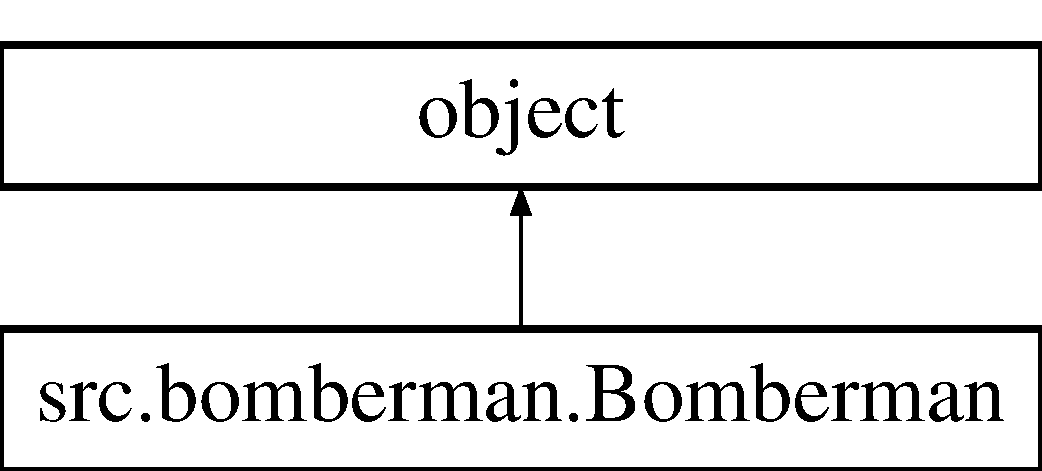
\includegraphics[height=2.000000cm]{classsrc_1_1bomberman_1_1_bomberman}
\end{center}
\end{figure}
\subsection*{Public Member Functions}
\begin{DoxyCompactItemize}
\item 
\hypertarget{classsrc_1_1bomberman_1_1_bomberman_ad9cdb2bcd44e1aaec299743531de5473}{}def \hyperlink{classsrc_1_1bomberman_1_1_bomberman_ad9cdb2bcd44e1aaec299743531de5473}{\+\_\+\+\_\+init\+\_\+\+\_\+} (self)\label{classsrc_1_1bomberman_1_1_bomberman_ad9cdb2bcd44e1aaec299743531de5473}

\begin{DoxyCompactList}\small\item\em Constructor of a bomberman unit with attributes. \end{DoxyCompactList}\item 
\hypertarget{classsrc_1_1bomberman_1_1_bomberman_a7d6de2893ff7ce0bed4cd72f15e9eb20}{}def \hyperlink{classsrc_1_1bomberman_1_1_bomberman_a7d6de2893ff7ce0bed4cd72f15e9eb20}{reset} (self)\label{classsrc_1_1bomberman_1_1_bomberman_a7d6de2893ff7ce0bed4cd72f15e9eb20}

\begin{DoxyCompactList}\small\item\em This method resets \hyperlink{classsrc_1_1bomberman_1_1_bomberman}{Bomberman}\textquotesingle{}s attribute at the start of a new level or a new game. \end{DoxyCompactList}\item 
\hypertarget{classsrc_1_1bomberman_1_1_bomberman_ae596075451ff8d73d59ff2cf9e4f7848}{}def \hyperlink{classsrc_1_1bomberman_1_1_bomberman_ae596075451ff8d73d59ff2cf9e4f7848}{death} (self)\label{classsrc_1_1bomberman_1_1_bomberman_ae596075451ff8d73d59ff2cf9e4f7848}

\begin{DoxyCompactList}\small\item\em This method resets \hyperlink{classsrc_1_1bomberman_1_1_bomberman}{Bomberman}\textquotesingle{}s attributes as well a its powerup and reduce its lives by 1. \end{DoxyCompactList}\end{DoxyCompactItemize}
\subsection*{Public Attributes}
\begin{DoxyCompactItemize}
\item 
\hypertarget{classsrc_1_1bomberman_1_1_bomberman_ade28c12524be42994d93b74bddc92647}{}\hyperlink{classsrc_1_1bomberman_1_1_bomberman_ade28c12524be42994d93b74bddc92647}{cur\+X}\label{classsrc_1_1bomberman_1_1_bomberman_ade28c12524be42994d93b74bddc92647}

\begin{DoxyCompactList}\small\item\em \hyperlink{classsrc_1_1bomberman_1_1_bomberman}{Bomberman}\textquotesingle{}s current X position. \end{DoxyCompactList}\item 
\hypertarget{classsrc_1_1bomberman_1_1_bomberman_ab163853c4ad07078948a14fc3b6ad1e7}{}\hyperlink{classsrc_1_1bomberman_1_1_bomberman_ab163853c4ad07078948a14fc3b6ad1e7}{cur\+Y}\label{classsrc_1_1bomberman_1_1_bomberman_ab163853c4ad07078948a14fc3b6ad1e7}

\begin{DoxyCompactList}\small\item\em \hyperlink{classsrc_1_1bomberman_1_1_bomberman}{Bomberman}\textquotesingle{}s current Y position. \end{DoxyCompactList}\item 
\hypertarget{classsrc_1_1bomberman_1_1_bomberman_a139e60f5380a184bd42d356afab660ef}{}\hyperlink{classsrc_1_1bomberman_1_1_bomberman_a139e60f5380a184bd42d356afab660ef}{lives}\label{classsrc_1_1bomberman_1_1_bomberman_a139e60f5380a184bd42d356afab660ef}

\begin{DoxyCompactList}\small\item\em \hyperlink{classsrc_1_1bomberman_1_1_bomberman}{Bomberman}\textquotesingle{}s current remaining lives. \end{DoxyCompactList}\item 
\hypertarget{classsrc_1_1bomberman_1_1_bomberman_a6ac3e76b884ce72178bd068a4c40c05b}{}\hyperlink{classsrc_1_1bomberman_1_1_bomberman_a6ac3e76b884ce72178bd068a4c40c05b}{speed}\label{classsrc_1_1bomberman_1_1_bomberman_a6ac3e76b884ce72178bd068a4c40c05b}

\begin{DoxyCompactList}\small\item\em \hyperlink{classsrc_1_1bomberman_1_1_bomberman}{Bomberman}\textquotesingle{}s current speed. \end{DoxyCompactList}\item 
\hypertarget{classsrc_1_1bomberman_1_1_bomberman_a71c03f3d45e6d025a1dc65d1933abb0a}{}\hyperlink{classsrc_1_1bomberman_1_1_bomberman_a71c03f3d45e6d025a1dc65d1933abb0a}{can\+Move}\label{classsrc_1_1bomberman_1_1_bomberman_a71c03f3d45e6d025a1dc65d1933abb0a}

\begin{DoxyCompactList}\small\item\em Boolean whether bomberman can move or not. \end{DoxyCompactList}\item 
\hypertarget{classsrc_1_1bomberman_1_1_bomberman_a2cb3572c62ccccb8eb2383145d0d4f2e}{}\hyperlink{classsrc_1_1bomberman_1_1_bomberman_a2cb3572c62ccccb8eb2383145d0d4f2e}{num\+Bombs}\label{classsrc_1_1bomberman_1_1_bomberman_a2cb3572c62ccccb8eb2383145d0d4f2e}

\begin{DoxyCompactList}\small\item\em Integer states maximum number of bombs bomberman can lay. \end{DoxyCompactList}\item 
\hypertarget{classsrc_1_1bomberman_1_1_bomberman_a60e8708ab7b666aa01aeb3cf0660db92}{}\hyperlink{classsrc_1_1bomberman_1_1_bomberman_a60e8708ab7b666aa01aeb3cf0660db92}{range\+Of\+Bombs}\label{classsrc_1_1bomberman_1_1_bomberman_a60e8708ab7b666aa01aeb3cf0660db92}

\begin{DoxyCompactList}\small\item\em Integer powerup the range in terms of tiles, the bomb can reach. \end{DoxyCompactList}\item 
\hypertarget{classsrc_1_1bomberman_1_1_bomberman_a8f1c6898c8d82b94228c5d4361c389a4}{}\hyperlink{classsrc_1_1bomberman_1_1_bomberman_a8f1c6898c8d82b94228c5d4361c389a4}{wall\+Pass}\label{classsrc_1_1bomberman_1_1_bomberman_a8f1c6898c8d82b94228c5d4361c389a4}

\begin{DoxyCompactList}\small\item\em Boolean powerup True if bomberman can pass through bricks. \end{DoxyCompactList}\item 
\hypertarget{classsrc_1_1bomberman_1_1_bomberman_af3633e53e0443adbc59816892d516065}{}\hyperlink{classsrc_1_1bomberman_1_1_bomberman_af3633e53e0443adbc59816892d516065}{has\+Detonator}\label{classsrc_1_1bomberman_1_1_bomberman_af3633e53e0443adbc59816892d516065}

\begin{DoxyCompactList}\small\item\em Boolean powerup True if bomberman has a detonator powerup. \end{DoxyCompactList}\item 
\hypertarget{classsrc_1_1bomberman_1_1_bomberman_aca70e55b92691117f315e82d444188d4}{}\hyperlink{classsrc_1_1bomberman_1_1_bomberman_aca70e55b92691117f315e82d444188d4}{bomb\+Pass}\label{classsrc_1_1bomberman_1_1_bomberman_aca70e55b92691117f315e82d444188d4}

\begin{DoxyCompactList}\small\item\em Boolean powerup True if bomberman can pass through bombs. \end{DoxyCompactList}\item 
\hypertarget{classsrc_1_1bomberman_1_1_bomberman_a04139259920ddb2447a762bcbc8a53c4}{}\hyperlink{classsrc_1_1bomberman_1_1_bomberman_a04139259920ddb2447a762bcbc8a53c4}{flame\+Pass}\label{classsrc_1_1bomberman_1_1_bomberman_a04139259920ddb2447a762bcbc8a53c4}

\begin{DoxyCompactList}\small\item\em Boolean powerup True if bomberman does not die when touching flames. \end{DoxyCompactList}\item 
\hypertarget{classsrc_1_1bomberman_1_1_bomberman_a6a139150d8425b6bf1a8431a991fc0f1}{}\hyperlink{classsrc_1_1bomberman_1_1_bomberman_a6a139150d8425b6bf1a8431a991fc0f1}{invincible}\label{classsrc_1_1bomberman_1_1_bomberman_a6a139150d8425b6bf1a8431a991fc0f1}

\begin{DoxyCompactList}\small\item\em Boolean powerup True if bomberman cannot die. \end{DoxyCompactList}\end{DoxyCompactItemize}


\subsection{Detailed Description}
This class \hyperlink{classsrc_1_1bomberman_1_1_bomberman}{Bomberman} contains all the attributes describing the current state of bomberman. 

The documentation for this class was generated from the following file\+:\begin{DoxyCompactItemize}
\item 
src/bomberman.\+py\end{DoxyCompactItemize}

\hypertarget{classsrc_1_1database_1_1_database}{}\section{src.\+database.\+Database Class Reference}
\label{classsrc_1_1database_1_1_database}\index{src.\+database.\+Database@{src.\+database.\+Database}}


Class that handles the interface with database.  


\subsection*{Public Member Functions}
\begin{DoxyCompactItemize}
\item 
def \hyperlink{classsrc_1_1database_1_1_database_aab829b3386356e12ed7276c63e168269}{\+\_\+\+\_\+init\+\_\+\+\_\+}
\begin{DoxyCompactList}\small\item\em Constructor that connects to a sqlite database, and gets the \textquotesingle{}user\textquotesingle{} table from it. \end{DoxyCompactList}\item 
def \hyperlink{classsrc_1_1database_1_1_database_a9f2df42cc938c2eb8186104b2831afaa}{create\+User} (self, name, username, password)
\begin{DoxyCompactList}\small\item\em Create a new user in the database. \end{DoxyCompactList}\item 
def \hyperlink{classsrc_1_1database_1_1_database_a374cf7a2b0dc2d1764fea49ef248544c}{update\+User\+Account} (self, old\+Username, new\+Username, new\+Realname, new\+Password)
\begin{DoxyCompactList}\small\item\em Update user account information with new username, realname, and password. \end{DoxyCompactList}\item 
def \hyperlink{classsrc_1_1database_1_1_database_ab38097adf50de7cdc08953819dc59d91}{delete\+Account} (self, username)
\begin{DoxyCompactList}\small\item\em Delete the account from the database. \end{DoxyCompactList}\item 
def \hyperlink{classsrc_1_1database_1_1_database_a801015f444b4267274d219381e134575}{check\+User} (self, username, password)
\begin{DoxyCompactList}\small\item\em Check whether the provided credentials correspond to a valid user account in the database. \end{DoxyCompactList}\item 
def \hyperlink{classsrc_1_1database_1_1_database_a12d75fd9334f108d345cdbd3ee8816a9}{has\+User} (self, username)
\begin{DoxyCompactList}\small\item\em Check whether the provided user name exists in the database. \end{DoxyCompactList}\item 
def \hyperlink{classsrc_1_1database_1_1_database_ad5f2e607e41b9b4d1e956d1a9a229afa}{is\+Valid\+Username} (self, username)
\begin{DoxyCompactList}\small\item\em Check whether the username is at least 6 character long. \end{DoxyCompactList}\item 
def \hyperlink{classsrc_1_1database_1_1_database_ae1b03c0a444fc7600f6d6333b0270437}{is\+Valid\+Password} (self, password)
\begin{DoxyCompactList}\small\item\em Check whether a password is valid. \end{DoxyCompactList}\item 
\hypertarget{classsrc_1_1database_1_1_database_a5bcb118c8b6079d851a6adb429eae756}{}def {\bfseries create\+User\+Accounts\+For\+Demo} (self)\label{classsrc_1_1database_1_1_database_a5bcb118c8b6079d851a6adb429eae756}

\item 
def \hyperlink{classsrc_1_1database_1_1_database_a18158514f653442eb3ff7bb61b5f5213}{get\+User\+Account} (self, username)
\begin{DoxyCompactList}\small\item\em Get the User\+Account object as a dictionary from the database. \end{DoxyCompactList}\item 
def \hyperlink{classsrc_1_1database_1_1_database_a1e26b95f30986a81d197e118420d0865}{get\+Top\+Ten\+Users} (self)
\begin{DoxyCompactList}\small\item\em Get top players sorted by cumulative score. \end{DoxyCompactList}\item 
def \hyperlink{classsrc_1_1database_1_1_database_a20befecd8b13cac9a87e59b759a5406a}{get\+Highest\+Unlocked\+Level} (self, username)
\begin{DoxyCompactList}\small\item\em Get highest unlocked level by the user. \end{DoxyCompactList}\item 
def \hyperlink{classsrc_1_1database_1_1_database_a0910f9e8e11bf94dcf9a24489e6f4dde}{save\+Game} (self, username, gamename, board)
\begin{DoxyCompactList}\small\item\em Save current game state into a file. \end{DoxyCompactList}\item 
def \hyperlink{classsrc_1_1database_1_1_database_a8f48d5d1c090840389e7cbc556d635b5}{load\+List\+Saved\+Games} (self, username)
\begin{DoxyCompactList}\small\item\em Load the list of previously saved games for an user. \end{DoxyCompactList}\item 
def \hyperlink{classsrc_1_1database_1_1_database_abc4a7e44498f2e3ede0c52a43725526d}{load\+Game} (self, username, gamename)
\begin{DoxyCompactList}\small\item\em Load a specific game for an user. \end{DoxyCompactList}\item 
def \hyperlink{classsrc_1_1database_1_1_database_aea1e0de87f1e08cf83d31a2179cf0c12}{update\+User\+Score} (self, username, score\+To\+Add)
\begin{DoxyCompactList}\small\item\em Update the user\textquotesingle{}s cumulative score in the database. \end{DoxyCompactList}\item 
def \hyperlink{classsrc_1_1database_1_1_database_adf6d7572d1782bedb86e6880c24e8e9e}{increment\+Num\+Of\+Games\+Played} (self, username)
\begin{DoxyCompactList}\small\item\em Increment the total number of games played for the user. \end{DoxyCompactList}\end{DoxyCompactItemize}
\subsection*{Public Attributes}
\begin{DoxyCompactItemize}
\item 
\hypertarget{classsrc_1_1database_1_1_database_a3b1c6af40f8d2c934bf2d63d71e657e5}{}{\bfseries db}\label{classsrc_1_1database_1_1_database_a3b1c6af40f8d2c934bf2d63d71e657e5}

\item 
\hypertarget{classsrc_1_1database_1_1_database_a7b7d83448ad1895241783bf04a5a1b6c}{}{\bfseries user\+Table}\label{classsrc_1_1database_1_1_database_a7b7d83448ad1895241783bf04a5a1b6c}

\item 
\hypertarget{classsrc_1_1database_1_1_database_a50ceb943a93153787b40bb9c037049aa}{}{\bfseries game}\label{classsrc_1_1database_1_1_database_a50ceb943a93153787b40bb9c037049aa}

\end{DoxyCompactItemize}


\subsection{Detailed Description}
Class that handles the interface with database. 

An instance of this class connects to a local sqlite database with a single table. The table stores each attribute of \hyperlink{classsrc_1_1models_1_1_user_account}{models.\+User\+Account} as a column, with the username being the primary key. 

\subsection{Constructor \& Destructor Documentation}
\hypertarget{classsrc_1_1database_1_1_database_aab829b3386356e12ed7276c63e168269}{}\index{src\+::database\+::\+Database@{src\+::database\+::\+Database}!\+\_\+\+\_\+init\+\_\+\+\_\+@{\+\_\+\+\_\+init\+\_\+\+\_\+}}
\index{\+\_\+\+\_\+init\+\_\+\+\_\+@{\+\_\+\+\_\+init\+\_\+\+\_\+}!src\+::database\+::\+Database@{src\+::database\+::\+Database}}
\subsubsection[{\+\_\+\+\_\+init\+\_\+\+\_\+}]{\setlength{\rightskip}{0pt plus 5cm}def src.\+database.\+Database.\+\_\+\+\_\+init\+\_\+\+\_\+ (
\begin{DoxyParamCaption}
\item[{}]{self, }
\item[{}]{test = {\ttfamily False}}
\end{DoxyParamCaption}
)}\label{classsrc_1_1database_1_1_database_aab829b3386356e12ed7276c63e168269}


Constructor that connects to a sqlite database, and gets the \textquotesingle{}user\textquotesingle{} table from it. 

It creates the database and the table if it cannot find them. 
\begin{DoxyParams}{Parameters}
{\em test} & By default False. If set to True, the database will be in memory instead of on the file system. Used in unit tests. \\
\hline
\end{DoxyParams}


\subsection{Member Function Documentation}
\hypertarget{classsrc_1_1database_1_1_database_a801015f444b4267274d219381e134575}{}\index{src\+::database\+::\+Database@{src\+::database\+::\+Database}!check\+User@{check\+User}}
\index{check\+User@{check\+User}!src\+::database\+::\+Database@{src\+::database\+::\+Database}}
\subsubsection[{check\+User}]{\setlength{\rightskip}{0pt plus 5cm}def src.\+database.\+Database.\+check\+User (
\begin{DoxyParamCaption}
\item[{}]{self, }
\item[{}]{username, }
\item[{}]{password}
\end{DoxyParamCaption}
)}\label{classsrc_1_1database_1_1_database_a801015f444b4267274d219381e134575}


Check whether the provided credentials correspond to a valid user account in the database. 


\begin{DoxyParams}{Parameters}
{\em username} & the username to be checked \\
\hline
{\em password} & the password to be checked \\
\hline
\end{DoxyParams}
\begin{DoxyReturn}{Returns}
True if the username exists, False otherwise 
\end{DoxyReturn}
\hypertarget{classsrc_1_1database_1_1_database_a9f2df42cc938c2eb8186104b2831afaa}{}\index{src\+::database\+::\+Database@{src\+::database\+::\+Database}!create\+User@{create\+User}}
\index{create\+User@{create\+User}!src\+::database\+::\+Database@{src\+::database\+::\+Database}}
\subsubsection[{create\+User}]{\setlength{\rightskip}{0pt plus 5cm}def src.\+database.\+Database.\+create\+User (
\begin{DoxyParamCaption}
\item[{}]{self, }
\item[{}]{name, }
\item[{}]{username, }
\item[{}]{password}
\end{DoxyParamCaption}
)}\label{classsrc_1_1database_1_1_database_a9f2df42cc938c2eb8186104b2831afaa}


Create a new user in the database. 


\begin{DoxyParams}{Parameters}
{\em name} & the real name \\
\hline
{\em username} & the username \\
\hline
{\em password} & the password \\
\hline
\end{DoxyParams}
\begin{DoxyReturn}{Returns}
True if user account properly created, False if user already exists 
\end{DoxyReturn}
\hypertarget{classsrc_1_1database_1_1_database_ab38097adf50de7cdc08953819dc59d91}{}\index{src\+::database\+::\+Database@{src\+::database\+::\+Database}!delete\+Account@{delete\+Account}}
\index{delete\+Account@{delete\+Account}!src\+::database\+::\+Database@{src\+::database\+::\+Database}}
\subsubsection[{delete\+Account}]{\setlength{\rightskip}{0pt plus 5cm}def src.\+database.\+Database.\+delete\+Account (
\begin{DoxyParamCaption}
\item[{}]{self, }
\item[{}]{username}
\end{DoxyParamCaption}
)}\label{classsrc_1_1database_1_1_database_ab38097adf50de7cdc08953819dc59d91}


Delete the account from the database. 


\begin{DoxyParams}{Parameters}
{\em username} & the user we want to delete \\
\hline
\end{DoxyParams}
\hypertarget{classsrc_1_1database_1_1_database_a20befecd8b13cac9a87e59b759a5406a}{}\index{src\+::database\+::\+Database@{src\+::database\+::\+Database}!get\+Highest\+Unlocked\+Level@{get\+Highest\+Unlocked\+Level}}
\index{get\+Highest\+Unlocked\+Level@{get\+Highest\+Unlocked\+Level}!src\+::database\+::\+Database@{src\+::database\+::\+Database}}
\subsubsection[{get\+Highest\+Unlocked\+Level}]{\setlength{\rightskip}{0pt plus 5cm}def src.\+database.\+Database.\+get\+Highest\+Unlocked\+Level (
\begin{DoxyParamCaption}
\item[{}]{self, }
\item[{}]{username}
\end{DoxyParamCaption}
)}\label{classsrc_1_1database_1_1_database_a20befecd8b13cac9a87e59b759a5406a}


Get highest unlocked level by the user. 


\begin{DoxyParams}{Parameters}
{\em username} & the user for whom we want to get the highest unlocked level \\
\hline
\end{DoxyParams}
\begin{DoxyReturn}{Returns}
the highest unlocked level of that user 
\end{DoxyReturn}
\hypertarget{classsrc_1_1database_1_1_database_a1e26b95f30986a81d197e118420d0865}{}\index{src\+::database\+::\+Database@{src\+::database\+::\+Database}!get\+Top\+Ten\+Users@{get\+Top\+Ten\+Users}}
\index{get\+Top\+Ten\+Users@{get\+Top\+Ten\+Users}!src\+::database\+::\+Database@{src\+::database\+::\+Database}}
\subsubsection[{get\+Top\+Ten\+Users}]{\setlength{\rightskip}{0pt plus 5cm}def src.\+database.\+Database.\+get\+Top\+Ten\+Users (
\begin{DoxyParamCaption}
\item[{}]{self}
\end{DoxyParamCaption}
)}\label{classsrc_1_1database_1_1_database_a1e26b95f30986a81d197e118420d0865}


Get top players sorted by cumulative score. 

Same score is counted as two. Users with the same score are sorted alphabetically (by username). \begin{DoxyReturn}{Returns}
a iterable list of User\+Account objects as dictionaries 
\end{DoxyReturn}
\hypertarget{classsrc_1_1database_1_1_database_a18158514f653442eb3ff7bb61b5f5213}{}\index{src\+::database\+::\+Database@{src\+::database\+::\+Database}!get\+User\+Account@{get\+User\+Account}}
\index{get\+User\+Account@{get\+User\+Account}!src\+::database\+::\+Database@{src\+::database\+::\+Database}}
\subsubsection[{get\+User\+Account}]{\setlength{\rightskip}{0pt plus 5cm}def src.\+database.\+Database.\+get\+User\+Account (
\begin{DoxyParamCaption}
\item[{}]{self, }
\item[{}]{username}
\end{DoxyParamCaption}
)}\label{classsrc_1_1database_1_1_database_a18158514f653442eb3ff7bb61b5f5213}


Get the User\+Account object as a dictionary from the database. 


\begin{DoxyParams}{Parameters}
{\em username} & the username used as a key to retrieve the User\+Account \\
\hline
\end{DoxyParams}
\begin{DoxyReturn}{Returns}
the User\+Account object as a dictionary 
\end{DoxyReturn}
\hypertarget{classsrc_1_1database_1_1_database_a12d75fd9334f108d345cdbd3ee8816a9}{}\index{src\+::database\+::\+Database@{src\+::database\+::\+Database}!has\+User@{has\+User}}
\index{has\+User@{has\+User}!src\+::database\+::\+Database@{src\+::database\+::\+Database}}
\subsubsection[{has\+User}]{\setlength{\rightskip}{0pt plus 5cm}def src.\+database.\+Database.\+has\+User (
\begin{DoxyParamCaption}
\item[{}]{self, }
\item[{}]{username}
\end{DoxyParamCaption}
)}\label{classsrc_1_1database_1_1_database_a12d75fd9334f108d345cdbd3ee8816a9}


Check whether the provided user name exists in the database. 


\begin{DoxyParams}{Parameters}
{\em username} & the username to be checked \\
\hline
\end{DoxyParams}
\hypertarget{classsrc_1_1database_1_1_database_adf6d7572d1782bedb86e6880c24e8e9e}{}\index{src\+::database\+::\+Database@{src\+::database\+::\+Database}!increment\+Num\+Of\+Games\+Played@{increment\+Num\+Of\+Games\+Played}}
\index{increment\+Num\+Of\+Games\+Played@{increment\+Num\+Of\+Games\+Played}!src\+::database\+::\+Database@{src\+::database\+::\+Database}}
\subsubsection[{increment\+Num\+Of\+Games\+Played}]{\setlength{\rightskip}{0pt plus 5cm}def src.\+database.\+Database.\+increment\+Num\+Of\+Games\+Played (
\begin{DoxyParamCaption}
\item[{}]{self, }
\item[{}]{username}
\end{DoxyParamCaption}
)}\label{classsrc_1_1database_1_1_database_adf6d7572d1782bedb86e6880c24e8e9e}


Increment the total number of games played for the user. 


\begin{DoxyParams}{Parameters}
{\em username} & the user for whom we want to increment the number of games played \\
\hline
\end{DoxyParams}
\hypertarget{classsrc_1_1database_1_1_database_ae1b03c0a444fc7600f6d6333b0270437}{}\index{src\+::database\+::\+Database@{src\+::database\+::\+Database}!is\+Valid\+Password@{is\+Valid\+Password}}
\index{is\+Valid\+Password@{is\+Valid\+Password}!src\+::database\+::\+Database@{src\+::database\+::\+Database}}
\subsubsection[{is\+Valid\+Password}]{\setlength{\rightskip}{0pt plus 5cm}def src.\+database.\+Database.\+is\+Valid\+Password (
\begin{DoxyParamCaption}
\item[{}]{self, }
\item[{}]{password}
\end{DoxyParamCaption}
)}\label{classsrc_1_1database_1_1_database_ae1b03c0a444fc7600f6d6333b0270437}


Check whether a password is valid. 

A valid password must be at least 8 characters long. In addition, it must necessarily include a minimum of 1 Upper case letter, 1 Lower case letter, 1 digits and 1 special character. 
\begin{DoxyParams}{Parameters}
{\em password} & the password to be checked \\
\hline
\end{DoxyParams}
\begin{DoxyReturn}{Returns}
True if the password is valid, False otherwise 
\end{DoxyReturn}
\hypertarget{classsrc_1_1database_1_1_database_ad5f2e607e41b9b4d1e956d1a9a229afa}{}\index{src\+::database\+::\+Database@{src\+::database\+::\+Database}!is\+Valid\+Username@{is\+Valid\+Username}}
\index{is\+Valid\+Username@{is\+Valid\+Username}!src\+::database\+::\+Database@{src\+::database\+::\+Database}}
\subsubsection[{is\+Valid\+Username}]{\setlength{\rightskip}{0pt plus 5cm}def src.\+database.\+Database.\+is\+Valid\+Username (
\begin{DoxyParamCaption}
\item[{}]{self, }
\item[{}]{username}
\end{DoxyParamCaption}
)}\label{classsrc_1_1database_1_1_database_ad5f2e607e41b9b4d1e956d1a9a229afa}


Check whether the username is at least 6 character long. 


\begin{DoxyParams}{Parameters}
{\em username} & the username to be checked \\
\hline
\end{DoxyParams}
\begin{DoxyReturn}{Returns}
True if the username is valid, False otherwise 
\end{DoxyReturn}
\hypertarget{classsrc_1_1database_1_1_database_abc4a7e44498f2e3ede0c52a43725526d}{}\index{src\+::database\+::\+Database@{src\+::database\+::\+Database}!load\+Game@{load\+Game}}
\index{load\+Game@{load\+Game}!src\+::database\+::\+Database@{src\+::database\+::\+Database}}
\subsubsection[{load\+Game}]{\setlength{\rightskip}{0pt plus 5cm}def src.\+database.\+Database.\+load\+Game (
\begin{DoxyParamCaption}
\item[{}]{self, }
\item[{}]{username, }
\item[{}]{gamename}
\end{DoxyParamCaption}
)}\label{classsrc_1_1database_1_1_database_abc4a7e44498f2e3ede0c52a43725526d}


Load a specific game for an user. 


\begin{DoxyParams}{Parameters}
{\em username} & the user for whom we want to load the game \\
\hline
{\em gamename} & the name of the game we want to load \\
\hline
\end{DoxyParams}
\hypertarget{classsrc_1_1database_1_1_database_a8f48d5d1c090840389e7cbc556d635b5}{}\index{src\+::database\+::\+Database@{src\+::database\+::\+Database}!load\+List\+Saved\+Games@{load\+List\+Saved\+Games}}
\index{load\+List\+Saved\+Games@{load\+List\+Saved\+Games}!src\+::database\+::\+Database@{src\+::database\+::\+Database}}
\subsubsection[{load\+List\+Saved\+Games}]{\setlength{\rightskip}{0pt plus 5cm}def src.\+database.\+Database.\+load\+List\+Saved\+Games (
\begin{DoxyParamCaption}
\item[{}]{self, }
\item[{}]{username}
\end{DoxyParamCaption}
)}\label{classsrc_1_1database_1_1_database_a8f48d5d1c090840389e7cbc556d635b5}


Load the list of previously saved games for an user. 


\begin{DoxyParams}{Parameters}
{\em username} & the user for whom we want to load the list of saved game \\
\hline
\end{DoxyParams}
\hypertarget{classsrc_1_1database_1_1_database_a0910f9e8e11bf94dcf9a24489e6f4dde}{}\index{src\+::database\+::\+Database@{src\+::database\+::\+Database}!save\+Game@{save\+Game}}
\index{save\+Game@{save\+Game}!src\+::database\+::\+Database@{src\+::database\+::\+Database}}
\subsubsection[{save\+Game}]{\setlength{\rightskip}{0pt plus 5cm}def src.\+database.\+Database.\+save\+Game (
\begin{DoxyParamCaption}
\item[{}]{self, }
\item[{}]{username, }
\item[{}]{gamename, }
\item[{}]{board}
\end{DoxyParamCaption}
)}\label{classsrc_1_1database_1_1_database_a0910f9e8e11bf94dcf9a24489e6f4dde}


Save current game state into a file. 


\begin{DoxyParams}{Parameters}
{\em username} & the user for whom we want to save the game \\
\hline
{\em gamename} & the name of the game we want to save \\
\hline
{\em board} & the current board containing all game state that needs to be saved \\
\hline
\end{DoxyParams}
\hypertarget{classsrc_1_1database_1_1_database_a374cf7a2b0dc2d1764fea49ef248544c}{}\index{src\+::database\+::\+Database@{src\+::database\+::\+Database}!update\+User\+Account@{update\+User\+Account}}
\index{update\+User\+Account@{update\+User\+Account}!src\+::database\+::\+Database@{src\+::database\+::\+Database}}
\subsubsection[{update\+User\+Account}]{\setlength{\rightskip}{0pt plus 5cm}def src.\+database.\+Database.\+update\+User\+Account (
\begin{DoxyParamCaption}
\item[{}]{self, }
\item[{}]{old\+Username, }
\item[{}]{new\+Username, }
\item[{}]{new\+Realname, }
\item[{}]{new\+Password}
\end{DoxyParamCaption}
)}\label{classsrc_1_1database_1_1_database_a374cf7a2b0dc2d1764fea49ef248544c}


Update user account information with new username, realname, and password. 


\begin{DoxyParams}{Parameters}
{\em old\+Username} & the old user name with which we retrieve the account \\
\hline
{\em new\+Username} & the new user name we want to set \\
\hline
{\em new\+Realname} & the new real name we want to set \\
\hline
{\em new\+Password} & the new password we want to set \\
\hline
\end{DoxyParams}
\hypertarget{classsrc_1_1database_1_1_database_aea1e0de87f1e08cf83d31a2179cf0c12}{}\index{src\+::database\+::\+Database@{src\+::database\+::\+Database}!update\+User\+Score@{update\+User\+Score}}
\index{update\+User\+Score@{update\+User\+Score}!src\+::database\+::\+Database@{src\+::database\+::\+Database}}
\subsubsection[{update\+User\+Score}]{\setlength{\rightskip}{0pt plus 5cm}def src.\+database.\+Database.\+update\+User\+Score (
\begin{DoxyParamCaption}
\item[{}]{self, }
\item[{}]{username, }
\item[{}]{score\+To\+Add}
\end{DoxyParamCaption}
)}\label{classsrc_1_1database_1_1_database_aea1e0de87f1e08cf83d31a2179cf0c12}


Update the user\textquotesingle{}s cumulative score in the database. 


\begin{DoxyParams}{Parameters}
{\em username} & the user for whom we want to update the score \\
\hline
{\em score\+To\+Add} & the score we want to add to the existing cumulative score in the database \\
\hline
\end{DoxyParams}


The documentation for this class was generated from the following file\+:\begin{DoxyCompactItemize}
\item 
src/database.\+py\end{DoxyCompactItemize}

\hypertarget{classsrc_1_1enemy_1_1_enemy}{}\section{src.\+enemy.\+Enemy Class Reference}
\label{classsrc_1_1enemy_1_1_enemy}\index{src.\+enemy.\+Enemy@{src.\+enemy.\+Enemy}}
Inheritance diagram for src.\+enemy.\+Enemy\+:\begin{figure}[H]
\begin{center}
\leavevmode
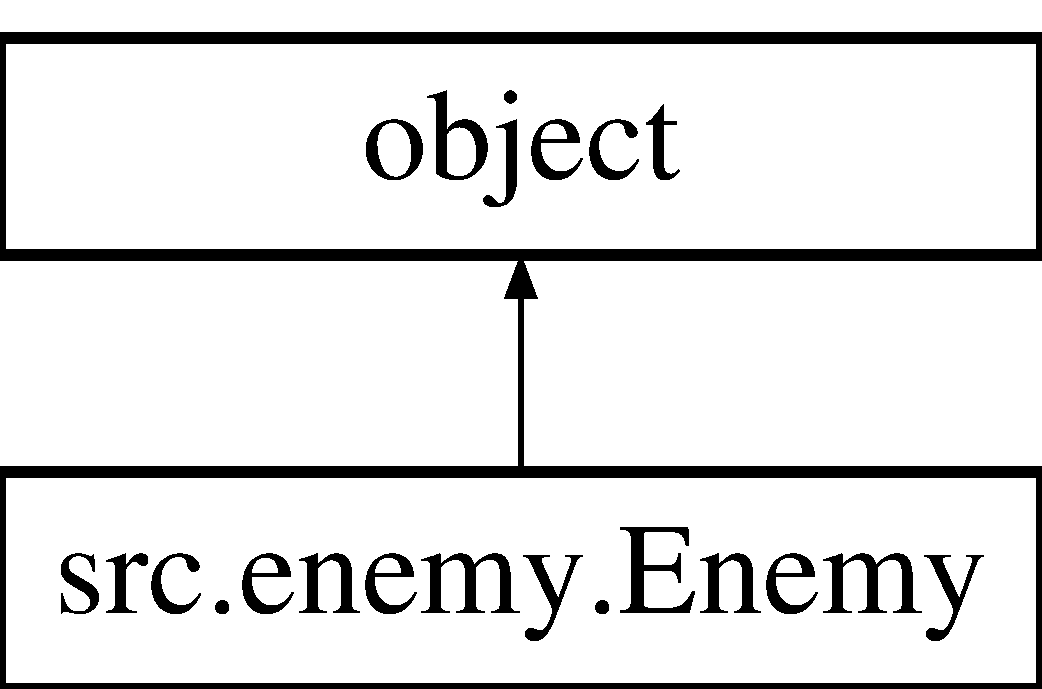
\includegraphics[height=2.000000cm]{classsrc_1_1enemy_1_1_enemy}
\end{center}
\end{figure}
\subsection*{Public Member Functions}
\begin{DoxyCompactItemize}
\item 
\hypertarget{classsrc_1_1enemy_1_1_enemy_a6ec62571df1087a1a7683d62a4434081}{}def {\bfseries \+\_\+\+\_\+init\+\_\+\+\_\+} (self, points, speed, intelligence, wallpass, direction, can\+Move)\label{classsrc_1_1enemy_1_1_enemy_a6ec62571df1087a1a7683d62a4434081}

\end{DoxyCompactItemize}
\subsection*{Static Public Member Functions}
\begin{DoxyCompactItemize}
\item 
\hypertarget{classsrc_1_1enemy_1_1_enemy_a4476f5bc0be70d26bebece6abcb7bdad}{}def {\bfseries get\+Enemy} (type)\label{classsrc_1_1enemy_1_1_enemy_a4476f5bc0be70d26bebece6abcb7bdad}

\item 
\hypertarget{classsrc_1_1enemy_1_1_enemy_a01da6a5d5f8eb5db75323749a80fc3a0}{}def {\bfseries get\+Enemy\+List\+And\+Power\+Up} (level)\label{classsrc_1_1enemy_1_1_enemy_a01da6a5d5f8eb5db75323749a80fc3a0}

\end{DoxyCompactItemize}
\subsection*{Public Attributes}
\begin{DoxyCompactItemize}
\item 
\hypertarget{classsrc_1_1enemy_1_1_enemy_ae9fc7353b9fbbad3c2d0330169a14fe5}{}{\bfseries points}\label{classsrc_1_1enemy_1_1_enemy_ae9fc7353b9fbbad3c2d0330169a14fe5}

\item 
\hypertarget{classsrc_1_1enemy_1_1_enemy_a24e64f3d82db0537f8438780bb1b082d}{}{\bfseries speed}\label{classsrc_1_1enemy_1_1_enemy_a24e64f3d82db0537f8438780bb1b082d}

\item 
\hypertarget{classsrc_1_1enemy_1_1_enemy_a11c139459feab2281e0804adc1e0276d}{}{\bfseries intelligence}\label{classsrc_1_1enemy_1_1_enemy_a11c139459feab2281e0804adc1e0276d}

\item 
\hypertarget{classsrc_1_1enemy_1_1_enemy_a3efd2aacdc7f1eca427075919649c09e}{}{\bfseries wallpass}\label{classsrc_1_1enemy_1_1_enemy_a3efd2aacdc7f1eca427075919649c09e}

\item 
\hypertarget{classsrc_1_1enemy_1_1_enemy_ad232e0c586291fffbc676d6b20658cd2}{}{\bfseries direction}\label{classsrc_1_1enemy_1_1_enemy_ad232e0c586291fffbc676d6b20658cd2}

\item 
\hypertarget{classsrc_1_1enemy_1_1_enemy_aca96a4793e02437f1f33a1c3cbefd133}{}{\bfseries can\+Move}\label{classsrc_1_1enemy_1_1_enemy_aca96a4793e02437f1f33a1c3cbefd133}

\end{DoxyCompactItemize}


The documentation for this class was generated from the following file\+:\begin{DoxyCompactItemize}
\item 
src/enemy.\+py\end{DoxyCompactItemize}

\hypertarget{classsrc_1_1game_1_1_game}{}\section{src.\+game.\+Game Class Reference}
\label{classsrc_1_1game_1_1_game}\index{src.\+game.\+Game@{src.\+game.\+Game}}


Main controller.  


Inheritance diagram for src.\+game.\+Game\+:\begin{figure}[H]
\begin{center}
\leavevmode
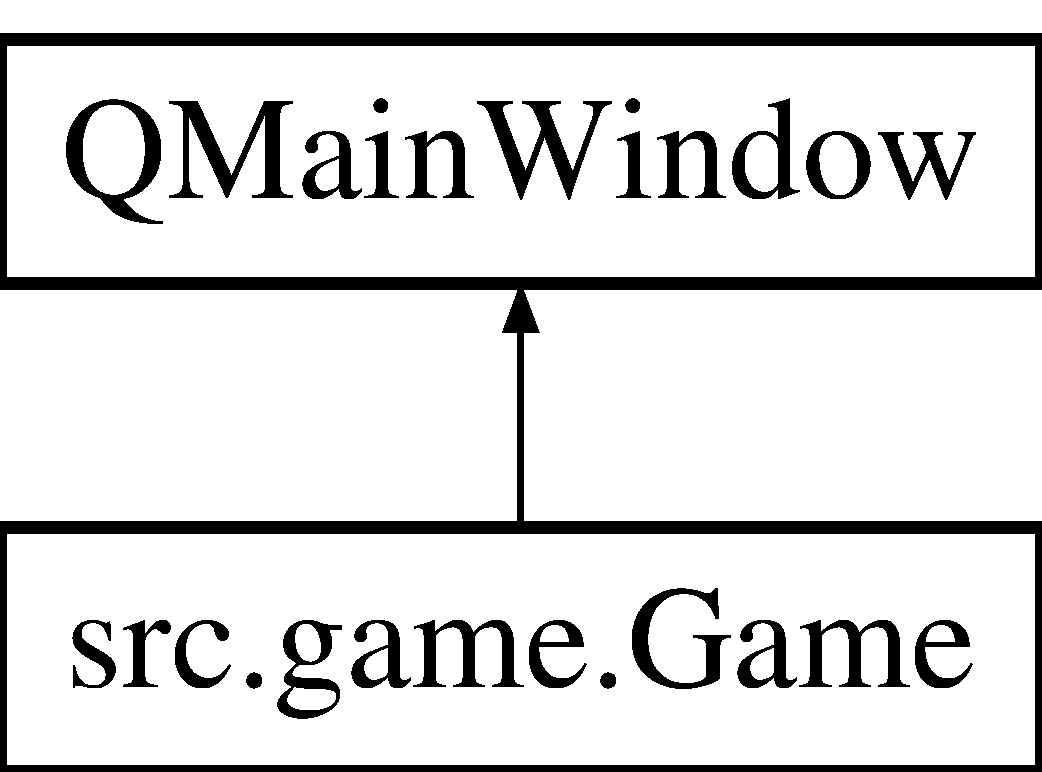
\includegraphics[height=2.000000cm]{classsrc_1_1game_1_1_game}
\end{center}
\end{figure}
\subsection*{Public Member Functions}
\begin{DoxyCompactItemize}
\item 
\hypertarget{classsrc_1_1game_1_1_game_a15684812af57df03feb870c9b4b380a2}{}def \hyperlink{classsrc_1_1game_1_1_game_a15684812af57df03feb870c9b4b380a2}{\+\_\+\+\_\+init\+\_\+\+\_\+} (self)\label{classsrc_1_1game_1_1_game_a15684812af57df03feb870c9b4b380a2}

\begin{DoxyCompactList}\small\item\em Constructor, initializes U\+I. \end{DoxyCompactList}\item 
\hypertarget{classsrc_1_1game_1_1_game_a89ba31b71efebcc9b2f43227d833e38f}{}def \hyperlink{classsrc_1_1game_1_1_game_a89ba31b71efebcc9b2f43227d833e38f}{init\+U\+I} (self)\label{classsrc_1_1game_1_1_game_a89ba31b71efebcc9b2f43227d833e38f}

\begin{DoxyCompactList}\small\item\em This method initializes the U\+I and center the window. \end{DoxyCompactList}\item 
\hypertarget{classsrc_1_1game_1_1_game_a7a14788a82ebc0d4b4b821ac1489a7a0}{}def \hyperlink{classsrc_1_1game_1_1_game_a7a14788a82ebc0d4b4b821ac1489a7a0}{show\+Login\+Menu} (self)\label{classsrc_1_1game_1_1_game_a7a14788a82ebc0d4b4b821ac1489a7a0}

\begin{DoxyCompactList}\small\item\em This method displays the login menu. \end{DoxyCompactList}\item 
\hypertarget{classsrc_1_1game_1_1_game_a218f9c8c6e86a19fa9d3155ce43068a0}{}def \hyperlink{classsrc_1_1game_1_1_game_a218f9c8c6e86a19fa9d3155ce43068a0}{show\+Main\+Menu} (self)\label{classsrc_1_1game_1_1_game_a218f9c8c6e86a19fa9d3155ce43068a0}

\begin{DoxyCompactList}\small\item\em This method displays the login menu after successful login. \end{DoxyCompactList}\item 
\hypertarget{classsrc_1_1game_1_1_game_afe69a6fa066d92365c226aff1c903e90}{}def \hyperlink{classsrc_1_1game_1_1_game_afe69a6fa066d92365c226aff1c903e90}{show\+Level\+Menu} (self)\label{classsrc_1_1game_1_1_game_afe69a6fa066d92365c226aff1c903e90}

\begin{DoxyCompactList}\small\item\em This method displays the level menu where player is asked to select level to play. \end{DoxyCompactList}\item 
def \hyperlink{classsrc_1_1game_1_1_game_a570dba568ad9dd3b9745e0f10a4b29a8}{show\+Board}
\begin{DoxyCompactList}\small\item\em This method displays the bomberman gameplay and initiliazes the game to the selected level. \end{DoxyCompactList}\item 
\hypertarget{classsrc_1_1game_1_1_game_a13a6d564b3397c8c520b0b23e99d0880}{}def \hyperlink{classsrc_1_1game_1_1_game_a13a6d564b3397c8c520b0b23e99d0880}{show\+Leaderboard} (self, previous\+Menu)\label{classsrc_1_1game_1_1_game_a13a6d564b3397c8c520b0b23e99d0880}

\begin{DoxyCompactList}\small\item\em This method isplays the leaderboard. \end{DoxyCompactList}\item 
\hypertarget{classsrc_1_1game_1_1_game_a0e17658d314189179aa5be0bfdc185da}{}def \hyperlink{classsrc_1_1game_1_1_game_a0e17658d314189179aa5be0bfdc185da}{show\+Pause\+Menu} (self)\label{classsrc_1_1game_1_1_game_a0e17658d314189179aa5be0bfdc185da}

\begin{DoxyCompactList}\small\item\em This method displays pause menu. \end{DoxyCompactList}\item 
\hypertarget{classsrc_1_1game_1_1_game_a02ee6b88570e0af0686050a2268f687b}{}def \hyperlink{classsrc_1_1game_1_1_game_a02ee6b88570e0af0686050a2268f687b}{show\+Save\+Menu} (self)\label{classsrc_1_1game_1_1_game_a02ee6b88570e0af0686050a2268f687b}

\begin{DoxyCompactList}\small\item\em This method displays the menu to save game instances. \end{DoxyCompactList}\item 
\hypertarget{classsrc_1_1game_1_1_game_a4c38f9b4c2f4e81a49e25632dccd8622}{}def \hyperlink{classsrc_1_1game_1_1_game_a4c38f9b4c2f4e81a49e25632dccd8622}{show\+Load\+Menu} (self, previous\+Menu)\label{classsrc_1_1game_1_1_game_a4c38f9b4c2f4e81a49e25632dccd8622}

\begin{DoxyCompactList}\small\item\em This method displays the menu to load saved game instances. \end{DoxyCompactList}\item 
\hypertarget{classsrc_1_1game_1_1_game_a42b40336207a65cb12910ae7d1a4175d}{}def \hyperlink{classsrc_1_1game_1_1_game_a42b40336207a65cb12910ae7d1a4175d}{show\+Account\+Settings\+Menu} (self)\label{classsrc_1_1game_1_1_game_a42b40336207a65cb12910ae7d1a4175d}

\begin{DoxyCompactList}\small\item\em This method displays the account settings menu. \end{DoxyCompactList}\item 
\hypertarget{classsrc_1_1game_1_1_game_a243a1df9b63a0f081b90fa29146a4af6}{}def \hyperlink{classsrc_1_1game_1_1_game_a243a1df9b63a0f081b90fa29146a4af6}{center} (self)\label{classsrc_1_1game_1_1_game_a243a1df9b63a0f081b90fa29146a4af6}

\begin{DoxyCompactList}\small\item\em This method centers the current window to the middle. \end{DoxyCompactList}\item 
\hypertarget{classsrc_1_1game_1_1_game_aa7856f8d00f279cc139d131cb2e8d8ea}{}def \hyperlink{classsrc_1_1game_1_1_game_aa7856f8d00f279cc139d131cb2e8d8ea}{quit} (self)\label{classsrc_1_1game_1_1_game_aa7856f8d00f279cc139d131cb2e8d8ea}

\begin{DoxyCompactList}\small\item\em This method exits the process. \end{DoxyCompactList}\item 
\hypertarget{classsrc_1_1game_1_1_game_a19d0646df1f0cb57f8262412487d5270}{}def \hyperlink{classsrc_1_1game_1_1_game_a19d0646df1f0cb57f8262412487d5270}{resume\+To\+Game} (self)\label{classsrc_1_1game_1_1_game_a19d0646df1f0cb57f8262412487d5270}

\begin{DoxyCompactList}\small\item\em This method resumes the game after a pause action. \end{DoxyCompactList}\item 
\hypertarget{classsrc_1_1game_1_1_game_add2df3ddda7fa333cadb6fcfa060eaef}{}def \hyperlink{classsrc_1_1game_1_1_game_add2df3ddda7fa333cadb6fcfa060eaef}{resume\+To\+Pause\+Menu} (self)\label{classsrc_1_1game_1_1_game_add2df3ddda7fa333cadb6fcfa060eaef}

\begin{DoxyCompactList}\small\item\em This method navigates back to pause menu. \end{DoxyCompactList}\item 
\hypertarget{classsrc_1_1game_1_1_game_a8e215b6533b7fa858334453633e12e6e}{}def \hyperlink{classsrc_1_1game_1_1_game_a8e215b6533b7fa858334453633e12e6e}{load\+Saved\+Game} (self, gamename)\label{classsrc_1_1game_1_1_game_a8e215b6533b7fa858334453633e12e6e}

\begin{DoxyCompactList}\small\item\em This method loads the current user\textquotesingle{}s saved game instance corresponding to the provided game name. \end{DoxyCompactList}\item 
\hypertarget{classsrc_1_1game_1_1_game_ae864ef349cf3b094874543fab2210a37}{}def \hyperlink{classsrc_1_1game_1_1_game_ae864ef349cf3b094874543fab2210a37}{game\+Over} (self)\label{classsrc_1_1game_1_1_game_ae864ef349cf3b094874543fab2210a37}

\begin{DoxyCompactList}\small\item\em This method emits a signal to acknowledge game over state. \end{DoxyCompactList}\item 
\hypertarget{classsrc_1_1game_1_1_game_a85c98d60278dc78a465e40b5e3c57579}{}def \hyperlink{classsrc_1_1game_1_1_game_a85c98d60278dc78a465e40b5e3c57579}{update\+Score\+In\+Db} (self, incremental\+Score)\label{classsrc_1_1game_1_1_game_a85c98d60278dc78a465e40b5e3c57579}

\begin{DoxyCompactList}\small\item\em This method updates the user\textquotesingle{}s current score to the database. \end{DoxyCompactList}\item 
\hypertarget{classsrc_1_1game_1_1_game_a45770f3f952d2738b599e04ade877296}{}def \hyperlink{classsrc_1_1game_1_1_game_a45770f3f952d2738b599e04ade877296}{update\+Games\+Played\+In\+Db} (self)\label{classsrc_1_1game_1_1_game_a45770f3f952d2738b599e04ade877296}

\begin{DoxyCompactList}\small\item\em This method updates the users\textquotesingle{} number of games played to the database. \end{DoxyCompactList}\end{DoxyCompactItemize}
\subsection*{Public Attributes}
\begin{DoxyCompactItemize}
\item 
\hypertarget{classsrc_1_1game_1_1_game_a92c4f3cb7732c69c98cfb2ed60787493}{}{\bfseries central\+Widget}\label{classsrc_1_1game_1_1_game_a92c4f3cb7732c69c98cfb2ed60787493}

\item 
\hypertarget{classsrc_1_1game_1_1_game_a99d603ef9c1161c44a4f5a56bb6dd9f2}{}{\bfseries login\+Widget}\label{classsrc_1_1game_1_1_game_a99d603ef9c1161c44a4f5a56bb6dd9f2}

\item 
\hypertarget{classsrc_1_1game_1_1_game_a29a088cb0bd6e4fcb48a378edd2167e8}{}{\bfseries username}\label{classsrc_1_1game_1_1_game_a29a088cb0bd6e4fcb48a378edd2167e8}

\item 
\hypertarget{classsrc_1_1game_1_1_game_a1459ba85bf23680a28b7cb4763894ba4}{}{\bfseries main\+Menu\+Widget}\label{classsrc_1_1game_1_1_game_a1459ba85bf23680a28b7cb4763894ba4}

\item 
\hypertarget{classsrc_1_1game_1_1_game_a9ae5da6053d5ec0649455c184bfdcedb}{}{\bfseries level\+Menu\+Widget}\label{classsrc_1_1game_1_1_game_a9ae5da6053d5ec0649455c184bfdcedb}

\item 
\hypertarget{classsrc_1_1game_1_1_game_a76712fbdaf1d11ec0865e01b9122b97a}{}{\bfseries board\+\_\+widget}\label{classsrc_1_1game_1_1_game_a76712fbdaf1d11ec0865e01b9122b97a}

\item 
\hypertarget{classsrc_1_1game_1_1_game_a78fdde7f6a5b71a85c60773d21cc9411}{}{\bfseries leaderboard\+Widget}\label{classsrc_1_1game_1_1_game_a78fdde7f6a5b71a85c60773d21cc9411}

\item 
\hypertarget{classsrc_1_1game_1_1_game_af24a410e54a1a4a5780ede9e63cd5f42}{}{\bfseries pause\+Menu\+Widget}\label{classsrc_1_1game_1_1_game_af24a410e54a1a4a5780ede9e63cd5f42}

\item 
\hypertarget{classsrc_1_1game_1_1_game_a77d047842ed7da302396199fd53bde5a}{}{\bfseries save\+Menu\+Widget}\label{classsrc_1_1game_1_1_game_a77d047842ed7da302396199fd53bde5a}

\item 
\hypertarget{classsrc_1_1game_1_1_game_a013f911e3aa25cd66ff89046838f5fff}{}{\bfseries load\+Menu\+Widget}\label{classsrc_1_1game_1_1_game_a013f911e3aa25cd66ff89046838f5fff}

\item 
\hypertarget{classsrc_1_1game_1_1_game_a27cf07a0e4ce7f3469cf682df11244e0}{}{\bfseries account\+Settings\+Menu\+Widget}\label{classsrc_1_1game_1_1_game_a27cf07a0e4ce7f3469cf682df11244e0}

\end{DoxyCompactItemize}


\subsection{Detailed Description}
Main controller. 

\subsection{Member Function Documentation}
\hypertarget{classsrc_1_1game_1_1_game_a570dba568ad9dd3b9745e0f10a4b29a8}{}\index{src\+::game\+::\+Game@{src\+::game\+::\+Game}!show\+Board@{show\+Board}}
\index{show\+Board@{show\+Board}!src\+::game\+::\+Game@{src\+::game\+::\+Game}}
\subsubsection[{show\+Board}]{\setlength{\rightskip}{0pt plus 5cm}def src.\+game.\+Game.\+show\+Board (
\begin{DoxyParamCaption}
\item[{}]{self, }
\item[{}]{level\+Num, }
\item[{}]{level = {\ttfamily None}}
\end{DoxyParamCaption}
)}\label{classsrc_1_1game_1_1_game_a570dba568ad9dd3b9745e0f10a4b29a8}


This method displays the bomberman gameplay and initiliazes the game to the selected level. 


\begin{DoxyParams}{Parameters}
{\em level\+Num} & Integer the level number \\
\hline
{\em level} & Level object containing all the information necessary to run the game \\
\hline
\end{DoxyParams}


The documentation for this class was generated from the following file\+:\begin{DoxyCompactItemize}
\item 
src/game.\+py\end{DoxyCompactItemize}

\hypertarget{classsrc_1_1leaderboard_1_1_leaderboard}{}\section{src.\+leaderboard.\+Leaderboard Class Reference}
\label{classsrc_1_1leaderboard_1_1_leaderboard}\index{src.\+leaderboard.\+Leaderboard@{src.\+leaderboard.\+Leaderboard}}


This class is a widget that displays the leader\+Board.  


Inheritance diagram for src.\+leaderboard.\+Leaderboard\+:\begin{figure}[H]
\begin{center}
\leavevmode
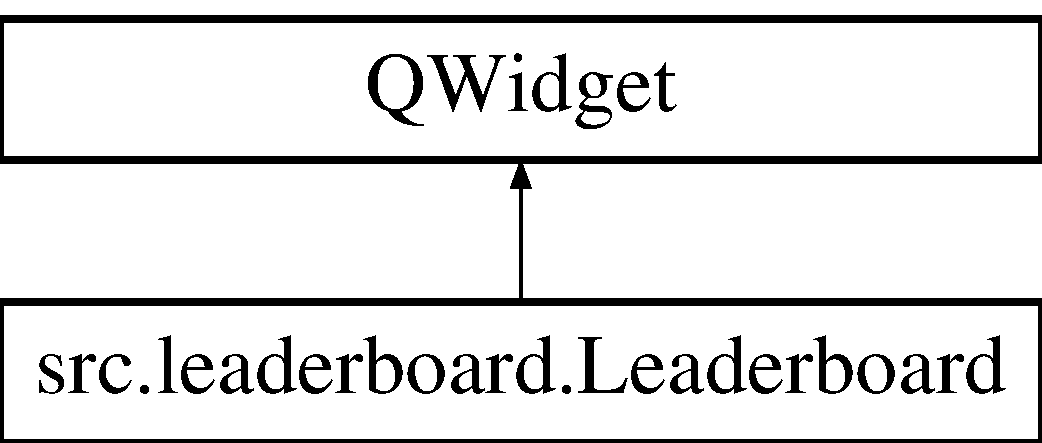
\includegraphics[height=2.000000cm]{classsrc_1_1leaderboard_1_1_leaderboard}
\end{center}
\end{figure}
\subsection*{Public Member Functions}
\begin{DoxyCompactItemize}
\item 
\hypertarget{classsrc_1_1leaderboard_1_1_leaderboard_a7455e00826b66e77d6d56d0970af18b5}{}def {\bfseries \+\_\+\+\_\+init\+\_\+\+\_\+} (self, parent, \hyperlink{classsrc_1_1leaderboard_1_1_leaderboard_abca7271f8092bb5672bf66c04971e04e}{previous\+Menu})\label{classsrc_1_1leaderboard_1_1_leaderboard_a7455e00826b66e77d6d56d0970af18b5}

\item 
def \hyperlink{classsrc_1_1leaderboard_1_1_leaderboard_ad5925cc40678e00c529938ee5105d833}{init\+U\+I} (self)
\begin{DoxyCompactList}\small\item\em this method initiaze the G\+U\+I of the leaderboard. \end{DoxyCompactList}\item 
def \hyperlink{classsrc_1_1leaderboard_1_1_leaderboard_a0cf6394bf691c593a05dadf3969536ba}{fill\+Data} (self)
\begin{DoxyCompactList}\small\item\em this methods fills the data in the table. \end{DoxyCompactList}\item 
def \hyperlink{classsrc_1_1leaderboard_1_1_leaderboard_ade0e52e1b6809df57ea4b1a167c0257b}{back} (self)
\begin{DoxyCompactList}\small\item\em emit back\+Signal when called. \end{DoxyCompactList}\end{DoxyCompactItemize}
\subsection*{Public Attributes}
\begin{DoxyCompactItemize}
\item 
\hyperlink{classsrc_1_1leaderboard_1_1_leaderboard_abca7271f8092bb5672bf66c04971e04e}{previous\+Menu}
\begin{DoxyCompactList}\small\item\em int used to keep track of the previous menu. \end{DoxyCompactList}\item 
\hyperlink{classsrc_1_1leaderboard_1_1_leaderboard_aa059323abc817556528ae54dd5dbca6b}{db}
\begin{DoxyCompactList}\small\item\em instance of the database. \end{DoxyCompactList}\item 
\hyperlink{classsrc_1_1leaderboard_1_1_leaderboard_a48b819acfb54637e30e709361ed32a85}{row\+Count}
\begin{DoxyCompactList}\small\item\em the number of rows is set to 10. \end{DoxyCompactList}\item 
\hypertarget{classsrc_1_1leaderboard_1_1_leaderboard_ac02b975859a4e3cb57eabe5206808a46}{}\hyperlink{classsrc_1_1leaderboard_1_1_leaderboard_ac02b975859a4e3cb57eabe5206808a46}{col\+Count}\label{classsrc_1_1leaderboard_1_1_leaderboard_ac02b975859a4e3cb57eabe5206808a46}

\begin{DoxyCompactList}\small\item\em the number of columns is set to 5 \end{DoxyCompactList}\item 
\hyperlink{classsrc_1_1leaderboard_1_1_leaderboard_a1d9b33cb94b8636038320f10d3d2fe30}{table}
\begin{DoxyCompactList}\small\item\em Is a table of 5 columns (col\+Count) and 10 rows (row\+Count) which contains the top 10 scores. \end{DoxyCompactList}\end{DoxyCompactItemize}
\subsection*{Static Public Attributes}
\begin{DoxyCompactItemize}
\item 
tuple \hyperlink{classsrc_1_1leaderboard_1_1_leaderboard_a8c170d23c0124efb4c1d885720c926af}{back\+Signal} = Qt\+Core.\+pyqt\+Signal(int)
\begin{DoxyCompactList}\small\item\em Signal which will be used to go back to the previous menu based on an int. \end{DoxyCompactList}\end{DoxyCompactItemize}


\subsection{Detailed Description}
This class is a widget that displays the leader\+Board. 

It includes the following buttons and fields that the user can interact with\+:~\newline
table\+: is a field that contains the top 10 players sorted by cumulative scores. back\+Button\+: emit back\+Signal when clicked. 

\subsection{Member Function Documentation}
\hypertarget{classsrc_1_1leaderboard_1_1_leaderboard_ade0e52e1b6809df57ea4b1a167c0257b}{}\index{src\+::leaderboard\+::\+Leaderboard@{src\+::leaderboard\+::\+Leaderboard}!back@{back}}
\index{back@{back}!src\+::leaderboard\+::\+Leaderboard@{src\+::leaderboard\+::\+Leaderboard}}
\subsubsection[{back}]{\setlength{\rightskip}{0pt plus 5cm}def src.\+leaderboard.\+Leaderboard.\+back (
\begin{DoxyParamCaption}
\item[{}]{self}
\end{DoxyParamCaption}
)}\label{classsrc_1_1leaderboard_1_1_leaderboard_ade0e52e1b6809df57ea4b1a167c0257b}


emit back\+Signal when called. 

\hypertarget{classsrc_1_1leaderboard_1_1_leaderboard_a0cf6394bf691c593a05dadf3969536ba}{}\index{src\+::leaderboard\+::\+Leaderboard@{src\+::leaderboard\+::\+Leaderboard}!fill\+Data@{fill\+Data}}
\index{fill\+Data@{fill\+Data}!src\+::leaderboard\+::\+Leaderboard@{src\+::leaderboard\+::\+Leaderboard}}
\subsubsection[{fill\+Data}]{\setlength{\rightskip}{0pt plus 5cm}def src.\+leaderboard.\+Leaderboard.\+fill\+Data (
\begin{DoxyParamCaption}
\item[{}]{self}
\end{DoxyParamCaption}
)}\label{classsrc_1_1leaderboard_1_1_leaderboard_a0cf6394bf691c593a05dadf3969536ba}


this methods fills the data in the table. 

users\+: contains top 10 players sorted by cumulative scores. \hypertarget{classsrc_1_1leaderboard_1_1_leaderboard_ad5925cc40678e00c529938ee5105d833}{}\index{src\+::leaderboard\+::\+Leaderboard@{src\+::leaderboard\+::\+Leaderboard}!init\+U\+I@{init\+U\+I}}
\index{init\+U\+I@{init\+U\+I}!src\+::leaderboard\+::\+Leaderboard@{src\+::leaderboard\+::\+Leaderboard}}
\subsubsection[{init\+U\+I}]{\setlength{\rightskip}{0pt plus 5cm}def src.\+leaderboard.\+Leaderboard.\+init\+U\+I (
\begin{DoxyParamCaption}
\item[{}]{self}
\end{DoxyParamCaption}
)}\label{classsrc_1_1leaderboard_1_1_leaderboard_ad5925cc40678e00c529938ee5105d833}


this method initiaze the G\+U\+I of the leaderboard. 



\subsection{Member Data Documentation}
\hypertarget{classsrc_1_1leaderboard_1_1_leaderboard_a8c170d23c0124efb4c1d885720c926af}{}\index{src\+::leaderboard\+::\+Leaderboard@{src\+::leaderboard\+::\+Leaderboard}!back\+Signal@{back\+Signal}}
\index{back\+Signal@{back\+Signal}!src\+::leaderboard\+::\+Leaderboard@{src\+::leaderboard\+::\+Leaderboard}}
\subsubsection[{back\+Signal}]{\setlength{\rightskip}{0pt plus 5cm}tuple src.\+leaderboard.\+Leaderboard.\+back\+Signal = Qt\+Core.\+pyqt\+Signal(int)\hspace{0.3cm}{\ttfamily [static]}}\label{classsrc_1_1leaderboard_1_1_leaderboard_a8c170d23c0124efb4c1d885720c926af}


Signal which will be used to go back to the previous menu based on an int. 

int is set as \textquotesingle{}previous\+Menu\textquotesingle{} \hypertarget{classsrc_1_1leaderboard_1_1_leaderboard_aa059323abc817556528ae54dd5dbca6b}{}\index{src\+::leaderboard\+::\+Leaderboard@{src\+::leaderboard\+::\+Leaderboard}!db@{db}}
\index{db@{db}!src\+::leaderboard\+::\+Leaderboard@{src\+::leaderboard\+::\+Leaderboard}}
\subsubsection[{db}]{\setlength{\rightskip}{0pt plus 5cm}src.\+leaderboard.\+Leaderboard.\+db}\label{classsrc_1_1leaderboard_1_1_leaderboard_aa059323abc817556528ae54dd5dbca6b}


instance of the database. 

\hypertarget{classsrc_1_1leaderboard_1_1_leaderboard_abca7271f8092bb5672bf66c04971e04e}{}\index{src\+::leaderboard\+::\+Leaderboard@{src\+::leaderboard\+::\+Leaderboard}!previous\+Menu@{previous\+Menu}}
\index{previous\+Menu@{previous\+Menu}!src\+::leaderboard\+::\+Leaderboard@{src\+::leaderboard\+::\+Leaderboard}}
\subsubsection[{previous\+Menu}]{\setlength{\rightskip}{0pt plus 5cm}src.\+leaderboard.\+Leaderboard.\+previous\+Menu}\label{classsrc_1_1leaderboard_1_1_leaderboard_abca7271f8092bb5672bf66c04971e04e}


int used to keep track of the previous menu. 

\hypertarget{classsrc_1_1leaderboard_1_1_leaderboard_a48b819acfb54637e30e709361ed32a85}{}\index{src\+::leaderboard\+::\+Leaderboard@{src\+::leaderboard\+::\+Leaderboard}!row\+Count@{row\+Count}}
\index{row\+Count@{row\+Count}!src\+::leaderboard\+::\+Leaderboard@{src\+::leaderboard\+::\+Leaderboard}}
\subsubsection[{row\+Count}]{\setlength{\rightskip}{0pt plus 5cm}src.\+leaderboard.\+Leaderboard.\+row\+Count}\label{classsrc_1_1leaderboard_1_1_leaderboard_a48b819acfb54637e30e709361ed32a85}


the number of rows is set to 10. 

\hypertarget{classsrc_1_1leaderboard_1_1_leaderboard_a1d9b33cb94b8636038320f10d3d2fe30}{}\index{src\+::leaderboard\+::\+Leaderboard@{src\+::leaderboard\+::\+Leaderboard}!table@{table}}
\index{table@{table}!src\+::leaderboard\+::\+Leaderboard@{src\+::leaderboard\+::\+Leaderboard}}
\subsubsection[{table}]{\setlength{\rightskip}{0pt plus 5cm}src.\+leaderboard.\+Leaderboard.\+table}\label{classsrc_1_1leaderboard_1_1_leaderboard_a1d9b33cb94b8636038320f10d3d2fe30}


Is a table of 5 columns (col\+Count) and 10 rows (row\+Count) which contains the top 10 scores. 



The documentation for this class was generated from the following file\+:\begin{DoxyCompactItemize}
\item 
src/leaderboard.\+py\end{DoxyCompactItemize}

\hypertarget{classsrc_1_1level_1_1_level}{}\section{src.\+level.\+Level Class Reference}
\label{classsrc_1_1level_1_1_level}\index{src.\+level.\+Level@{src.\+level.\+Level}}


\hyperlink{classsrc_1_1level_1_1_level}{Level} object containing all the attributes and methods necessary to one level of gameplay.  


Inheritance diagram for src.\+level.\+Level\+:\begin{figure}[H]
\begin{center}
\leavevmode
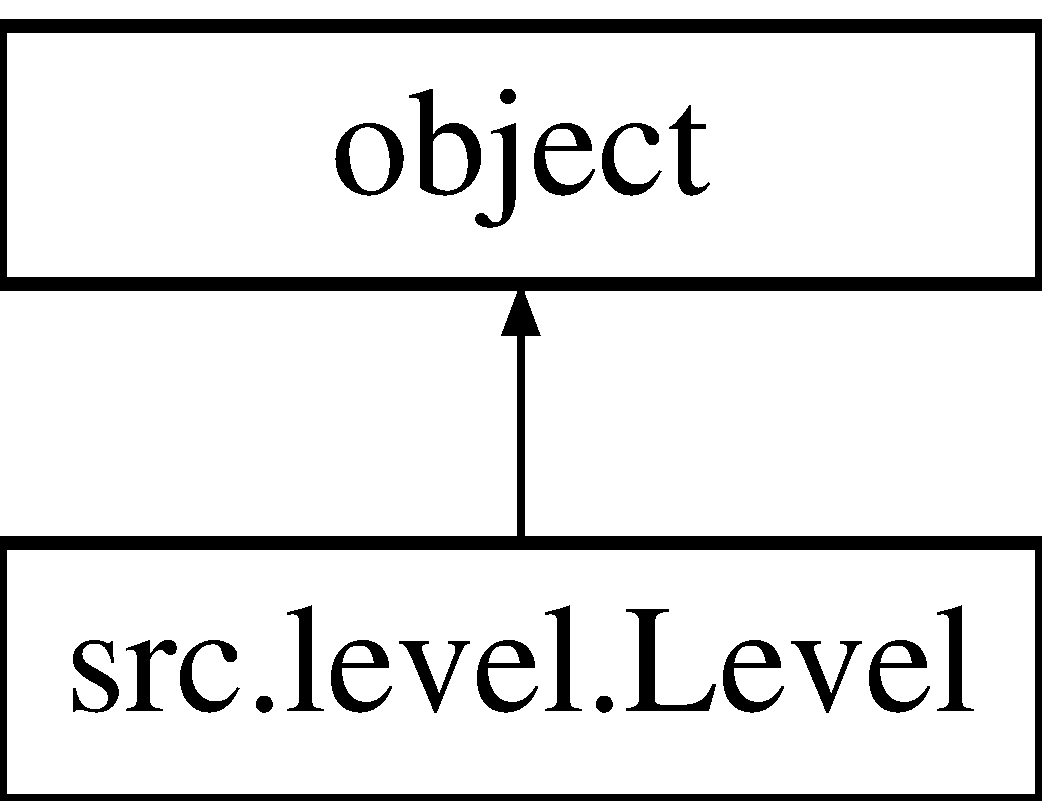
\includegraphics[height=2.000000cm]{classsrc_1_1level_1_1_level}
\end{center}
\end{figure}
\subsection*{Public Member Functions}
\begin{DoxyCompactItemize}
\item 
\hypertarget{classsrc_1_1level_1_1_level_ab6e52c74e02be818576be2ffd9040fe0}{}def \hyperlink{classsrc_1_1level_1_1_level_ab6e52c74e02be818576be2ffd9040fe0}{\+\_\+\+\_\+init\+\_\+\+\_\+} (self, \hyperlink{classsrc_1_1level_1_1_level_a7ec8be181d4558bc3f7b8c106a6aeb5a}{username}, \hyperlink{classsrc_1_1level_1_1_level_a8b26c1249a2d161c058595e789948bf9}{level\+Num})\label{classsrc_1_1level_1_1_level_ab6e52c74e02be818576be2ffd9040fe0}

\begin{DoxyCompactList}\small\item\em Constructor of a level which takes a username and a level as argument. \end{DoxyCompactList}\item 
\hypertarget{classsrc_1_1level_1_1_level_a0df76bcc440bbab23e4ce754223177c5}{}def \hyperlink{classsrc_1_1level_1_1_level_a0df76bcc440bbab23e4ce754223177c5}{set\+New\+Level} (self)\label{classsrc_1_1level_1_1_level_a0df76bcc440bbab23e4ce754223177c5}

\begin{DoxyCompactList}\small\item\em Reinitialize all of level\textquotesingle{}s variables and bomberman\textquotesingle{}s variable to start new level. \end{DoxyCompactList}\item 
\hypertarget{classsrc_1_1level_1_1_level_a9af98db5112ae2fbd4a9f44ae0bcbe83}{}def \hyperlink{classsrc_1_1level_1_1_level_a9af98db5112ae2fbd4a9f44ae0bcbe83}{gain\+Power\+Up} (self)\label{classsrc_1_1level_1_1_level_a9af98db5112ae2fbd4a9f44ae0bcbe83}

\begin{DoxyCompactList}\small\item\em This method activates the current level\textquotesingle{}s powerup and add attribute to bomberman. \end{DoxyCompactList}\item 
\hypertarget{classsrc_1_1level_1_1_level_a9f1a64a223be266425f6100e4728df3a}{}def \hyperlink{classsrc_1_1level_1_1_level_a9f1a64a223be266425f6100e4728df3a}{tile\+At} (self, x, y)\label{classsrc_1_1level_1_1_level_a9f1a64a223be266425f6100e4728df3a}

\begin{DoxyCompactList}\small\item\em This method returns the tile at x and y from the board. \end{DoxyCompactList}\item 
\hypertarget{classsrc_1_1level_1_1_level_a1b0a565e03f055cd93abe6faeefd3b4f}{}def \hyperlink{classsrc_1_1level_1_1_level_a1b0a565e03f055cd93abe6faeefd3b4f}{set\+Tile\+At} (self, x, y, tile)\label{classsrc_1_1level_1_1_level_a1b0a565e03f055cd93abe6faeefd3b4f}

\begin{DoxyCompactList}\small\item\em This method sets tile at x and y on the board. \end{DoxyCompactList}\item 
\hypertarget{classsrc_1_1level_1_1_level_a79a922117841f374126a4ab727a65ef1}{}def \hyperlink{classsrc_1_1level_1_1_level_a79a922117841f374126a4ab727a65ef1}{pop\+Tile\+At} (self, x, y)\label{classsrc_1_1level_1_1_level_a79a922117841f374126a4ab727a65ef1}

\begin{DoxyCompactList}\small\item\em This method removes the tile at x and y from the board. \end{DoxyCompactList}\item 
\hypertarget{classsrc_1_1level_1_1_level_aa1fdbf2a27cb66fffd27bc2598449072}{}def \hyperlink{classsrc_1_1level_1_1_level_aa1fdbf2a27cb66fffd27bc2598449072}{set\+Bomb} (self)\label{classsrc_1_1level_1_1_level_aa1fdbf2a27cb66fffd27bc2598449072}

\begin{DoxyCompactList}\small\item\em This method lays a bomb at bomberman\textquotesingle{}s current position. \end{DoxyCompactList}\item 
\hypertarget{classsrc_1_1level_1_1_level_ab1083324efb6eddfdfc04316a85f7f15}{}def \hyperlink{classsrc_1_1level_1_1_level_ab1083324efb6eddfdfc04316a85f7f15}{clear\+Board} (self)\label{classsrc_1_1level_1_1_level_ab1083324efb6eddfdfc04316a85f7f15}

\begin{DoxyCompactList}\small\item\em This method clears all tiles on the board. \end{DoxyCompactList}\item 
\hypertarget{classsrc_1_1level_1_1_level_a5cacfb3b893af155c71dfffc3ae042bd}{}def \hyperlink{classsrc_1_1level_1_1_level_a5cacfb3b893af155c71dfffc3ae042bd}{clear\+Bombs} (self)\label{classsrc_1_1level_1_1_level_a5cacfb3b893af155c71dfffc3ae042bd}

\begin{DoxyCompactList}\small\item\em This method clears all bombs from the bomb queue. \end{DoxyCompactList}\item 
\hypertarget{classsrc_1_1level_1_1_level_ad43e3dab276d7ea38b268f22827b0236}{}def \hyperlink{classsrc_1_1level_1_1_level_ad43e3dab276d7ea38b268f22827b0236}{set\+Concrete} (self)\label{classsrc_1_1level_1_1_level_ad43e3dab276d7ea38b268f22827b0236}

\begin{DoxyCompactList}\small\item\em This method sets concrete tiles systematically on the board. \end{DoxyCompactList}\item 
\hypertarget{classsrc_1_1level_1_1_level_a37d135e2fd7961eb5f2921447d1c8243}{}def \hyperlink{classsrc_1_1level_1_1_level_a37d135e2fd7961eb5f2921447d1c8243}{set\+Exit} (self)\label{classsrc_1_1level_1_1_level_a37d135e2fd7961eb5f2921447d1c8243}

\begin{DoxyCompactList}\small\item\em This method sets an exit tile randomly on the board and set a brick on top of it. \end{DoxyCompactList}\item 
\hypertarget{classsrc_1_1level_1_1_level_a6e5e52649e074784152f5fe8f94ded08}{}def \hyperlink{classsrc_1_1level_1_1_level_a6e5e52649e074784152f5fe8f94ded08}{set\+Level\+Info} (self)\label{classsrc_1_1level_1_1_level_a6e5e52649e074784152f5fe8f94ded08}

\begin{DoxyCompactList}\small\item\em This method fetches a the list of enemies and powerup matching the current level number. \end{DoxyCompactList}\item 
\hypertarget{classsrc_1_1level_1_1_level_a7ab32312eb682ecce07ae83551c051e1}{}def \hyperlink{classsrc_1_1level_1_1_level_a7ab32312eb682ecce07ae83551c051e1}{set\+Powerup} (self)\label{classsrc_1_1level_1_1_level_a7ab32312eb682ecce07ae83551c051e1}

\begin{DoxyCompactList}\small\item\em This method sets a powerup tile randomly on the board and set a brick on top of it. \end{DoxyCompactList}\item 
\hypertarget{classsrc_1_1level_1_1_level_ae430589f114a19e13c2667e8ef37e266}{}def \hyperlink{classsrc_1_1level_1_1_level_ae430589f114a19e13c2667e8ef37e266}{set\+Brick} (self)\label{classsrc_1_1level_1_1_level_ae430589f114a19e13c2667e8ef37e266}

\begin{DoxyCompactList}\small\item\em This method sets brick tiles randomly on the board. \end{DoxyCompactList}\item 
\hypertarget{classsrc_1_1level_1_1_level_a76cfaab350e8f7699f054e9e9423de6c}{}def \hyperlink{classsrc_1_1level_1_1_level_a76cfaab350e8f7699f054e9e9423de6c}{set\+Bomberman} (self)\label{classsrc_1_1level_1_1_level_a76cfaab350e8f7699f054e9e9423de6c}

\begin{DoxyCompactList}\small\item\em This method sets bomberman at x and y on the board. \end{DoxyCompactList}\item 
\hypertarget{classsrc_1_1level_1_1_level_af60d85055b9f07935312e581b5316364}{}def \hyperlink{classsrc_1_1level_1_1_level_af60d85055b9f07935312e581b5316364}{set\+Enemies} (self)\label{classsrc_1_1level_1_1_level_af60d85055b9f07935312e581b5316364}

\begin{DoxyCompactList}\small\item\em This method sets enemies randomly on the map. \end{DoxyCompactList}\item 
\hypertarget{classsrc_1_1level_1_1_level_acd226ddc877d5bf1e18c4d2a7e790fb3}{}def \hyperlink{classsrc_1_1level_1_1_level_acd226ddc877d5bf1e18c4d2a7e790fb3}{clear\+Enemies} (self)\label{classsrc_1_1level_1_1_level_acd226ddc877d5bf1e18c4d2a7e790fb3}

\begin{DoxyCompactList}\small\item\em This method clears all enemies on the map and in the list of enemies and list of enemies type. \end{DoxyCompactList}\item 
\hypertarget{classsrc_1_1level_1_1_level_a4b318116c4f5b2bdad46be495e21c53d}{}def \hyperlink{classsrc_1_1level_1_1_level_a4b318116c4f5b2bdad46be495e21c53d}{set\+Chaos} (self)\label{classsrc_1_1level_1_1_level_a4b318116c4f5b2bdad46be495e21c53d}

\begin{DoxyCompactList}\small\item\em This method sets 8 mega enemies everywhere, used when bomb detonates an exit tile or powerup tile. \end{DoxyCompactList}\item 
\hypertarget{classsrc_1_1level_1_1_level_acf03686c3657b7e1a5436bbf1b721bf2}{}def \hyperlink{classsrc_1_1level_1_1_level_acf03686c3657b7e1a5436bbf1b721bf2}{set\+Super\+Chaos} (self)\label{classsrc_1_1level_1_1_level_acf03686c3657b7e1a5436bbf1b721bf2}

\begin{DoxyCompactList}\small\item\em This method sets 8 maximum level enemies everywhere. \end{DoxyCompactList}\end{DoxyCompactItemize}
\subsection*{Public Attributes}
\begin{DoxyCompactItemize}
\item 
\hypertarget{classsrc_1_1level_1_1_level_a07cb236f1acaa42ea5ad2c20fec75c3b}{}\hyperlink{classsrc_1_1level_1_1_level_a07cb236f1acaa42ea5ad2c20fec75c3b}{bomberman}\label{classsrc_1_1level_1_1_level_a07cb236f1acaa42ea5ad2c20fec75c3b}

\begin{DoxyCompactList}\small\item\em Initialize bomberman. \end{DoxyCompactList}\item 
\hypertarget{classsrc_1_1level_1_1_level_a7ec8be181d4558bc3f7b8c106a6aeb5a}{}\hyperlink{classsrc_1_1level_1_1_level_a7ec8be181d4558bc3f7b8c106a6aeb5a}{username}\label{classsrc_1_1level_1_1_level_a7ec8be181d4558bc3f7b8c106a6aeb5a}

\begin{DoxyCompactList}\small\item\em String Player\textquotesingle{}s username. \end{DoxyCompactList}\item 
\hypertarget{classsrc_1_1level_1_1_level_a8b26c1249a2d161c058595e789948bf9}{}\hyperlink{classsrc_1_1level_1_1_level_a8b26c1249a2d161c058595e789948bf9}{level\+Num}\label{classsrc_1_1level_1_1_level_a8b26c1249a2d161c058595e789948bf9}

\begin{DoxyCompactList}\small\item\em Integer the level\textquotesingle{}s number. \end{DoxyCompactList}\item 
\hypertarget{classsrc_1_1level_1_1_level_a65841b782b1342d40aa32c3a788cf6b0}{}\hyperlink{classsrc_1_1level_1_1_level_a65841b782b1342d40aa32c3a788cf6b0}{is\+Initialized}\label{classsrc_1_1level_1_1_level_a65841b782b1342d40aa32c3a788cf6b0}

\begin{DoxyCompactList}\small\item\em Boolean True if the game has started. \end{DoxyCompactList}\item 
\hypertarget{classsrc_1_1level_1_1_level_aa09aade96eec6dbcdf4b04754a3fcf17}{}\hyperlink{classsrc_1_1level_1_1_level_aa09aade96eec6dbcdf4b04754a3fcf17}{board}\label{classsrc_1_1level_1_1_level_aa09aade96eec6dbcdf4b04754a3fcf17}

\begin{DoxyCompactList}\small\item\em Nested List of Tile(s) representing the game board. \end{DoxyCompactList}\item 
\hypertarget{classsrc_1_1level_1_1_level_ad6cc50ff3008c2fd8497b22070d7da64}{}\hyperlink{classsrc_1_1level_1_1_level_ad6cc50ff3008c2fd8497b22070d7da64}{bomb\+Queue}\label{classsrc_1_1level_1_1_level_ad6cc50ff3008c2fd8497b22070d7da64}

\begin{DoxyCompactList}\small\item\em Queue containing the coords and time left of bombs laid by bomberman. \end{DoxyCompactList}\item 
\hypertarget{classsrc_1_1level_1_1_level_ac6d2065a5cd3ddd4348bb7f6394a0b46}{}\hyperlink{classsrc_1_1level_1_1_level_ac6d2065a5cd3ddd4348bb7f6394a0b46}{flash\+Queue}\label{classsrc_1_1level_1_1_level_ac6d2065a5cd3ddd4348bb7f6394a0b46}

\begin{DoxyCompactList}\small\item\em Queue containing the coords and time left of flame tiles produced by bomb(s) \end{DoxyCompactList}\item 
\hypertarget{classsrc_1_1level_1_1_level_a5445bee2b7b93a1caa1a0a5bf3455db9}{}\hyperlink{classsrc_1_1level_1_1_level_a5445bee2b7b93a1caa1a0a5bf3455db9}{power\+Up\+Coord}\label{classsrc_1_1level_1_1_level_a5445bee2b7b93a1caa1a0a5bf3455db9}

\begin{DoxyCompactList}\small\item\em List coordinates of the powerup tile. \end{DoxyCompactList}\item 
\hypertarget{classsrc_1_1level_1_1_level_ab0595b7e689e25d540f0f486413e0514}{}\hyperlink{classsrc_1_1level_1_1_level_ab0595b7e689e25d540f0f486413e0514}{exit\+Coord}\label{classsrc_1_1level_1_1_level_ab0595b7e689e25d540f0f486413e0514}

\begin{DoxyCompactList}\small\item\em List coordinates of the exit tile. \end{DoxyCompactList}\item 
\hypertarget{classsrc_1_1level_1_1_level_a50126ed45ccd7be41b5b80a4bf821028}{}\hyperlink{classsrc_1_1level_1_1_level_a50126ed45ccd7be41b5b80a4bf821028}{power\+Up}\label{classsrc_1_1level_1_1_level_a50126ed45ccd7be41b5b80a4bf821028}

\begin{DoxyCompactList}\small\item\em Integer type of powerup. \end{DoxyCompactList}\item 
\hypertarget{classsrc_1_1level_1_1_level_a0a652366b9fe32851d20915af1dbc0f3}{}\hyperlink{classsrc_1_1level_1_1_level_a0a652366b9fe32851d20915af1dbc0f3}{number\+Enemies}\label{classsrc_1_1level_1_1_level_a0a652366b9fe32851d20915af1dbc0f3}

\begin{DoxyCompactList}\small\item\em Integer number of enemies in the board. \end{DoxyCompactList}\item 
\hypertarget{classsrc_1_1level_1_1_level_ad45aaceea3034ea0e83e1627a47ea2d2}{}\hyperlink{classsrc_1_1level_1_1_level_ad45aaceea3034ea0e83e1627a47ea2d2}{list\+Enemies}\label{classsrc_1_1level_1_1_level_ad45aaceea3034ea0e83e1627a47ea2d2}

\begin{DoxyCompactList}\small\item\em List of all enemies in the board. \end{DoxyCompactList}\item 
\hyperlink{classsrc_1_1level_1_1_level_a198d86791a4f4a570909d80490057ae9}{list\+Type\+Enemies}
\begin{DoxyCompactList}\small\item\em List of Integer all enemies by type, e.\+g. \end{DoxyCompactList}\item 
\hypertarget{classsrc_1_1level_1_1_level_a0272ba87f68c6b056d20751096f576d9}{}\hyperlink{classsrc_1_1level_1_1_level_a0272ba87f68c6b056d20751096f576d9}{time\+Left}\label{classsrc_1_1level_1_1_level_a0272ba87f68c6b056d20751096f576d9}

\begin{DoxyCompactList}\small\item\em Integer time left in the game. \end{DoxyCompactList}\item 
\hypertarget{classsrc_1_1level_1_1_level_aec7becdb4db743d76dbb993cb22a22bb}{}\hyperlink{classsrc_1_1level_1_1_level_aec7becdb4db743d76dbb993cb22a22bb}{time\+Done}\label{classsrc_1_1level_1_1_level_aec7becdb4db743d76dbb993cb22a22bb}

\begin{DoxyCompactList}\small\item\em Boolean True if time has elapsed. \end{DoxyCompactList}\item 
\hypertarget{classsrc_1_1level_1_1_level_a91123ee7d794996b5504dcb8550f7684}{}\hyperlink{classsrc_1_1level_1_1_level_a91123ee7d794996b5504dcb8550f7684}{score}\label{classsrc_1_1level_1_1_level_a91123ee7d794996b5504dcb8550f7684}

\begin{DoxyCompactList}\small\item\em Integer player\textquotesingle{}s score. \end{DoxyCompactList}\end{DoxyCompactItemize}


\subsection{Detailed Description}
\hyperlink{classsrc_1_1level_1_1_level}{Level} object containing all the attributes and methods necessary to one level of gameplay. 

\subsection{Member Data Documentation}
\hypertarget{classsrc_1_1level_1_1_level_a198d86791a4f4a570909d80490057ae9}{}\index{src\+::level\+::\+Level@{src\+::level\+::\+Level}!list\+Type\+Enemies@{list\+Type\+Enemies}}
\index{list\+Type\+Enemies@{list\+Type\+Enemies}!src\+::level\+::\+Level@{src\+::level\+::\+Level}}
\subsubsection[{list\+Type\+Enemies}]{\setlength{\rightskip}{0pt plus 5cm}src.\+level.\+Level.\+list\+Type\+Enemies}\label{classsrc_1_1level_1_1_level_a198d86791a4f4a570909d80490057ae9}


List of Integer all enemies by type, e.\+g. 

value at index 0 represents the number of enemies of level 0 

The documentation for this class was generated from the following file\+:\begin{DoxyCompactItemize}
\item 
src/level.\+py\end{DoxyCompactItemize}

\hypertarget{classsrc_1_1level__menu_1_1_level_menu}{}\section{src.\+level\+\_\+menu.\+Level\+Menu Class Reference}
\label{classsrc_1_1level__menu_1_1_level_menu}\index{src.\+level\+\_\+menu.\+Level\+Menu@{src.\+level\+\_\+menu.\+Level\+Menu}}


This class is a widget that displays the level menu.  


Inheritance diagram for src.\+level\+\_\+menu.\+Level\+Menu\+:\begin{figure}[H]
\begin{center}
\leavevmode
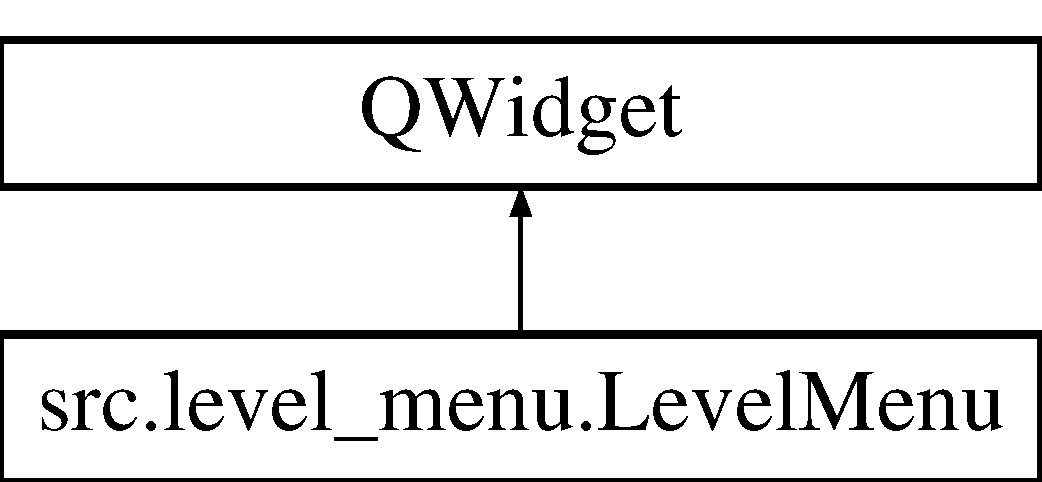
\includegraphics[height=2.000000cm]{classsrc_1_1level__menu_1_1_level_menu}
\end{center}
\end{figure}
\subsection*{Public Member Functions}
\begin{DoxyCompactItemize}
\item 
\hypertarget{classsrc_1_1level__menu_1_1_level_menu_a39fd7912eb9a473b0fb03b5ae1bd0d84}{}def {\bfseries \+\_\+\+\_\+init\+\_\+\+\_\+} (self, parent, \hyperlink{classsrc_1_1level__menu_1_1_level_menu_aee1d2148e23a2908c72c4a8f8ad0a98f}{username})\label{classsrc_1_1level__menu_1_1_level_menu_a39fd7912eb9a473b0fb03b5ae1bd0d84}

\item 
def \hyperlink{classsrc_1_1level__menu_1_1_level_menu_a85ba6c3a92e1f256f70186866f2795ac}{init\+U\+I} (self)
\begin{DoxyCompactList}\small\item\em This method initialize the G\+U\+I of the level menu. \end{DoxyCompactList}\item 
def \hyperlink{classsrc_1_1level__menu_1_1_level_menu_a5852c765b18d5e6c28d5fdb7ebf80427}{back\+To\+Main\+Menu} (self)
\begin{DoxyCompactList}\small\item\em emit back\+To\+Main\+Menu\+Signal when called. \end{DoxyCompactList}\item 
def \hyperlink{classsrc_1_1level__menu_1_1_level_menu_aafc4b32a91edcdf2a10f5de32efbda2a}{start\+Level} (self, level)
\begin{DoxyCompactList}\small\item\em emit start\+Level\+Signal when called. \end{DoxyCompactList}\end{DoxyCompactItemize}
\subsection*{Public Attributes}
\begin{DoxyCompactItemize}
\item 
\hyperlink{classsrc_1_1level__menu_1_1_level_menu_aee1d2148e23a2908c72c4a8f8ad0a98f}{username}
\begin{DoxyCompactList}\small\item\em This is the currently active user\textquotesingle{}s username. \end{DoxyCompactList}\item 
\hyperlink{classsrc_1_1level__menu_1_1_level_menu_a3224111dd78be1b15cc943f41daef0cf}{db}
\begin{DoxyCompactList}\small\item\em Instance of the database. \end{DoxyCompactList}\end{DoxyCompactItemize}
\subsection*{Static Public Attributes}
\begin{DoxyCompactItemize}
\item 
tuple \hyperlink{classsrc_1_1level__menu_1_1_level_menu_a769225d8895542b2c7118110d7b2ff9d}{back\+To\+Main\+Menu\+Signal} = Qt\+Core.\+pyqt\+Signal()
\begin{DoxyCompactList}\small\item\em Signal which will be used to go back to the main menu. \end{DoxyCompactList}\item 
tuple \hyperlink{classsrc_1_1level__menu_1_1_level_menu_a14a5a5bd905bb0d8e732a33bed71ef44}{start\+Level\+Signal} = Qt\+Core.\+pyqt\+Signal(int)
\begin{DoxyCompactList}\small\item\em Signal which will be used to start the game. \end{DoxyCompactList}\end{DoxyCompactItemize}


\subsection{Detailed Description}
This class is a widget that displays the level menu. 

It includes buttons that the user can interact with. 

\subsection{Member Function Documentation}
\hypertarget{classsrc_1_1level__menu_1_1_level_menu_a5852c765b18d5e6c28d5fdb7ebf80427}{}\index{src\+::level\+\_\+menu\+::\+Level\+Menu@{src\+::level\+\_\+menu\+::\+Level\+Menu}!back\+To\+Main\+Menu@{back\+To\+Main\+Menu}}
\index{back\+To\+Main\+Menu@{back\+To\+Main\+Menu}!src\+::level\+\_\+menu\+::\+Level\+Menu@{src\+::level\+\_\+menu\+::\+Level\+Menu}}
\subsubsection[{back\+To\+Main\+Menu}]{\setlength{\rightskip}{0pt plus 5cm}def src.\+level\+\_\+menu.\+Level\+Menu.\+back\+To\+Main\+Menu (
\begin{DoxyParamCaption}
\item[{}]{self}
\end{DoxyParamCaption}
)}\label{classsrc_1_1level__menu_1_1_level_menu_a5852c765b18d5e6c28d5fdb7ebf80427}


emit back\+To\+Main\+Menu\+Signal when called. 

\hypertarget{classsrc_1_1level__menu_1_1_level_menu_a85ba6c3a92e1f256f70186866f2795ac}{}\index{src\+::level\+\_\+menu\+::\+Level\+Menu@{src\+::level\+\_\+menu\+::\+Level\+Menu}!init\+U\+I@{init\+U\+I}}
\index{init\+U\+I@{init\+U\+I}!src\+::level\+\_\+menu\+::\+Level\+Menu@{src\+::level\+\_\+menu\+::\+Level\+Menu}}
\subsubsection[{init\+U\+I}]{\setlength{\rightskip}{0pt plus 5cm}def src.\+level\+\_\+menu.\+Level\+Menu.\+init\+U\+I (
\begin{DoxyParamCaption}
\item[{}]{self}
\end{DoxyParamCaption}
)}\label{classsrc_1_1level__menu_1_1_level_menu_a85ba6c3a92e1f256f70186866f2795ac}


This method initialize the G\+U\+I of the level menu. 

\hypertarget{classsrc_1_1level__menu_1_1_level_menu_aafc4b32a91edcdf2a10f5de32efbda2a}{}\index{src\+::level\+\_\+menu\+::\+Level\+Menu@{src\+::level\+\_\+menu\+::\+Level\+Menu}!start\+Level@{start\+Level}}
\index{start\+Level@{start\+Level}!src\+::level\+\_\+menu\+::\+Level\+Menu@{src\+::level\+\_\+menu\+::\+Level\+Menu}}
\subsubsection[{start\+Level}]{\setlength{\rightskip}{0pt plus 5cm}def src.\+level\+\_\+menu.\+Level\+Menu.\+start\+Level (
\begin{DoxyParamCaption}
\item[{}]{self, }
\item[{}]{level}
\end{DoxyParamCaption}
)}\label{classsrc_1_1level__menu_1_1_level_menu_aafc4b32a91edcdf2a10f5de32efbda2a}


emit start\+Level\+Signal when called. 



\subsection{Member Data Documentation}
\hypertarget{classsrc_1_1level__menu_1_1_level_menu_a769225d8895542b2c7118110d7b2ff9d}{}\index{src\+::level\+\_\+menu\+::\+Level\+Menu@{src\+::level\+\_\+menu\+::\+Level\+Menu}!back\+To\+Main\+Menu\+Signal@{back\+To\+Main\+Menu\+Signal}}
\index{back\+To\+Main\+Menu\+Signal@{back\+To\+Main\+Menu\+Signal}!src\+::level\+\_\+menu\+::\+Level\+Menu@{src\+::level\+\_\+menu\+::\+Level\+Menu}}
\subsubsection[{back\+To\+Main\+Menu\+Signal}]{\setlength{\rightskip}{0pt plus 5cm}tuple src.\+level\+\_\+menu.\+Level\+Menu.\+back\+To\+Main\+Menu\+Signal = Qt\+Core.\+pyqt\+Signal()\hspace{0.3cm}{\ttfamily [static]}}\label{classsrc_1_1level__menu_1_1_level_menu_a769225d8895542b2c7118110d7b2ff9d}


Signal which will be used to go back to the main menu. 

\hypertarget{classsrc_1_1level__menu_1_1_level_menu_a3224111dd78be1b15cc943f41daef0cf}{}\index{src\+::level\+\_\+menu\+::\+Level\+Menu@{src\+::level\+\_\+menu\+::\+Level\+Menu}!db@{db}}
\index{db@{db}!src\+::level\+\_\+menu\+::\+Level\+Menu@{src\+::level\+\_\+menu\+::\+Level\+Menu}}
\subsubsection[{db}]{\setlength{\rightskip}{0pt plus 5cm}src.\+level\+\_\+menu.\+Level\+Menu.\+db}\label{classsrc_1_1level__menu_1_1_level_menu_a3224111dd78be1b15cc943f41daef0cf}


Instance of the database. 

\hypertarget{classsrc_1_1level__menu_1_1_level_menu_a14a5a5bd905bb0d8e732a33bed71ef44}{}\index{src\+::level\+\_\+menu\+::\+Level\+Menu@{src\+::level\+\_\+menu\+::\+Level\+Menu}!start\+Level\+Signal@{start\+Level\+Signal}}
\index{start\+Level\+Signal@{start\+Level\+Signal}!src\+::level\+\_\+menu\+::\+Level\+Menu@{src\+::level\+\_\+menu\+::\+Level\+Menu}}
\subsubsection[{start\+Level\+Signal}]{\setlength{\rightskip}{0pt plus 5cm}tuple src.\+level\+\_\+menu.\+Level\+Menu.\+start\+Level\+Signal = Qt\+Core.\+pyqt\+Signal(int)\hspace{0.3cm}{\ttfamily [static]}}\label{classsrc_1_1level__menu_1_1_level_menu_a14a5a5bd905bb0d8e732a33bed71ef44}


Signal which will be used to start the game. 

Integer is the number representing the level chosen by the user. \hypertarget{classsrc_1_1level__menu_1_1_level_menu_aee1d2148e23a2908c72c4a8f8ad0a98f}{}\index{src\+::level\+\_\+menu\+::\+Level\+Menu@{src\+::level\+\_\+menu\+::\+Level\+Menu}!username@{username}}
\index{username@{username}!src\+::level\+\_\+menu\+::\+Level\+Menu@{src\+::level\+\_\+menu\+::\+Level\+Menu}}
\subsubsection[{username}]{\setlength{\rightskip}{0pt plus 5cm}src.\+level\+\_\+menu.\+Level\+Menu.\+username}\label{classsrc_1_1level__menu_1_1_level_menu_aee1d2148e23a2908c72c4a8f8ad0a98f}


This is the currently active user\textquotesingle{}s username. 



The documentation for this class was generated from the following file\+:\begin{DoxyCompactItemize}
\item 
src/level\+\_\+menu.\+py\end{DoxyCompactItemize}

\hypertarget{classsrc_1_1load__menu_1_1_load_menu}{}\section{src.\+load\+\_\+menu.\+Load\+Menu Class Reference}
\label{classsrc_1_1load__menu_1_1_load_menu}\index{src.\+load\+\_\+menu.\+Load\+Menu@{src.\+load\+\_\+menu.\+Load\+Menu}}


This class is a widget that displays the Load menu.  


Inheritance diagram for src.\+load\+\_\+menu.\+Load\+Menu\+:\begin{figure}[H]
\begin{center}
\leavevmode
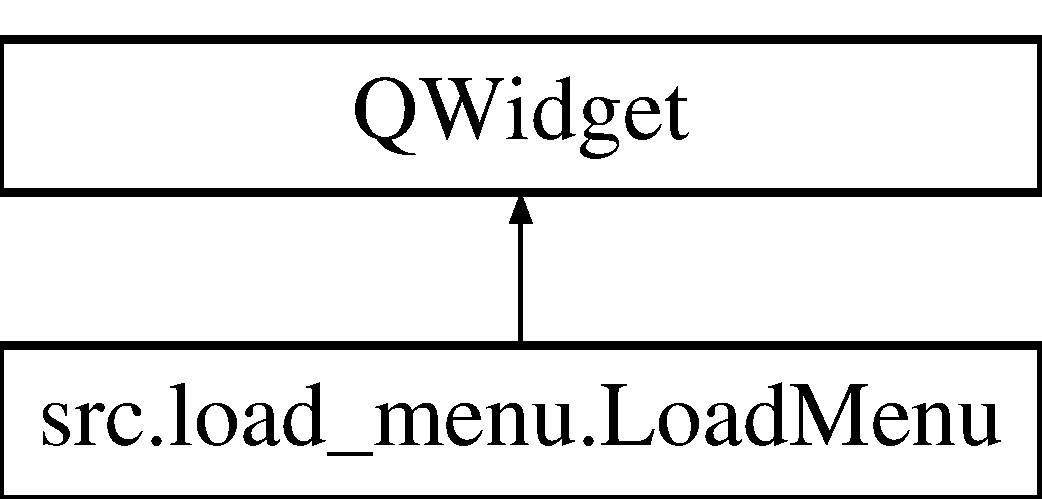
\includegraphics[height=2.000000cm]{classsrc_1_1load__menu_1_1_load_menu}
\end{center}
\end{figure}
\subsection*{Public Member Functions}
\begin{DoxyCompactItemize}
\item 
\hypertarget{classsrc_1_1load__menu_1_1_load_menu_a6b067e9ede752fd13ed4df84570083b7}{}def {\bfseries \+\_\+\+\_\+init\+\_\+\+\_\+} (self, parent, \hyperlink{classsrc_1_1load__menu_1_1_load_menu_ab1c940f6352015a62d85b668bc6ebb01}{username}, \hyperlink{classsrc_1_1load__menu_1_1_load_menu_a266279b7ed3e68889b07c1785251c806}{previous\+Menu})\label{classsrc_1_1load__menu_1_1_load_menu_a6b067e9ede752fd13ed4df84570083b7}

\item 
def \hyperlink{classsrc_1_1load__menu_1_1_load_menu_ae10c4104f4245eaba4772a7f29485ff4}{init\+U\+I} (self)
\begin{DoxyCompactList}\small\item\em This method initialize the G\+U\+I of the Load menu. \end{DoxyCompactList}\item 
def \hyperlink{classsrc_1_1load__menu_1_1_load_menu_ac3ab22ee56c51e7cb02f27344d6bfcbd}{load\+Saved\+Game} (self)
\begin{DoxyCompactList}\small\item\em emit load\+Saved\+Game\+Signal when called. \end{DoxyCompactList}\item 
def \hyperlink{classsrc_1_1load__menu_1_1_load_menu_af7b9c789c68fb85b2d4e2bfd211e201d}{load\+Saved\+Game\+List} (self)
\begin{DoxyCompactList}\small\item\em fetch from the database the current user\textquotesingle{}s saved game. \end{DoxyCompactList}\item 
def \hyperlink{classsrc_1_1load__menu_1_1_load_menu_ac1756d59b9d5d3c026d4cb971bb6a657}{back} (self)
\begin{DoxyCompactList}\small\item\em emit back\+Signal when called. \end{DoxyCompactList}\end{DoxyCompactItemize}
\subsection*{Public Attributes}
\begin{DoxyCompactItemize}
\item 
\hypertarget{classsrc_1_1load__menu_1_1_load_menu_a266279b7ed3e68889b07c1785251c806}{}\hyperlink{classsrc_1_1load__menu_1_1_load_menu_a266279b7ed3e68889b07c1785251c806}{previous\+Menu}\label{classsrc_1_1load__menu_1_1_load_menu_a266279b7ed3e68889b07c1785251c806}

\begin{DoxyCompactList}\small\item\em int used to keep track of the previous menu \end{DoxyCompactList}\item 
\hypertarget{classsrc_1_1load__menu_1_1_load_menu_ab1c940f6352015a62d85b668bc6ebb01}{}\hyperlink{classsrc_1_1load__menu_1_1_load_menu_ab1c940f6352015a62d85b668bc6ebb01}{username}\label{classsrc_1_1load__menu_1_1_load_menu_ab1c940f6352015a62d85b668bc6ebb01}

\begin{DoxyCompactList}\small\item\em username of the current active user \end{DoxyCompactList}\item 
\hyperlink{classsrc_1_1load__menu_1_1_load_menu_af17d0436c9ca2ece0594fbcfd6380162}{game\+List}
\begin{DoxyCompactList}\small\item\em widget which displays a list from top to bottom. \end{DoxyCompactList}\end{DoxyCompactItemize}
\subsection*{Static Public Attributes}
\begin{DoxyCompactItemize}
\item 
tuple \hyperlink{classsrc_1_1load__menu_1_1_load_menu_a9f994468ddeb9d648ce5a68c001fbb36}{load\+Saved\+Game\+Signal} = Qt\+Core.\+pyqt\+Signal(str)
\begin{DoxyCompactList}\small\item\em Signal which will be used to load the game the user chose. \end{DoxyCompactList}\item 
tuple \hyperlink{classsrc_1_1load__menu_1_1_load_menu_a213d15dc1a4c3b77947ea334896268c5}{back\+Signal} = Qt\+Core.\+pyqt\+Signal(int)
\begin{DoxyCompactList}\small\item\em Signal which will be used to go back to the previous menu based on an int. \end{DoxyCompactList}\end{DoxyCompactItemize}


\subsection{Detailed Description}
This class is a widget that displays the Load menu. 

It includes the following buttons and fields that the user can interact with\+:~\newline
load\+Button\+: emit load\+Saved\+Game\+Signal when clicked.~\newline
return\+Button\+: emit back\+Signal when clicked.~\newline
saved\+Game\+List\+: list of all the saved game of the current active user. 

\subsection{Member Function Documentation}
\hypertarget{classsrc_1_1load__menu_1_1_load_menu_ac1756d59b9d5d3c026d4cb971bb6a657}{}\index{src\+::load\+\_\+menu\+::\+Load\+Menu@{src\+::load\+\_\+menu\+::\+Load\+Menu}!back@{back}}
\index{back@{back}!src\+::load\+\_\+menu\+::\+Load\+Menu@{src\+::load\+\_\+menu\+::\+Load\+Menu}}
\subsubsection[{back}]{\setlength{\rightskip}{0pt plus 5cm}def src.\+load\+\_\+menu.\+Load\+Menu.\+back (
\begin{DoxyParamCaption}
\item[{}]{self}
\end{DoxyParamCaption}
)}\label{classsrc_1_1load__menu_1_1_load_menu_ac1756d59b9d5d3c026d4cb971bb6a657}


emit back\+Signal when called. 

\hypertarget{classsrc_1_1load__menu_1_1_load_menu_ae10c4104f4245eaba4772a7f29485ff4}{}\index{src\+::load\+\_\+menu\+::\+Load\+Menu@{src\+::load\+\_\+menu\+::\+Load\+Menu}!init\+U\+I@{init\+U\+I}}
\index{init\+U\+I@{init\+U\+I}!src\+::load\+\_\+menu\+::\+Load\+Menu@{src\+::load\+\_\+menu\+::\+Load\+Menu}}
\subsubsection[{init\+U\+I}]{\setlength{\rightskip}{0pt plus 5cm}def src.\+load\+\_\+menu.\+Load\+Menu.\+init\+U\+I (
\begin{DoxyParamCaption}
\item[{}]{self}
\end{DoxyParamCaption}
)}\label{classsrc_1_1load__menu_1_1_load_menu_ae10c4104f4245eaba4772a7f29485ff4}


This method initialize the G\+U\+I of the Load menu. 

\hypertarget{classsrc_1_1load__menu_1_1_load_menu_ac3ab22ee56c51e7cb02f27344d6bfcbd}{}\index{src\+::load\+\_\+menu\+::\+Load\+Menu@{src\+::load\+\_\+menu\+::\+Load\+Menu}!load\+Saved\+Game@{load\+Saved\+Game}}
\index{load\+Saved\+Game@{load\+Saved\+Game}!src\+::load\+\_\+menu\+::\+Load\+Menu@{src\+::load\+\_\+menu\+::\+Load\+Menu}}
\subsubsection[{load\+Saved\+Game}]{\setlength{\rightskip}{0pt plus 5cm}def src.\+load\+\_\+menu.\+Load\+Menu.\+load\+Saved\+Game (
\begin{DoxyParamCaption}
\item[{}]{self}
\end{DoxyParamCaption}
)}\label{classsrc_1_1load__menu_1_1_load_menu_ac3ab22ee56c51e7cb02f27344d6bfcbd}


emit load\+Saved\+Game\+Signal when called. 

\hypertarget{classsrc_1_1load__menu_1_1_load_menu_af7b9c789c68fb85b2d4e2bfd211e201d}{}\index{src\+::load\+\_\+menu\+::\+Load\+Menu@{src\+::load\+\_\+menu\+::\+Load\+Menu}!load\+Saved\+Game\+List@{load\+Saved\+Game\+List}}
\index{load\+Saved\+Game\+List@{load\+Saved\+Game\+List}!src\+::load\+\_\+menu\+::\+Load\+Menu@{src\+::load\+\_\+menu\+::\+Load\+Menu}}
\subsubsection[{load\+Saved\+Game\+List}]{\setlength{\rightskip}{0pt plus 5cm}def src.\+load\+\_\+menu.\+Load\+Menu.\+load\+Saved\+Game\+List (
\begin{DoxyParamCaption}
\item[{}]{self}
\end{DoxyParamCaption}
)}\label{classsrc_1_1load__menu_1_1_load_menu_af7b9c789c68fb85b2d4e2bfd211e201d}


fetch from the database the current user\textquotesingle{}s saved game. 



\subsection{Member Data Documentation}
\hypertarget{classsrc_1_1load__menu_1_1_load_menu_a213d15dc1a4c3b77947ea334896268c5}{}\index{src\+::load\+\_\+menu\+::\+Load\+Menu@{src\+::load\+\_\+menu\+::\+Load\+Menu}!back\+Signal@{back\+Signal}}
\index{back\+Signal@{back\+Signal}!src\+::load\+\_\+menu\+::\+Load\+Menu@{src\+::load\+\_\+menu\+::\+Load\+Menu}}
\subsubsection[{back\+Signal}]{\setlength{\rightskip}{0pt plus 5cm}tuple src.\+load\+\_\+menu.\+Load\+Menu.\+back\+Signal = Qt\+Core.\+pyqt\+Signal(int)\hspace{0.3cm}{\ttfamily [static]}}\label{classsrc_1_1load__menu_1_1_load_menu_a213d15dc1a4c3b77947ea334896268c5}


Signal which will be used to go back to the previous menu based on an int. 

int is set as \textquotesingle{}previous\+Menu\textquotesingle{}. \hypertarget{classsrc_1_1load__menu_1_1_load_menu_af17d0436c9ca2ece0594fbcfd6380162}{}\index{src\+::load\+\_\+menu\+::\+Load\+Menu@{src\+::load\+\_\+menu\+::\+Load\+Menu}!game\+List@{game\+List}}
\index{game\+List@{game\+List}!src\+::load\+\_\+menu\+::\+Load\+Menu@{src\+::load\+\_\+menu\+::\+Load\+Menu}}
\subsubsection[{game\+List}]{\setlength{\rightskip}{0pt plus 5cm}src.\+load\+\_\+menu.\+Load\+Menu.\+game\+List}\label{classsrc_1_1load__menu_1_1_load_menu_af17d0436c9ca2ece0594fbcfd6380162}


widget which displays a list from top to bottom. 

\hypertarget{classsrc_1_1load__menu_1_1_load_menu_a9f994468ddeb9d648ce5a68c001fbb36}{}\index{src\+::load\+\_\+menu\+::\+Load\+Menu@{src\+::load\+\_\+menu\+::\+Load\+Menu}!load\+Saved\+Game\+Signal@{load\+Saved\+Game\+Signal}}
\index{load\+Saved\+Game\+Signal@{load\+Saved\+Game\+Signal}!src\+::load\+\_\+menu\+::\+Load\+Menu@{src\+::load\+\_\+menu\+::\+Load\+Menu}}
\subsubsection[{load\+Saved\+Game\+Signal}]{\setlength{\rightskip}{0pt plus 5cm}tuple src.\+load\+\_\+menu.\+Load\+Menu.\+load\+Saved\+Game\+Signal = Qt\+Core.\+pyqt\+Signal(str)\hspace{0.3cm}{\ttfamily [static]}}\label{classsrc_1_1load__menu_1_1_load_menu_a9f994468ddeb9d648ce5a68c001fbb36}


Signal which will be used to load the game the user chose. 

str the name of the game to load. 

The documentation for this class was generated from the following file\+:\begin{DoxyCompactItemize}
\item 
src/load\+\_\+menu.\+py\end{DoxyCompactItemize}

\hypertarget{classsrc_1_1login__menu_1_1_login_menu}{}\section{src.\+login\+\_\+menu.\+Login\+Menu Class Reference}
\label{classsrc_1_1login__menu_1_1_login_menu}\index{src.\+login\+\_\+menu.\+Login\+Menu@{src.\+login\+\_\+menu.\+Login\+Menu}}


This class is a widget that displays the login menu.  


Inheritance diagram for src.\+login\+\_\+menu.\+Login\+Menu\+:\begin{figure}[H]
\begin{center}
\leavevmode
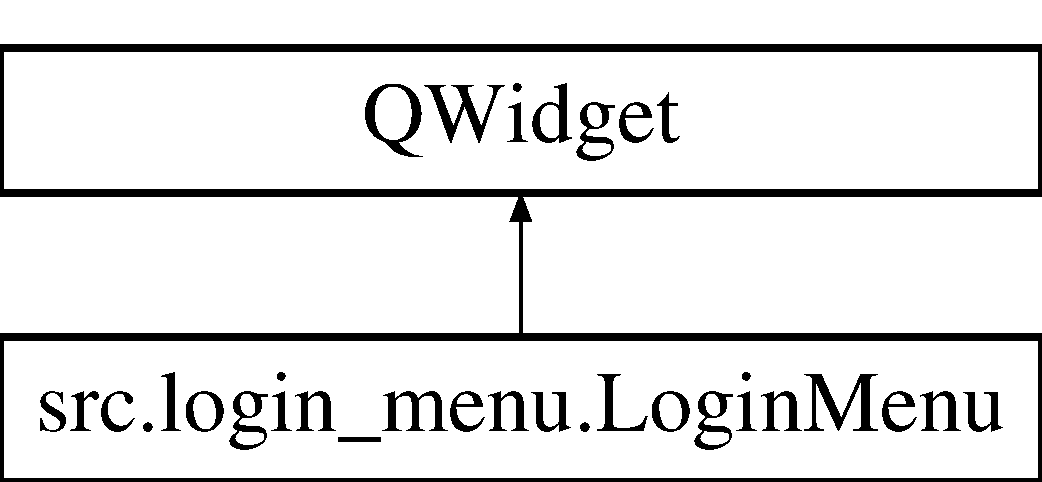
\includegraphics[height=2.000000cm]{classsrc_1_1login__menu_1_1_login_menu}
\end{center}
\end{figure}
\subsection*{Public Member Functions}
\begin{DoxyCompactItemize}
\item 
\hypertarget{classsrc_1_1login__menu_1_1_login_menu_a33638b382a7b9e5c95163bae3900d5b3}{}def {\bfseries \+\_\+\+\_\+init\+\_\+\+\_\+}\label{classsrc_1_1login__menu_1_1_login_menu_a33638b382a7b9e5c95163bae3900d5b3}

\item 
def \hyperlink{classsrc_1_1login__menu_1_1_login_menu_a5114077865bfc30e8adef2f90cd27d85}{init\+U\+I} (self)
\begin{DoxyCompactList}\small\item\em This method initialize the G\+U\+I of the login menu. \end{DoxyCompactList}\item 
def \hyperlink{classsrc_1_1login__menu_1_1_login_menu_a75303935e17e43388fd4ef3df029944e}{login} (self)
\begin{DoxyCompactList}\small\item\em this method is used to login an existing user. \end{DoxyCompactList}\item 
def \hyperlink{classsrc_1_1login__menu_1_1_login_menu_af6ee6a8dee90f1a94a506400356707ad}{register} (self)
\begin{DoxyCompactList}\small\item\em this method is used to register a new user. \end{DoxyCompactList}\end{DoxyCompactItemize}
\subsection*{Public Attributes}
\begin{DoxyCompactItemize}
\item 
\hyperlink{classsrc_1_1login__menu_1_1_login_menu_a9a3d5cb39385fb4b3d10f46af5543205}{db}
\begin{DoxyCompactList}\small\item\em instance of the database. \end{DoxyCompactList}\item 
\hyperlink{classsrc_1_1login__menu_1_1_login_menu_a07a65e6211f15b49d6e6abc0daac320b}{sign\+Up\+Title}
\begin{DoxyCompactList}\small\item\em is a Q\+Label to show the signup Title. \end{DoxyCompactList}\item 
\hyperlink{classsrc_1_1login__menu_1_1_login_menu_a6ba84d7d5a18940588ad710b7f6f964c}{your\+Name}
\begin{DoxyCompactList}\small\item\em is a Q\+Line\+Edit that creates a field the user uses to enter his name. \end{DoxyCompactList}\item 
\hyperlink{classsrc_1_1login__menu_1_1_login_menu_a6b5acd3b5dd7c538b601cf8ab1b1d4cf}{username}
\begin{DoxyCompactList}\small\item\em is a Q\+Line\+Edit that creates a field the user uses to enter his username. \end{DoxyCompactList}\item 
\hypertarget{classsrc_1_1login__menu_1_1_login_menu_a036845330836e34588c87e2d73f53b85}{}\hyperlink{classsrc_1_1login__menu_1_1_login_menu_a036845330836e34588c87e2d73f53b85}{password}\label{classsrc_1_1login__menu_1_1_login_menu_a036845330836e34588c87e2d73f53b85}

\begin{DoxyCompactList}\small\item\em is a Q\+Line\+Edit that creates a field the user uses to enter his password \end{DoxyCompactList}\item 
\hyperlink{classsrc_1_1login__menu_1_1_login_menu_a2d518012477c43a0d5b77385e2e4209f}{sign\+Up\+Button}
\begin{DoxyCompactList}\small\item\em is a button that calls the \hyperlink{classsrc_1_1login__menu_1_1_login_menu_af6ee6a8dee90f1a94a506400356707ad}{register()} method when clicked. \end{DoxyCompactList}\item 
\hyperlink{classsrc_1_1login__menu_1_1_login_menu_adce86324539cbf7d5a398d8afba6a439}{login\+Title}
\begin{DoxyCompactList}\small\item\em is a Q\+Label to show the login Title. \end{DoxyCompactList}\item 
\hyperlink{classsrc_1_1login__menu_1_1_login_menu_a762640516f0435f5764308fd0f00a6c9}{login\+Username}
\begin{DoxyCompactList}\small\item\em is a Q\+Line\+Edit that creates a field the user uses to enter his username. \end{DoxyCompactList}\item 
\hyperlink{classsrc_1_1login__menu_1_1_login_menu_a6c0c5ab8b48e62ccb26a472e6e7790c9}{login\+Password}
\begin{DoxyCompactList}\small\item\em is a Q\+Line\+Edit that creates a field the user uses to enter his password. \end{DoxyCompactList}\item 
\hyperlink{classsrc_1_1login__menu_1_1_login_menu_a6e91fe2dc9a5b4bb26019242e84ce986}{login\+Button}
\begin{DoxyCompactList}\small\item\em is a button that calls the \hyperlink{classsrc_1_1login__menu_1_1_login_menu_a75303935e17e43388fd4ef3df029944e}{login()} method when clicked. \end{DoxyCompactList}\end{DoxyCompactItemize}
\subsection*{Static Public Attributes}
\begin{DoxyCompactItemize}
\item 
tuple \hyperlink{classsrc_1_1login__menu_1_1_login_menu_a0c7d684b7c11fd92f8de9beee9cf2a9f}{login\+Success\+Signal} = Qt\+Core.\+pyqt\+Signal()
\begin{DoxyCompactList}\small\item\em Signal which will be used to launch the main menu. \end{DoxyCompactList}\item 
\hyperlink{classsrc_1_1login__menu_1_1_login_menu_a3c59b83a7a55f2334a015dfc722e86da}{logged\+Username} = None
\begin{DoxyCompactList}\small\item\em the currently logged in user\textquotesingle{}s username. \end{DoxyCompactList}\end{DoxyCompactItemize}


\subsection{Detailed Description}
This class is a widget that displays the login menu. 

It includes the following buttons and fields that the user can interact with\+:~\newline
you\+Name\+: is a Line\+Edit widget the user uses to enter his name.~\newline
username\+: is a Line\+Edit widget the user uses to enter his username at login or signup.~\newline
password\+: is a Line\+Edit widget the user uses to enter his password at login or signup.~\newline
signup\+Button\+: calls \hyperlink{classsrc_1_1login__menu_1_1_login_menu_af6ee6a8dee90f1a94a506400356707ad}{register()} method when clicked.~\newline
login\+Button\+: calls \hyperlink{classsrc_1_1login__menu_1_1_login_menu_a75303935e17e43388fd4ef3df029944e}{login()} method when clicked.~\newline
 

\subsection{Member Function Documentation}
\hypertarget{classsrc_1_1login__menu_1_1_login_menu_a5114077865bfc30e8adef2f90cd27d85}{}\index{src\+::login\+\_\+menu\+::\+Login\+Menu@{src\+::login\+\_\+menu\+::\+Login\+Menu}!init\+U\+I@{init\+U\+I}}
\index{init\+U\+I@{init\+U\+I}!src\+::login\+\_\+menu\+::\+Login\+Menu@{src\+::login\+\_\+menu\+::\+Login\+Menu}}
\subsubsection[{init\+U\+I}]{\setlength{\rightskip}{0pt plus 5cm}def src.\+login\+\_\+menu.\+Login\+Menu.\+init\+U\+I (
\begin{DoxyParamCaption}
\item[{}]{self}
\end{DoxyParamCaption}
)}\label{classsrc_1_1login__menu_1_1_login_menu_a5114077865bfc30e8adef2f90cd27d85}


This method initialize the G\+U\+I of the login menu. 

\hypertarget{classsrc_1_1login__menu_1_1_login_menu_a75303935e17e43388fd4ef3df029944e}{}\index{src\+::login\+\_\+menu\+::\+Login\+Menu@{src\+::login\+\_\+menu\+::\+Login\+Menu}!login@{login}}
\index{login@{login}!src\+::login\+\_\+menu\+::\+Login\+Menu@{src\+::login\+\_\+menu\+::\+Login\+Menu}}
\subsubsection[{login}]{\setlength{\rightskip}{0pt plus 5cm}def src.\+login\+\_\+menu.\+Login\+Menu.\+login (
\begin{DoxyParamCaption}
\item[{}]{self}
\end{DoxyParamCaption}
)}\label{classsrc_1_1login__menu_1_1_login_menu_a75303935e17e43388fd4ef3df029944e}


this method is used to login an existing user. 

it verifies if the user\textquotesingle{}s information match an existing user account and then emit login\+Success\+Signal. \hypertarget{classsrc_1_1login__menu_1_1_login_menu_af6ee6a8dee90f1a94a506400356707ad}{}\index{src\+::login\+\_\+menu\+::\+Login\+Menu@{src\+::login\+\_\+menu\+::\+Login\+Menu}!register@{register}}
\index{register@{register}!src\+::login\+\_\+menu\+::\+Login\+Menu@{src\+::login\+\_\+menu\+::\+Login\+Menu}}
\subsubsection[{register}]{\setlength{\rightskip}{0pt plus 5cm}def src.\+login\+\_\+menu.\+Login\+Menu.\+register (
\begin{DoxyParamCaption}
\item[{}]{self}
\end{DoxyParamCaption}
)}\label{classsrc_1_1login__menu_1_1_login_menu_af6ee6a8dee90f1a94a506400356707ad}


this method is used to register a new user. 

It first verifies if the user\textquotesingle{}s username and password follow the restrictions. 

\subsection{Member Data Documentation}
\hypertarget{classsrc_1_1login__menu_1_1_login_menu_a9a3d5cb39385fb4b3d10f46af5543205}{}\index{src\+::login\+\_\+menu\+::\+Login\+Menu@{src\+::login\+\_\+menu\+::\+Login\+Menu}!db@{db}}
\index{db@{db}!src\+::login\+\_\+menu\+::\+Login\+Menu@{src\+::login\+\_\+menu\+::\+Login\+Menu}}
\subsubsection[{db}]{\setlength{\rightskip}{0pt plus 5cm}src.\+login\+\_\+menu.\+Login\+Menu.\+db}\label{classsrc_1_1login__menu_1_1_login_menu_a9a3d5cb39385fb4b3d10f46af5543205}


instance of the database. 

\hypertarget{classsrc_1_1login__menu_1_1_login_menu_a3c59b83a7a55f2334a015dfc722e86da}{}\index{src\+::login\+\_\+menu\+::\+Login\+Menu@{src\+::login\+\_\+menu\+::\+Login\+Menu}!logged\+Username@{logged\+Username}}
\index{logged\+Username@{logged\+Username}!src\+::login\+\_\+menu\+::\+Login\+Menu@{src\+::login\+\_\+menu\+::\+Login\+Menu}}
\subsubsection[{logged\+Username}]{\setlength{\rightskip}{0pt plus 5cm}src.\+login\+\_\+menu.\+Login\+Menu.\+logged\+Username = None\hspace{0.3cm}{\ttfamily [static]}}\label{classsrc_1_1login__menu_1_1_login_menu_a3c59b83a7a55f2334a015dfc722e86da}


the currently logged in user\textquotesingle{}s username. 

initialized to \textquotesingle{}None\textquotesingle{} if not currently logged in. \hypertarget{classsrc_1_1login__menu_1_1_login_menu_a6e91fe2dc9a5b4bb26019242e84ce986}{}\index{src\+::login\+\_\+menu\+::\+Login\+Menu@{src\+::login\+\_\+menu\+::\+Login\+Menu}!login\+Button@{login\+Button}}
\index{login\+Button@{login\+Button}!src\+::login\+\_\+menu\+::\+Login\+Menu@{src\+::login\+\_\+menu\+::\+Login\+Menu}}
\subsubsection[{login\+Button}]{\setlength{\rightskip}{0pt plus 5cm}src.\+login\+\_\+menu.\+Login\+Menu.\+login\+Button}\label{classsrc_1_1login__menu_1_1_login_menu_a6e91fe2dc9a5b4bb26019242e84ce986}


is a button that calls the \hyperlink{classsrc_1_1login__menu_1_1_login_menu_a75303935e17e43388fd4ef3df029944e}{login()} method when clicked. 

\hypertarget{classsrc_1_1login__menu_1_1_login_menu_a6c0c5ab8b48e62ccb26a472e6e7790c9}{}\index{src\+::login\+\_\+menu\+::\+Login\+Menu@{src\+::login\+\_\+menu\+::\+Login\+Menu}!login\+Password@{login\+Password}}
\index{login\+Password@{login\+Password}!src\+::login\+\_\+menu\+::\+Login\+Menu@{src\+::login\+\_\+menu\+::\+Login\+Menu}}
\subsubsection[{login\+Password}]{\setlength{\rightskip}{0pt plus 5cm}src.\+login\+\_\+menu.\+Login\+Menu.\+login\+Password}\label{classsrc_1_1login__menu_1_1_login_menu_a6c0c5ab8b48e62ccb26a472e6e7790c9}


is a Q\+Line\+Edit that creates a field the user uses to enter his password. 

\hypertarget{classsrc_1_1login__menu_1_1_login_menu_a0c7d684b7c11fd92f8de9beee9cf2a9f}{}\index{src\+::login\+\_\+menu\+::\+Login\+Menu@{src\+::login\+\_\+menu\+::\+Login\+Menu}!login\+Success\+Signal@{login\+Success\+Signal}}
\index{login\+Success\+Signal@{login\+Success\+Signal}!src\+::login\+\_\+menu\+::\+Login\+Menu@{src\+::login\+\_\+menu\+::\+Login\+Menu}}
\subsubsection[{login\+Success\+Signal}]{\setlength{\rightskip}{0pt plus 5cm}tuple src.\+login\+\_\+menu.\+Login\+Menu.\+login\+Success\+Signal = Qt\+Core.\+pyqt\+Signal()\hspace{0.3cm}{\ttfamily [static]}}\label{classsrc_1_1login__menu_1_1_login_menu_a0c7d684b7c11fd92f8de9beee9cf2a9f}


Signal which will be used to launch the main menu. 

\hypertarget{classsrc_1_1login__menu_1_1_login_menu_adce86324539cbf7d5a398d8afba6a439}{}\index{src\+::login\+\_\+menu\+::\+Login\+Menu@{src\+::login\+\_\+menu\+::\+Login\+Menu}!login\+Title@{login\+Title}}
\index{login\+Title@{login\+Title}!src\+::login\+\_\+menu\+::\+Login\+Menu@{src\+::login\+\_\+menu\+::\+Login\+Menu}}
\subsubsection[{login\+Title}]{\setlength{\rightskip}{0pt plus 5cm}src.\+login\+\_\+menu.\+Login\+Menu.\+login\+Title}\label{classsrc_1_1login__menu_1_1_login_menu_adce86324539cbf7d5a398d8afba6a439}


is a Q\+Label to show the login Title. 

\hypertarget{classsrc_1_1login__menu_1_1_login_menu_a762640516f0435f5764308fd0f00a6c9}{}\index{src\+::login\+\_\+menu\+::\+Login\+Menu@{src\+::login\+\_\+menu\+::\+Login\+Menu}!login\+Username@{login\+Username}}
\index{login\+Username@{login\+Username}!src\+::login\+\_\+menu\+::\+Login\+Menu@{src\+::login\+\_\+menu\+::\+Login\+Menu}}
\subsubsection[{login\+Username}]{\setlength{\rightskip}{0pt plus 5cm}src.\+login\+\_\+menu.\+Login\+Menu.\+login\+Username}\label{classsrc_1_1login__menu_1_1_login_menu_a762640516f0435f5764308fd0f00a6c9}


is a Q\+Line\+Edit that creates a field the user uses to enter his username. 

\hypertarget{classsrc_1_1login__menu_1_1_login_menu_a2d518012477c43a0d5b77385e2e4209f}{}\index{src\+::login\+\_\+menu\+::\+Login\+Menu@{src\+::login\+\_\+menu\+::\+Login\+Menu}!sign\+Up\+Button@{sign\+Up\+Button}}
\index{sign\+Up\+Button@{sign\+Up\+Button}!src\+::login\+\_\+menu\+::\+Login\+Menu@{src\+::login\+\_\+menu\+::\+Login\+Menu}}
\subsubsection[{sign\+Up\+Button}]{\setlength{\rightskip}{0pt plus 5cm}src.\+login\+\_\+menu.\+Login\+Menu.\+sign\+Up\+Button}\label{classsrc_1_1login__menu_1_1_login_menu_a2d518012477c43a0d5b77385e2e4209f}


is a button that calls the \hyperlink{classsrc_1_1login__menu_1_1_login_menu_af6ee6a8dee90f1a94a506400356707ad}{register()} method when clicked. 

\hypertarget{classsrc_1_1login__menu_1_1_login_menu_a07a65e6211f15b49d6e6abc0daac320b}{}\index{src\+::login\+\_\+menu\+::\+Login\+Menu@{src\+::login\+\_\+menu\+::\+Login\+Menu}!sign\+Up\+Title@{sign\+Up\+Title}}
\index{sign\+Up\+Title@{sign\+Up\+Title}!src\+::login\+\_\+menu\+::\+Login\+Menu@{src\+::login\+\_\+menu\+::\+Login\+Menu}}
\subsubsection[{sign\+Up\+Title}]{\setlength{\rightskip}{0pt plus 5cm}src.\+login\+\_\+menu.\+Login\+Menu.\+sign\+Up\+Title}\label{classsrc_1_1login__menu_1_1_login_menu_a07a65e6211f15b49d6e6abc0daac320b}


is a Q\+Label to show the signup Title. 

\hypertarget{classsrc_1_1login__menu_1_1_login_menu_a6b5acd3b5dd7c538b601cf8ab1b1d4cf}{}\index{src\+::login\+\_\+menu\+::\+Login\+Menu@{src\+::login\+\_\+menu\+::\+Login\+Menu}!username@{username}}
\index{username@{username}!src\+::login\+\_\+menu\+::\+Login\+Menu@{src\+::login\+\_\+menu\+::\+Login\+Menu}}
\subsubsection[{username}]{\setlength{\rightskip}{0pt plus 5cm}src.\+login\+\_\+menu.\+Login\+Menu.\+username}\label{classsrc_1_1login__menu_1_1_login_menu_a6b5acd3b5dd7c538b601cf8ab1b1d4cf}


is a Q\+Line\+Edit that creates a field the user uses to enter his username. 

\hypertarget{classsrc_1_1login__menu_1_1_login_menu_a6ba84d7d5a18940588ad710b7f6f964c}{}\index{src\+::login\+\_\+menu\+::\+Login\+Menu@{src\+::login\+\_\+menu\+::\+Login\+Menu}!your\+Name@{your\+Name}}
\index{your\+Name@{your\+Name}!src\+::login\+\_\+menu\+::\+Login\+Menu@{src\+::login\+\_\+menu\+::\+Login\+Menu}}
\subsubsection[{your\+Name}]{\setlength{\rightskip}{0pt plus 5cm}src.\+login\+\_\+menu.\+Login\+Menu.\+your\+Name}\label{classsrc_1_1login__menu_1_1_login_menu_a6ba84d7d5a18940588ad710b7f6f964c}


is a Q\+Line\+Edit that creates a field the user uses to enter his name. 



The documentation for this class was generated from the following file\+:\begin{DoxyCompactItemize}
\item 
src/login\+\_\+menu.\+py\end{DoxyCompactItemize}

\hypertarget{classsrc_1_1main__menu_1_1_main_menu}{}\section{src.\+main\+\_\+menu.\+Main\+Menu Class Reference}
\label{classsrc_1_1main__menu_1_1_main_menu}\index{src.\+main\+\_\+menu.\+Main\+Menu@{src.\+main\+\_\+menu.\+Main\+Menu}}
Inheritance diagram for src.\+main\+\_\+menu.\+Main\+Menu\+:\begin{figure}[H]
\begin{center}
\leavevmode
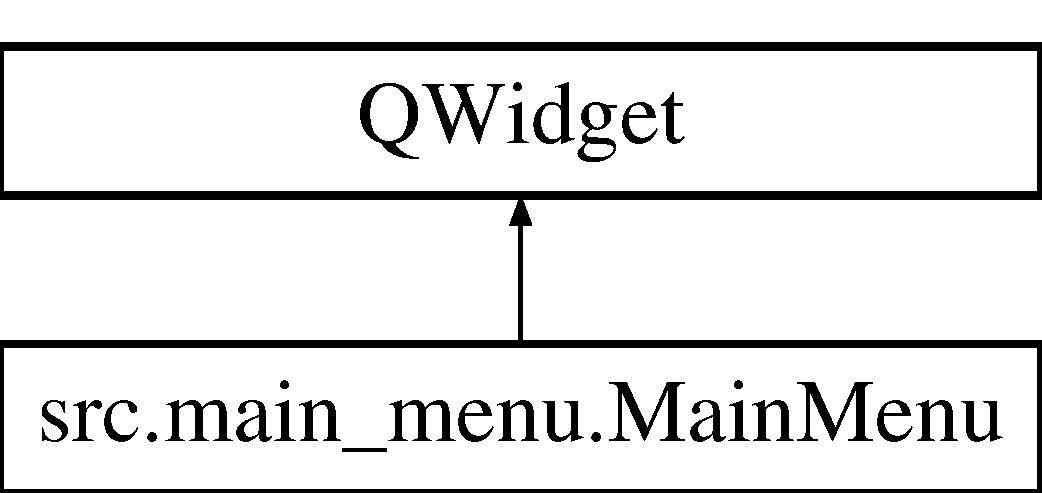
\includegraphics[height=2.000000cm]{classsrc_1_1main__menu_1_1_main_menu}
\end{center}
\end{figure}
\subsection*{Public Member Functions}
\begin{DoxyCompactItemize}
\item 
\hypertarget{classsrc_1_1main__menu_1_1_main_menu_a138987af797121617841ccb0cdd20121}{}def {\bfseries \+\_\+\+\_\+init\+\_\+\+\_\+}\label{classsrc_1_1main__menu_1_1_main_menu_a138987af797121617841ccb0cdd20121}

\item 
def \hyperlink{classsrc_1_1main__menu_1_1_main_menu_abe71c56b747e1f76a2b73b542875a4d7}{init\+U\+I} (self)
\begin{DoxyCompactList}\small\item\em This method initialize the G\+U\+I of Main menu. \end{DoxyCompactList}\item 
def \hyperlink{classsrc_1_1main__menu_1_1_main_menu_adaa5ceb3caccddfacf97ca9befd21ae5}{play} (self)
\begin{DoxyCompactList}\small\item\em emit play\+Game\+Signal when called. \end{DoxyCompactList}\item 
def \hyperlink{classsrc_1_1main__menu_1_1_main_menu_ac60fcc9e2384edbf984c094682c61624}{logout} (self)
\begin{DoxyCompactList}\small\item\em emit logout\+Game\+Signal when called. \end{DoxyCompactList}\item 
def \hyperlink{classsrc_1_1main__menu_1_1_main_menu_ab2872e528109b4747bc169235302d3ae}{quit} (self)
\begin{DoxyCompactList}\small\item\em emit quit\+Game\+Signal when called. \end{DoxyCompactList}\item 
def \hyperlink{classsrc_1_1main__menu_1_1_main_menu_ad92f678a32751ee9d592fd64d487126b}{show\+Leaderboard} (self)
\begin{DoxyCompactList}\small\item\em emit show\+Leaderboard\+Signal when called. \end{DoxyCompactList}\item 
\hypertarget{classsrc_1_1main__menu_1_1_main_menu_a9f5509f22d8daa7510daa6bb592e5f73}{}def \hyperlink{classsrc_1_1main__menu_1_1_main_menu_a9f5509f22d8daa7510daa6bb592e5f73}{show\+Account\+Settings\+Menu} (self)\label{classsrc_1_1main__menu_1_1_main_menu_a9f5509f22d8daa7510daa6bb592e5f73}

\begin{DoxyCompactList}\small\item\em emit change\+Settings\+Signal when called \end{DoxyCompactList}\item 
def \hyperlink{classsrc_1_1main__menu_1_1_main_menu_a5a8bd4179063fdebe0f679b4501e6642}{load} (self)
\begin{DoxyCompactList}\small\item\em emit load\+Menu\+Signal when called. \end{DoxyCompactList}\end{DoxyCompactItemize}
\subsection*{Static Public Attributes}
\begin{DoxyCompactItemize}
\item 
tuple \hyperlink{classsrc_1_1main__menu_1_1_main_menu_a5649447e46d6bd6bdc5f1289941c8c02}{play\+Game\+Signal} = Qt\+Core.\+pyqt\+Signal()
\begin{DoxyCompactList}\small\item\em Signal which will be used to launch the game. \end{DoxyCompactList}\item 
tuple \hyperlink{classsrc_1_1main__menu_1_1_main_menu_ac8a9bae484f207fa58edd090112c8be3}{logout\+Game\+Signal} = Qt\+Core.\+pyqt\+Signal()
\begin{DoxyCompactList}\small\item\em Signal which will be used to exit the current user and send it back to login menu. \end{DoxyCompactList}\item 
tuple \hyperlink{classsrc_1_1main__menu_1_1_main_menu_adb966ecda1f332af67efc3c3b3adf8bd}{quit\+Game\+Signal} = Qt\+Core.\+pyqt\+Signal()
\begin{DoxyCompactList}\small\item\em Signal which will be used to quit the whole application. \end{DoxyCompactList}\item 
tuple \hyperlink{classsrc_1_1main__menu_1_1_main_menu_aa737b525a5e965eb6af321d25baa787c}{show\+Leaderboard\+Signal} = Qt\+Core.\+pyqt\+Signal(int)
\begin{DoxyCompactList}\small\item\em Signal which will be used to to launch the leaderboard. \end{DoxyCompactList}\item 
tuple \hyperlink{classsrc_1_1main__menu_1_1_main_menu_a51466fb736e3368249412c501aa18741}{load\+Menu\+Signal} = Qt\+Core.\+pyqt\+Signal(int)
\begin{DoxyCompactList}\small\item\em Signal which will launch the load menu. \end{DoxyCompactList}\item 
tuple \hyperlink{classsrc_1_1main__menu_1_1_main_menu_a7a76ee92b8b02099e74f0d5ad107ff34}{change\+Settings\+Signal} = Qt\+Core.\+pyqt\+Signal()
\begin{DoxyCompactList}\small\item\em Signal which will launch the account settings menu. \end{DoxyCompactList}\end{DoxyCompactItemize}


\subsection{Member Function Documentation}
\hypertarget{classsrc_1_1main__menu_1_1_main_menu_abe71c56b747e1f76a2b73b542875a4d7}{}\index{src\+::main\+\_\+menu\+::\+Main\+Menu@{src\+::main\+\_\+menu\+::\+Main\+Menu}!init\+U\+I@{init\+U\+I}}
\index{init\+U\+I@{init\+U\+I}!src\+::main\+\_\+menu\+::\+Main\+Menu@{src\+::main\+\_\+menu\+::\+Main\+Menu}}
\subsubsection[{init\+U\+I}]{\setlength{\rightskip}{0pt plus 5cm}def src.\+main\+\_\+menu.\+Main\+Menu.\+init\+U\+I (
\begin{DoxyParamCaption}
\item[{}]{self}
\end{DoxyParamCaption}
)}\label{classsrc_1_1main__menu_1_1_main_menu_abe71c56b747e1f76a2b73b542875a4d7}


This method initialize the G\+U\+I of Main menu. 

\hypertarget{classsrc_1_1main__menu_1_1_main_menu_a5a8bd4179063fdebe0f679b4501e6642}{}\index{src\+::main\+\_\+menu\+::\+Main\+Menu@{src\+::main\+\_\+menu\+::\+Main\+Menu}!load@{load}}
\index{load@{load}!src\+::main\+\_\+menu\+::\+Main\+Menu@{src\+::main\+\_\+menu\+::\+Main\+Menu}}
\subsubsection[{load}]{\setlength{\rightskip}{0pt plus 5cm}def src.\+main\+\_\+menu.\+Main\+Menu.\+load (
\begin{DoxyParamCaption}
\item[{}]{self}
\end{DoxyParamCaption}
)}\label{classsrc_1_1main__menu_1_1_main_menu_a5a8bd4179063fdebe0f679b4501e6642}


emit load\+Menu\+Signal when called. 

\hypertarget{classsrc_1_1main__menu_1_1_main_menu_ac60fcc9e2384edbf984c094682c61624}{}\index{src\+::main\+\_\+menu\+::\+Main\+Menu@{src\+::main\+\_\+menu\+::\+Main\+Menu}!logout@{logout}}
\index{logout@{logout}!src\+::main\+\_\+menu\+::\+Main\+Menu@{src\+::main\+\_\+menu\+::\+Main\+Menu}}
\subsubsection[{logout}]{\setlength{\rightskip}{0pt plus 5cm}def src.\+main\+\_\+menu.\+Main\+Menu.\+logout (
\begin{DoxyParamCaption}
\item[{}]{self}
\end{DoxyParamCaption}
)}\label{classsrc_1_1main__menu_1_1_main_menu_ac60fcc9e2384edbf984c094682c61624}


emit logout\+Game\+Signal when called. 

\hypertarget{classsrc_1_1main__menu_1_1_main_menu_adaa5ceb3caccddfacf97ca9befd21ae5}{}\index{src\+::main\+\_\+menu\+::\+Main\+Menu@{src\+::main\+\_\+menu\+::\+Main\+Menu}!play@{play}}
\index{play@{play}!src\+::main\+\_\+menu\+::\+Main\+Menu@{src\+::main\+\_\+menu\+::\+Main\+Menu}}
\subsubsection[{play}]{\setlength{\rightskip}{0pt plus 5cm}def src.\+main\+\_\+menu.\+Main\+Menu.\+play (
\begin{DoxyParamCaption}
\item[{}]{self}
\end{DoxyParamCaption}
)}\label{classsrc_1_1main__menu_1_1_main_menu_adaa5ceb3caccddfacf97ca9befd21ae5}


emit play\+Game\+Signal when called. 

\hypertarget{classsrc_1_1main__menu_1_1_main_menu_ab2872e528109b4747bc169235302d3ae}{}\index{src\+::main\+\_\+menu\+::\+Main\+Menu@{src\+::main\+\_\+menu\+::\+Main\+Menu}!quit@{quit}}
\index{quit@{quit}!src\+::main\+\_\+menu\+::\+Main\+Menu@{src\+::main\+\_\+menu\+::\+Main\+Menu}}
\subsubsection[{quit}]{\setlength{\rightskip}{0pt plus 5cm}def src.\+main\+\_\+menu.\+Main\+Menu.\+quit (
\begin{DoxyParamCaption}
\item[{}]{self}
\end{DoxyParamCaption}
)}\label{classsrc_1_1main__menu_1_1_main_menu_ab2872e528109b4747bc169235302d3ae}


emit quit\+Game\+Signal when called. 

\hypertarget{classsrc_1_1main__menu_1_1_main_menu_ad92f678a32751ee9d592fd64d487126b}{}\index{src\+::main\+\_\+menu\+::\+Main\+Menu@{src\+::main\+\_\+menu\+::\+Main\+Menu}!show\+Leaderboard@{show\+Leaderboard}}
\index{show\+Leaderboard@{show\+Leaderboard}!src\+::main\+\_\+menu\+::\+Main\+Menu@{src\+::main\+\_\+menu\+::\+Main\+Menu}}
\subsubsection[{show\+Leaderboard}]{\setlength{\rightskip}{0pt plus 5cm}def src.\+main\+\_\+menu.\+Main\+Menu.\+show\+Leaderboard (
\begin{DoxyParamCaption}
\item[{}]{self}
\end{DoxyParamCaption}
)}\label{classsrc_1_1main__menu_1_1_main_menu_ad92f678a32751ee9d592fd64d487126b}


emit show\+Leaderboard\+Signal when called. 



\subsection{Member Data Documentation}
\hypertarget{classsrc_1_1main__menu_1_1_main_menu_a7a76ee92b8b02099e74f0d5ad107ff34}{}\index{src\+::main\+\_\+menu\+::\+Main\+Menu@{src\+::main\+\_\+menu\+::\+Main\+Menu}!change\+Settings\+Signal@{change\+Settings\+Signal}}
\index{change\+Settings\+Signal@{change\+Settings\+Signal}!src\+::main\+\_\+menu\+::\+Main\+Menu@{src\+::main\+\_\+menu\+::\+Main\+Menu}}
\subsubsection[{change\+Settings\+Signal}]{\setlength{\rightskip}{0pt plus 5cm}tuple src.\+main\+\_\+menu.\+Main\+Menu.\+change\+Settings\+Signal = Qt\+Core.\+pyqt\+Signal()\hspace{0.3cm}{\ttfamily [static]}}\label{classsrc_1_1main__menu_1_1_main_menu_a7a76ee92b8b02099e74f0d5ad107ff34}


Signal which will launch the account settings menu. 

\hypertarget{classsrc_1_1main__menu_1_1_main_menu_a51466fb736e3368249412c501aa18741}{}\index{src\+::main\+\_\+menu\+::\+Main\+Menu@{src\+::main\+\_\+menu\+::\+Main\+Menu}!load\+Menu\+Signal@{load\+Menu\+Signal}}
\index{load\+Menu\+Signal@{load\+Menu\+Signal}!src\+::main\+\_\+menu\+::\+Main\+Menu@{src\+::main\+\_\+menu\+::\+Main\+Menu}}
\subsubsection[{load\+Menu\+Signal}]{\setlength{\rightskip}{0pt plus 5cm}tuple src.\+main\+\_\+menu.\+Main\+Menu.\+load\+Menu\+Signal = Qt\+Core.\+pyqt\+Signal(int)\hspace{0.3cm}{\ttfamily [static]}}\label{classsrc_1_1main__menu_1_1_main_menu_a51466fb736e3368249412c501aa18741}


Signal which will launch the load menu. 

Also emit the int \textquotesingle{}previous\+Menu\textquotesingle{} to keep track of the menu it was called from. \hypertarget{classsrc_1_1main__menu_1_1_main_menu_ac8a9bae484f207fa58edd090112c8be3}{}\index{src\+::main\+\_\+menu\+::\+Main\+Menu@{src\+::main\+\_\+menu\+::\+Main\+Menu}!logout\+Game\+Signal@{logout\+Game\+Signal}}
\index{logout\+Game\+Signal@{logout\+Game\+Signal}!src\+::main\+\_\+menu\+::\+Main\+Menu@{src\+::main\+\_\+menu\+::\+Main\+Menu}}
\subsubsection[{logout\+Game\+Signal}]{\setlength{\rightskip}{0pt plus 5cm}tuple src.\+main\+\_\+menu.\+Main\+Menu.\+logout\+Game\+Signal = Qt\+Core.\+pyqt\+Signal()\hspace{0.3cm}{\ttfamily [static]}}\label{classsrc_1_1main__menu_1_1_main_menu_ac8a9bae484f207fa58edd090112c8be3}


Signal which will be used to exit the current user and send it back to login menu. 

\hypertarget{classsrc_1_1main__menu_1_1_main_menu_a5649447e46d6bd6bdc5f1289941c8c02}{}\index{src\+::main\+\_\+menu\+::\+Main\+Menu@{src\+::main\+\_\+menu\+::\+Main\+Menu}!play\+Game\+Signal@{play\+Game\+Signal}}
\index{play\+Game\+Signal@{play\+Game\+Signal}!src\+::main\+\_\+menu\+::\+Main\+Menu@{src\+::main\+\_\+menu\+::\+Main\+Menu}}
\subsubsection[{play\+Game\+Signal}]{\setlength{\rightskip}{0pt plus 5cm}tuple src.\+main\+\_\+menu.\+Main\+Menu.\+play\+Game\+Signal = Qt\+Core.\+pyqt\+Signal()\hspace{0.3cm}{\ttfamily [static]}}\label{classsrc_1_1main__menu_1_1_main_menu_a5649447e46d6bd6bdc5f1289941c8c02}


Signal which will be used to launch the game. 

\hypertarget{classsrc_1_1main__menu_1_1_main_menu_adb966ecda1f332af67efc3c3b3adf8bd}{}\index{src\+::main\+\_\+menu\+::\+Main\+Menu@{src\+::main\+\_\+menu\+::\+Main\+Menu}!quit\+Game\+Signal@{quit\+Game\+Signal}}
\index{quit\+Game\+Signal@{quit\+Game\+Signal}!src\+::main\+\_\+menu\+::\+Main\+Menu@{src\+::main\+\_\+menu\+::\+Main\+Menu}}
\subsubsection[{quit\+Game\+Signal}]{\setlength{\rightskip}{0pt plus 5cm}tuple src.\+main\+\_\+menu.\+Main\+Menu.\+quit\+Game\+Signal = Qt\+Core.\+pyqt\+Signal()\hspace{0.3cm}{\ttfamily [static]}}\label{classsrc_1_1main__menu_1_1_main_menu_adb966ecda1f332af67efc3c3b3adf8bd}


Signal which will be used to quit the whole application. 

\hypertarget{classsrc_1_1main__menu_1_1_main_menu_aa737b525a5e965eb6af321d25baa787c}{}\index{src\+::main\+\_\+menu\+::\+Main\+Menu@{src\+::main\+\_\+menu\+::\+Main\+Menu}!show\+Leaderboard\+Signal@{show\+Leaderboard\+Signal}}
\index{show\+Leaderboard\+Signal@{show\+Leaderboard\+Signal}!src\+::main\+\_\+menu\+::\+Main\+Menu@{src\+::main\+\_\+menu\+::\+Main\+Menu}}
\subsubsection[{show\+Leaderboard\+Signal}]{\setlength{\rightskip}{0pt plus 5cm}tuple src.\+main\+\_\+menu.\+Main\+Menu.\+show\+Leaderboard\+Signal = Qt\+Core.\+pyqt\+Signal(int)\hspace{0.3cm}{\ttfamily [static]}}\label{classsrc_1_1main__menu_1_1_main_menu_aa737b525a5e965eb6af321d25baa787c}


Signal which will be used to to launch the leaderboard. 

Also emit the int \textquotesingle{}previous\+Menu\textquotesingle{} to keep track of the menu it was called from. 

The documentation for this class was generated from the following file\+:\begin{DoxyCompactItemize}
\item 
src/main\+\_\+menu.\+py\end{DoxyCompactItemize}

\hypertarget{classsrc_1_1pause__menu_1_1_pause_menu}{}\section{src.\+pause\+\_\+menu.\+Pause\+Menu Class Reference}
\label{classsrc_1_1pause__menu_1_1_pause_menu}\index{src.\+pause\+\_\+menu.\+Pause\+Menu@{src.\+pause\+\_\+menu.\+Pause\+Menu}}
Inheritance diagram for src.\+pause\+\_\+menu.\+Pause\+Menu\+:\begin{figure}[H]
\begin{center}
\leavevmode
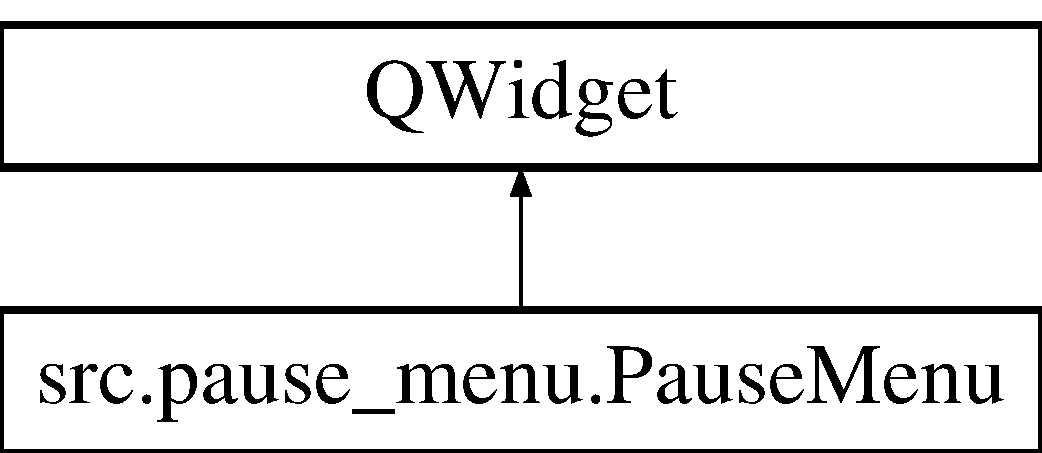
\includegraphics[height=2.000000cm]{classsrc_1_1pause__menu_1_1_pause_menu}
\end{center}
\end{figure}
\subsection*{Public Member Functions}
\begin{DoxyCompactItemize}
\item 
\hypertarget{classsrc_1_1pause__menu_1_1_pause_menu_a50b6571cbb54b07250cf74db412231dd}{}def {\bfseries \+\_\+\+\_\+init\+\_\+\+\_\+}\label{classsrc_1_1pause__menu_1_1_pause_menu_a50b6571cbb54b07250cf74db412231dd}

\item 
def \hyperlink{classsrc_1_1pause__menu_1_1_pause_menu_a9a5e36aa2482be916deefce1f4f23fcb}{init\+U\+I} (self)
\begin{DoxyCompactList}\small\item\em this method initialize the G\+U\+I of the pause menu. \end{DoxyCompactList}\item 
def \hyperlink{classsrc_1_1pause__menu_1_1_pause_menu_aaf160aa602ebd4ec91e9bc32d6d730f9}{resume} (self)
\begin{DoxyCompactList}\small\item\em emit resume\+Game\+Signal when called. \end{DoxyCompactList}\item 
def \hyperlink{classsrc_1_1pause__menu_1_1_pause_menu_a9f29e275aa812da5fad8730a41746677}{quit} (self)
\begin{DoxyCompactList}\small\item\em emit quit\+Game\+Signal when called. \end{DoxyCompactList}\item 
def \hyperlink{classsrc_1_1pause__menu_1_1_pause_menu_a9e3d8c0c94fdf4af682d6988f123888f}{show\+Leaderboard} (self)
\begin{DoxyCompactList}\small\item\em emit show\+Leaderboard\+Signal with parameter \textquotesingle{}constant.\+P\+A\+U\+S\+E\+\_\+\+M\+E\+N\+U\textquotesingle{} when called. \end{DoxyCompactList}\item 
def \hyperlink{classsrc_1_1pause__menu_1_1_pause_menu_affa6df962a7284b81fa60171119585b1}{back} (self)
\begin{DoxyCompactList}\small\item\em emit back\+To\+Main\+Menu\+Signal when called. \end{DoxyCompactList}\item 
def \hyperlink{classsrc_1_1pause__menu_1_1_pause_menu_a6950e08a6f9a87c87e9b77d606117eef}{save} (self)
\begin{DoxyCompactList}\small\item\em emit save\+Menu\+Signal when called. \end{DoxyCompactList}\item 
def \hyperlink{classsrc_1_1pause__menu_1_1_pause_menu_aa3714c919e9514631cd66c6714c1e243}{load} (self)
\begin{DoxyCompactList}\small\item\em emit load\+Menu\+Signal with parameter \textquotesingle{}constant.\+P\+A\+U\+S\+E\+\_\+\+M\+E\+N\+U\textquotesingle{} when called. \end{DoxyCompactList}\end{DoxyCompactItemize}
\subsection*{Static Public Attributes}
\begin{DoxyCompactItemize}
\item 
tuple \hyperlink{classsrc_1_1pause__menu_1_1_pause_menu_a0b97feb3939cd6be81c71ba6dbe67669}{resume\+Game\+Signal} = Qt\+Core.\+pyqt\+Signal()
\begin{DoxyCompactList}\small\item\em Signal which will be used to resume the current game. \end{DoxyCompactList}\item 
tuple \hyperlink{classsrc_1_1pause__menu_1_1_pause_menu_aea554e6749ca45f516618711530a1acd}{quit\+Game\+Signal} = Qt\+Core.\+pyqt\+Signal()
\begin{DoxyCompactList}\small\item\em Signal which will be used to quit the whole application. \end{DoxyCompactList}\item 
tuple \hyperlink{classsrc_1_1pause__menu_1_1_pause_menu_abaa0c6d5831d9bfb1d99d7431e47a981}{show\+Leaderboard\+Signal} = Qt\+Core.\+pyqt\+Signal(int)
\begin{DoxyCompactList}\small\item\em Signal which will be used to launch the leaderboard. \end{DoxyCompactList}\item 
tuple \hyperlink{classsrc_1_1pause__menu_1_1_pause_menu_a48613202c1a9051758755bf8fcdd2ecc}{save\+Menu\+Signal} = Qt\+Core.\+pyqt\+Signal()
\begin{DoxyCompactList}\small\item\em Signal which will be used to launch save menu. \end{DoxyCompactList}\item 
tuple \hyperlink{classsrc_1_1pause__menu_1_1_pause_menu_ae1851c6cab071ed1a4473320110432d8}{load\+Menu\+Signal} = Qt\+Core.\+pyqt\+Signal(int)
\begin{DoxyCompactList}\small\item\em Signal which will be used to launch load menu. \end{DoxyCompactList}\item 
tuple \hyperlink{classsrc_1_1pause__menu_1_1_pause_menu_adc8bc5514ba8991d100512319659d24e}{back\+To\+Main\+Menu\+Signal} = Qt\+Core.\+pyqt\+Signal()
\begin{DoxyCompactList}\small\item\em Signal which will be used to go back to the main menu. \end{DoxyCompactList}\end{DoxyCompactItemize}


\subsection{Member Function Documentation}
\hypertarget{classsrc_1_1pause__menu_1_1_pause_menu_affa6df962a7284b81fa60171119585b1}{}\index{src\+::pause\+\_\+menu\+::\+Pause\+Menu@{src\+::pause\+\_\+menu\+::\+Pause\+Menu}!back@{back}}
\index{back@{back}!src\+::pause\+\_\+menu\+::\+Pause\+Menu@{src\+::pause\+\_\+menu\+::\+Pause\+Menu}}
\subsubsection[{back}]{\setlength{\rightskip}{0pt plus 5cm}def src.\+pause\+\_\+menu.\+Pause\+Menu.\+back (
\begin{DoxyParamCaption}
\item[{}]{self}
\end{DoxyParamCaption}
)}\label{classsrc_1_1pause__menu_1_1_pause_menu_affa6df962a7284b81fa60171119585b1}


emit back\+To\+Main\+Menu\+Signal when called. 

\hypertarget{classsrc_1_1pause__menu_1_1_pause_menu_a9a5e36aa2482be916deefce1f4f23fcb}{}\index{src\+::pause\+\_\+menu\+::\+Pause\+Menu@{src\+::pause\+\_\+menu\+::\+Pause\+Menu}!init\+U\+I@{init\+U\+I}}
\index{init\+U\+I@{init\+U\+I}!src\+::pause\+\_\+menu\+::\+Pause\+Menu@{src\+::pause\+\_\+menu\+::\+Pause\+Menu}}
\subsubsection[{init\+U\+I}]{\setlength{\rightskip}{0pt plus 5cm}def src.\+pause\+\_\+menu.\+Pause\+Menu.\+init\+U\+I (
\begin{DoxyParamCaption}
\item[{}]{self}
\end{DoxyParamCaption}
)}\label{classsrc_1_1pause__menu_1_1_pause_menu_a9a5e36aa2482be916deefce1f4f23fcb}


this method initialize the G\+U\+I of the pause menu. 

\hypertarget{classsrc_1_1pause__menu_1_1_pause_menu_aa3714c919e9514631cd66c6714c1e243}{}\index{src\+::pause\+\_\+menu\+::\+Pause\+Menu@{src\+::pause\+\_\+menu\+::\+Pause\+Menu}!load@{load}}
\index{load@{load}!src\+::pause\+\_\+menu\+::\+Pause\+Menu@{src\+::pause\+\_\+menu\+::\+Pause\+Menu}}
\subsubsection[{load}]{\setlength{\rightskip}{0pt plus 5cm}def src.\+pause\+\_\+menu.\+Pause\+Menu.\+load (
\begin{DoxyParamCaption}
\item[{}]{self}
\end{DoxyParamCaption}
)}\label{classsrc_1_1pause__menu_1_1_pause_menu_aa3714c919e9514631cd66c6714c1e243}


emit load\+Menu\+Signal with parameter \textquotesingle{}constant.\+P\+A\+U\+S\+E\+\_\+\+M\+E\+N\+U\textquotesingle{} when called. 

\hypertarget{classsrc_1_1pause__menu_1_1_pause_menu_a9f29e275aa812da5fad8730a41746677}{}\index{src\+::pause\+\_\+menu\+::\+Pause\+Menu@{src\+::pause\+\_\+menu\+::\+Pause\+Menu}!quit@{quit}}
\index{quit@{quit}!src\+::pause\+\_\+menu\+::\+Pause\+Menu@{src\+::pause\+\_\+menu\+::\+Pause\+Menu}}
\subsubsection[{quit}]{\setlength{\rightskip}{0pt plus 5cm}def src.\+pause\+\_\+menu.\+Pause\+Menu.\+quit (
\begin{DoxyParamCaption}
\item[{}]{self}
\end{DoxyParamCaption}
)}\label{classsrc_1_1pause__menu_1_1_pause_menu_a9f29e275aa812da5fad8730a41746677}


emit quit\+Game\+Signal when called. 

\hypertarget{classsrc_1_1pause__menu_1_1_pause_menu_aaf160aa602ebd4ec91e9bc32d6d730f9}{}\index{src\+::pause\+\_\+menu\+::\+Pause\+Menu@{src\+::pause\+\_\+menu\+::\+Pause\+Menu}!resume@{resume}}
\index{resume@{resume}!src\+::pause\+\_\+menu\+::\+Pause\+Menu@{src\+::pause\+\_\+menu\+::\+Pause\+Menu}}
\subsubsection[{resume}]{\setlength{\rightskip}{0pt plus 5cm}def src.\+pause\+\_\+menu.\+Pause\+Menu.\+resume (
\begin{DoxyParamCaption}
\item[{}]{self}
\end{DoxyParamCaption}
)}\label{classsrc_1_1pause__menu_1_1_pause_menu_aaf160aa602ebd4ec91e9bc32d6d730f9}


emit resume\+Game\+Signal when called. 

\hypertarget{classsrc_1_1pause__menu_1_1_pause_menu_a6950e08a6f9a87c87e9b77d606117eef}{}\index{src\+::pause\+\_\+menu\+::\+Pause\+Menu@{src\+::pause\+\_\+menu\+::\+Pause\+Menu}!save@{save}}
\index{save@{save}!src\+::pause\+\_\+menu\+::\+Pause\+Menu@{src\+::pause\+\_\+menu\+::\+Pause\+Menu}}
\subsubsection[{save}]{\setlength{\rightskip}{0pt plus 5cm}def src.\+pause\+\_\+menu.\+Pause\+Menu.\+save (
\begin{DoxyParamCaption}
\item[{}]{self}
\end{DoxyParamCaption}
)}\label{classsrc_1_1pause__menu_1_1_pause_menu_a6950e08a6f9a87c87e9b77d606117eef}


emit save\+Menu\+Signal when called. 

\hypertarget{classsrc_1_1pause__menu_1_1_pause_menu_a9e3d8c0c94fdf4af682d6988f123888f}{}\index{src\+::pause\+\_\+menu\+::\+Pause\+Menu@{src\+::pause\+\_\+menu\+::\+Pause\+Menu}!show\+Leaderboard@{show\+Leaderboard}}
\index{show\+Leaderboard@{show\+Leaderboard}!src\+::pause\+\_\+menu\+::\+Pause\+Menu@{src\+::pause\+\_\+menu\+::\+Pause\+Menu}}
\subsubsection[{show\+Leaderboard}]{\setlength{\rightskip}{0pt plus 5cm}def src.\+pause\+\_\+menu.\+Pause\+Menu.\+show\+Leaderboard (
\begin{DoxyParamCaption}
\item[{}]{self}
\end{DoxyParamCaption}
)}\label{classsrc_1_1pause__menu_1_1_pause_menu_a9e3d8c0c94fdf4af682d6988f123888f}


emit show\+Leaderboard\+Signal with parameter \textquotesingle{}constant.\+P\+A\+U\+S\+E\+\_\+\+M\+E\+N\+U\textquotesingle{} when called. 



\subsection{Member Data Documentation}
\hypertarget{classsrc_1_1pause__menu_1_1_pause_menu_adc8bc5514ba8991d100512319659d24e}{}\index{src\+::pause\+\_\+menu\+::\+Pause\+Menu@{src\+::pause\+\_\+menu\+::\+Pause\+Menu}!back\+To\+Main\+Menu\+Signal@{back\+To\+Main\+Menu\+Signal}}
\index{back\+To\+Main\+Menu\+Signal@{back\+To\+Main\+Menu\+Signal}!src\+::pause\+\_\+menu\+::\+Pause\+Menu@{src\+::pause\+\_\+menu\+::\+Pause\+Menu}}
\subsubsection[{back\+To\+Main\+Menu\+Signal}]{\setlength{\rightskip}{0pt plus 5cm}tuple src.\+pause\+\_\+menu.\+Pause\+Menu.\+back\+To\+Main\+Menu\+Signal = Qt\+Core.\+pyqt\+Signal()\hspace{0.3cm}{\ttfamily [static]}}\label{classsrc_1_1pause__menu_1_1_pause_menu_adc8bc5514ba8991d100512319659d24e}


Signal which will be used to go back to the main menu. 

\hypertarget{classsrc_1_1pause__menu_1_1_pause_menu_ae1851c6cab071ed1a4473320110432d8}{}\index{src\+::pause\+\_\+menu\+::\+Pause\+Menu@{src\+::pause\+\_\+menu\+::\+Pause\+Menu}!load\+Menu\+Signal@{load\+Menu\+Signal}}
\index{load\+Menu\+Signal@{load\+Menu\+Signal}!src\+::pause\+\_\+menu\+::\+Pause\+Menu@{src\+::pause\+\_\+menu\+::\+Pause\+Menu}}
\subsubsection[{load\+Menu\+Signal}]{\setlength{\rightskip}{0pt plus 5cm}tuple src.\+pause\+\_\+menu.\+Pause\+Menu.\+load\+Menu\+Signal = Qt\+Core.\+pyqt\+Signal(int)\hspace{0.3cm}{\ttfamily [static]}}\label{classsrc_1_1pause__menu_1_1_pause_menu_ae1851c6cab071ed1a4473320110432d8}


Signal which will be used to launch load menu. 

int is set as \textquotesingle{}constant.\+P\+A\+U\+S\+E\+\_\+\+M\+E\+N\+U\textquotesingle{}. \hypertarget{classsrc_1_1pause__menu_1_1_pause_menu_aea554e6749ca45f516618711530a1acd}{}\index{src\+::pause\+\_\+menu\+::\+Pause\+Menu@{src\+::pause\+\_\+menu\+::\+Pause\+Menu}!quit\+Game\+Signal@{quit\+Game\+Signal}}
\index{quit\+Game\+Signal@{quit\+Game\+Signal}!src\+::pause\+\_\+menu\+::\+Pause\+Menu@{src\+::pause\+\_\+menu\+::\+Pause\+Menu}}
\subsubsection[{quit\+Game\+Signal}]{\setlength{\rightskip}{0pt plus 5cm}tuple src.\+pause\+\_\+menu.\+Pause\+Menu.\+quit\+Game\+Signal = Qt\+Core.\+pyqt\+Signal()\hspace{0.3cm}{\ttfamily [static]}}\label{classsrc_1_1pause__menu_1_1_pause_menu_aea554e6749ca45f516618711530a1acd}


Signal which will be used to quit the whole application. 

\hypertarget{classsrc_1_1pause__menu_1_1_pause_menu_a0b97feb3939cd6be81c71ba6dbe67669}{}\index{src\+::pause\+\_\+menu\+::\+Pause\+Menu@{src\+::pause\+\_\+menu\+::\+Pause\+Menu}!resume\+Game\+Signal@{resume\+Game\+Signal}}
\index{resume\+Game\+Signal@{resume\+Game\+Signal}!src\+::pause\+\_\+menu\+::\+Pause\+Menu@{src\+::pause\+\_\+menu\+::\+Pause\+Menu}}
\subsubsection[{resume\+Game\+Signal}]{\setlength{\rightskip}{0pt plus 5cm}tuple src.\+pause\+\_\+menu.\+Pause\+Menu.\+resume\+Game\+Signal = Qt\+Core.\+pyqt\+Signal()\hspace{0.3cm}{\ttfamily [static]}}\label{classsrc_1_1pause__menu_1_1_pause_menu_a0b97feb3939cd6be81c71ba6dbe67669}


Signal which will be used to resume the current game. 

\hypertarget{classsrc_1_1pause__menu_1_1_pause_menu_a48613202c1a9051758755bf8fcdd2ecc}{}\index{src\+::pause\+\_\+menu\+::\+Pause\+Menu@{src\+::pause\+\_\+menu\+::\+Pause\+Menu}!save\+Menu\+Signal@{save\+Menu\+Signal}}
\index{save\+Menu\+Signal@{save\+Menu\+Signal}!src\+::pause\+\_\+menu\+::\+Pause\+Menu@{src\+::pause\+\_\+menu\+::\+Pause\+Menu}}
\subsubsection[{save\+Menu\+Signal}]{\setlength{\rightskip}{0pt plus 5cm}tuple src.\+pause\+\_\+menu.\+Pause\+Menu.\+save\+Menu\+Signal = Qt\+Core.\+pyqt\+Signal()\hspace{0.3cm}{\ttfamily [static]}}\label{classsrc_1_1pause__menu_1_1_pause_menu_a48613202c1a9051758755bf8fcdd2ecc}


Signal which will be used to launch save menu. 

\hypertarget{classsrc_1_1pause__menu_1_1_pause_menu_abaa0c6d5831d9bfb1d99d7431e47a981}{}\index{src\+::pause\+\_\+menu\+::\+Pause\+Menu@{src\+::pause\+\_\+menu\+::\+Pause\+Menu}!show\+Leaderboard\+Signal@{show\+Leaderboard\+Signal}}
\index{show\+Leaderboard\+Signal@{show\+Leaderboard\+Signal}!src\+::pause\+\_\+menu\+::\+Pause\+Menu@{src\+::pause\+\_\+menu\+::\+Pause\+Menu}}
\subsubsection[{show\+Leaderboard\+Signal}]{\setlength{\rightskip}{0pt plus 5cm}tuple src.\+pause\+\_\+menu.\+Pause\+Menu.\+show\+Leaderboard\+Signal = Qt\+Core.\+pyqt\+Signal(int)\hspace{0.3cm}{\ttfamily [static]}}\label{classsrc_1_1pause__menu_1_1_pause_menu_abaa0c6d5831d9bfb1d99d7431e47a981}


Signal which will be used to launch the leaderboard. 

int is set as \textquotesingle{}constant.\+P\+A\+U\+S\+E\+\_\+\+M\+E\+N\+U\textquotesingle{}. 

The documentation for this class was generated from the following file\+:\begin{DoxyCompactItemize}
\item 
src/pause\+\_\+menu.\+py\end{DoxyCompactItemize}

\hypertarget{classsrc_1_1save__menu_1_1_save_menu}{}\section{src.\+save\+\_\+menu.\+Save\+Menu Class Reference}
\label{classsrc_1_1save__menu_1_1_save_menu}\index{src.\+save\+\_\+menu.\+Save\+Menu@{src.\+save\+\_\+menu.\+Save\+Menu}}


this class is a widget that displays the save menu.  


Inheritance diagram for src.\+save\+\_\+menu.\+Save\+Menu\+:\begin{figure}[H]
\begin{center}
\leavevmode
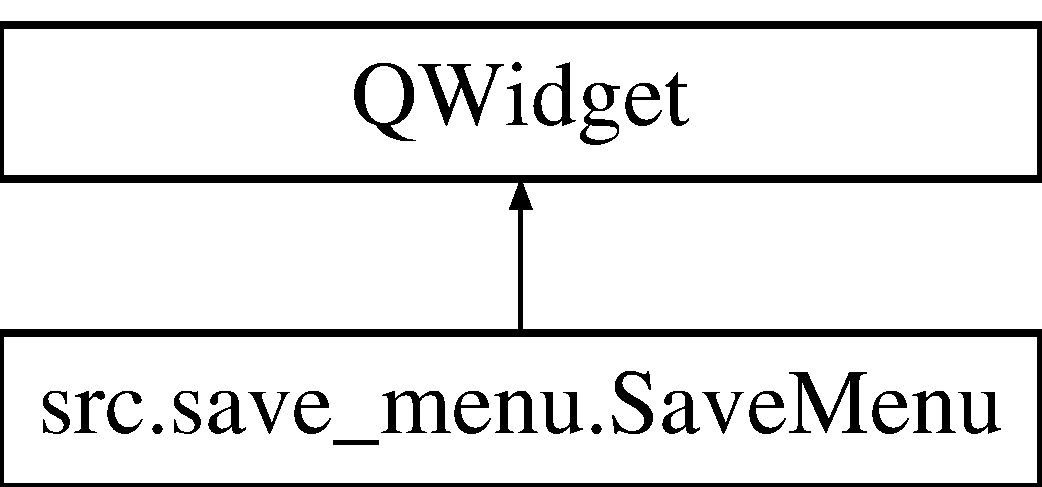
\includegraphics[height=2.000000cm]{classsrc_1_1save__menu_1_1_save_menu}
\end{center}
\end{figure}
\subsection*{Public Member Functions}
\begin{DoxyCompactItemize}
\item 
\hypertarget{classsrc_1_1save__menu_1_1_save_menu_aec50d1d33e455ba8ea30063059ba3270}{}def {\bfseries \+\_\+\+\_\+init\+\_\+\+\_\+}\label{classsrc_1_1save__menu_1_1_save_menu_aec50d1d33e455ba8ea30063059ba3270}

\item 
def \hyperlink{classsrc_1_1save__menu_1_1_save_menu_a69135ce0e32c0ec25e23f4cea0a0eae8}{init\+U\+I} (self)
\begin{DoxyCompactList}\small\item\em this method initialize the G\+U\+I of the save menu. \end{DoxyCompactList}\item 
def \hyperlink{classsrc_1_1save__menu_1_1_save_menu_a318487ca9ed34963dd572faa1ce09c56}{save\+Game} (self)
\begin{DoxyCompactList}\small\item\em this method saves the current game by calling the database method \hyperlink{classsrc_1_1save__menu_1_1_save_menu_a318487ca9ed34963dd572faa1ce09c56}{save\+Game()}. \end{DoxyCompactList}\item 
def \hyperlink{classsrc_1_1save__menu_1_1_save_menu_a91e3ce3f4563456db3102294459a8c43}{return\+To\+Pause\+Menu} (self)
\begin{DoxyCompactList}\small\item\em this method emit return\+To\+Pause\+Menu\+Signal when called. \end{DoxyCompactList}\end{DoxyCompactItemize}
\subsection*{Public Attributes}
\begin{DoxyCompactItemize}
\item 
\hyperlink{classsrc_1_1save__menu_1_1_save_menu_a5d5d8515ced22884dcd1a7f5d1943566}{board}
\begin{DoxyCompactList}\small\item\em is a copy of the current board to be saved. \end{DoxyCompactList}\item 
\hyperlink{classsrc_1_1save__menu_1_1_save_menu_afa694276e009bcb004df7c7a1a5da217}{username}
\begin{DoxyCompactList}\small\item\em is the currently active user\textquotesingle{}s username. \end{DoxyCompactList}\item 
\hyperlink{classsrc_1_1save__menu_1_1_save_menu_aed6ba9a74fc14066593c5ce7b2ae4691}{save\+Label}
\begin{DoxyCompactList}\small\item\em is a Q\+Label that displays \textquotesingle{}Game name\textquotesingle{}. \end{DoxyCompactList}\item 
\hyperlink{classsrc_1_1save__menu_1_1_save_menu_a0673d06683a2c9f326d36958fe339a2a}{game\+Title}
\begin{DoxyCompactList}\small\item\em is a Q\+Line\+Edit that let the user enter the name of the game to be saved. \end{DoxyCompactList}\end{DoxyCompactItemize}
\subsection*{Static Public Attributes}
\begin{DoxyCompactItemize}
\item 
tuple \hyperlink{classsrc_1_1save__menu_1_1_save_menu_a91e3384b3ca4264682fd7cc2fce47b0f}{return\+To\+Pause\+Menu\+Signal} = Qt\+Core.\+pyqt\+Signal()
\begin{DoxyCompactList}\small\item\em Signal which will be used to return to the pause menu. \end{DoxyCompactList}\end{DoxyCompactItemize}


\subsection{Detailed Description}
this class is a widget that displays the save menu. 

It includes the following buttons and fields that the user can interact with\+:~\newline
save\+Button\+: calls \hyperlink{classsrc_1_1save__menu_1_1_save_menu_a318487ca9ed34963dd572faa1ce09c56}{save\+Game()} when clicked.~\newline
return\+Button\+: emit return\+To\+Pause\+Menu\+Signal when clicked. 

\subsection{Member Function Documentation}
\hypertarget{classsrc_1_1save__menu_1_1_save_menu_a69135ce0e32c0ec25e23f4cea0a0eae8}{}\index{src\+::save\+\_\+menu\+::\+Save\+Menu@{src\+::save\+\_\+menu\+::\+Save\+Menu}!init\+U\+I@{init\+U\+I}}
\index{init\+U\+I@{init\+U\+I}!src\+::save\+\_\+menu\+::\+Save\+Menu@{src\+::save\+\_\+menu\+::\+Save\+Menu}}
\subsubsection[{init\+U\+I}]{\setlength{\rightskip}{0pt plus 5cm}def src.\+save\+\_\+menu.\+Save\+Menu.\+init\+U\+I (
\begin{DoxyParamCaption}
\item[{}]{self}
\end{DoxyParamCaption}
)}\label{classsrc_1_1save__menu_1_1_save_menu_a69135ce0e32c0ec25e23f4cea0a0eae8}


this method initialize the G\+U\+I of the save menu. 

\hypertarget{classsrc_1_1save__menu_1_1_save_menu_a91e3ce3f4563456db3102294459a8c43}{}\index{src\+::save\+\_\+menu\+::\+Save\+Menu@{src\+::save\+\_\+menu\+::\+Save\+Menu}!return\+To\+Pause\+Menu@{return\+To\+Pause\+Menu}}
\index{return\+To\+Pause\+Menu@{return\+To\+Pause\+Menu}!src\+::save\+\_\+menu\+::\+Save\+Menu@{src\+::save\+\_\+menu\+::\+Save\+Menu}}
\subsubsection[{return\+To\+Pause\+Menu}]{\setlength{\rightskip}{0pt plus 5cm}def src.\+save\+\_\+menu.\+Save\+Menu.\+return\+To\+Pause\+Menu (
\begin{DoxyParamCaption}
\item[{}]{self}
\end{DoxyParamCaption}
)}\label{classsrc_1_1save__menu_1_1_save_menu_a91e3ce3f4563456db3102294459a8c43}


this method emit return\+To\+Pause\+Menu\+Signal when called. 

\hypertarget{classsrc_1_1save__menu_1_1_save_menu_a318487ca9ed34963dd572faa1ce09c56}{}\index{src\+::save\+\_\+menu\+::\+Save\+Menu@{src\+::save\+\_\+menu\+::\+Save\+Menu}!save\+Game@{save\+Game}}
\index{save\+Game@{save\+Game}!src\+::save\+\_\+menu\+::\+Save\+Menu@{src\+::save\+\_\+menu\+::\+Save\+Menu}}
\subsubsection[{save\+Game}]{\setlength{\rightskip}{0pt plus 5cm}def src.\+save\+\_\+menu.\+Save\+Menu.\+save\+Game (
\begin{DoxyParamCaption}
\item[{}]{self}
\end{DoxyParamCaption}
)}\label{classsrc_1_1save__menu_1_1_save_menu_a318487ca9ed34963dd572faa1ce09c56}


this method saves the current game by calling the database method \hyperlink{classsrc_1_1save__menu_1_1_save_menu_a318487ca9ed34963dd572faa1ce09c56}{save\+Game()}. 



\subsection{Member Data Documentation}
\hypertarget{classsrc_1_1save__menu_1_1_save_menu_a5d5d8515ced22884dcd1a7f5d1943566}{}\index{src\+::save\+\_\+menu\+::\+Save\+Menu@{src\+::save\+\_\+menu\+::\+Save\+Menu}!board@{board}}
\index{board@{board}!src\+::save\+\_\+menu\+::\+Save\+Menu@{src\+::save\+\_\+menu\+::\+Save\+Menu}}
\subsubsection[{board}]{\setlength{\rightskip}{0pt plus 5cm}src.\+save\+\_\+menu.\+Save\+Menu.\+board}\label{classsrc_1_1save__menu_1_1_save_menu_a5d5d8515ced22884dcd1a7f5d1943566}


is a copy of the current board to be saved. 

\hypertarget{classsrc_1_1save__menu_1_1_save_menu_a0673d06683a2c9f326d36958fe339a2a}{}\index{src\+::save\+\_\+menu\+::\+Save\+Menu@{src\+::save\+\_\+menu\+::\+Save\+Menu}!game\+Title@{game\+Title}}
\index{game\+Title@{game\+Title}!src\+::save\+\_\+menu\+::\+Save\+Menu@{src\+::save\+\_\+menu\+::\+Save\+Menu}}
\subsubsection[{game\+Title}]{\setlength{\rightskip}{0pt plus 5cm}src.\+save\+\_\+menu.\+Save\+Menu.\+game\+Title}\label{classsrc_1_1save__menu_1_1_save_menu_a0673d06683a2c9f326d36958fe339a2a}


is a Q\+Line\+Edit that let the user enter the name of the game to be saved. 

\hypertarget{classsrc_1_1save__menu_1_1_save_menu_a91e3384b3ca4264682fd7cc2fce47b0f}{}\index{src\+::save\+\_\+menu\+::\+Save\+Menu@{src\+::save\+\_\+menu\+::\+Save\+Menu}!return\+To\+Pause\+Menu\+Signal@{return\+To\+Pause\+Menu\+Signal}}
\index{return\+To\+Pause\+Menu\+Signal@{return\+To\+Pause\+Menu\+Signal}!src\+::save\+\_\+menu\+::\+Save\+Menu@{src\+::save\+\_\+menu\+::\+Save\+Menu}}
\subsubsection[{return\+To\+Pause\+Menu\+Signal}]{\setlength{\rightskip}{0pt plus 5cm}tuple src.\+save\+\_\+menu.\+Save\+Menu.\+return\+To\+Pause\+Menu\+Signal = Qt\+Core.\+pyqt\+Signal()\hspace{0.3cm}{\ttfamily [static]}}\label{classsrc_1_1save__menu_1_1_save_menu_a91e3384b3ca4264682fd7cc2fce47b0f}


Signal which will be used to return to the pause menu. 

\hypertarget{classsrc_1_1save__menu_1_1_save_menu_aed6ba9a74fc14066593c5ce7b2ae4691}{}\index{src\+::save\+\_\+menu\+::\+Save\+Menu@{src\+::save\+\_\+menu\+::\+Save\+Menu}!save\+Label@{save\+Label}}
\index{save\+Label@{save\+Label}!src\+::save\+\_\+menu\+::\+Save\+Menu@{src\+::save\+\_\+menu\+::\+Save\+Menu}}
\subsubsection[{save\+Label}]{\setlength{\rightskip}{0pt plus 5cm}src.\+save\+\_\+menu.\+Save\+Menu.\+save\+Label}\label{classsrc_1_1save__menu_1_1_save_menu_aed6ba9a74fc14066593c5ce7b2ae4691}


is a Q\+Label that displays \textquotesingle{}Game name\textquotesingle{}. 

\hypertarget{classsrc_1_1save__menu_1_1_save_menu_afa694276e009bcb004df7c7a1a5da217}{}\index{src\+::save\+\_\+menu\+::\+Save\+Menu@{src\+::save\+\_\+menu\+::\+Save\+Menu}!username@{username}}
\index{username@{username}!src\+::save\+\_\+menu\+::\+Save\+Menu@{src\+::save\+\_\+menu\+::\+Save\+Menu}}
\subsubsection[{username}]{\setlength{\rightskip}{0pt plus 5cm}src.\+save\+\_\+menu.\+Save\+Menu.\+username}\label{classsrc_1_1save__menu_1_1_save_menu_afa694276e009bcb004df7c7a1a5da217}


is the currently active user\textquotesingle{}s username. 



The documentation for this class was generated from the following file\+:\begin{DoxyCompactItemize}
\item 
src/save\+\_\+menu.\+py\end{DoxyCompactItemize}

\hypertarget{classsrc_1_1board_1_1_status_bar}{}\section{src.\+board.\+Status\+Bar Class Reference}
\label{classsrc_1_1board_1_1_status_bar}\index{src.\+board.\+Status\+Bar@{src.\+board.\+Status\+Bar}}


This class is a widget which displays the game information while playing.  


Inheritance diagram for src.\+board.\+Status\+Bar\+:\begin{figure}[H]
\begin{center}
\leavevmode
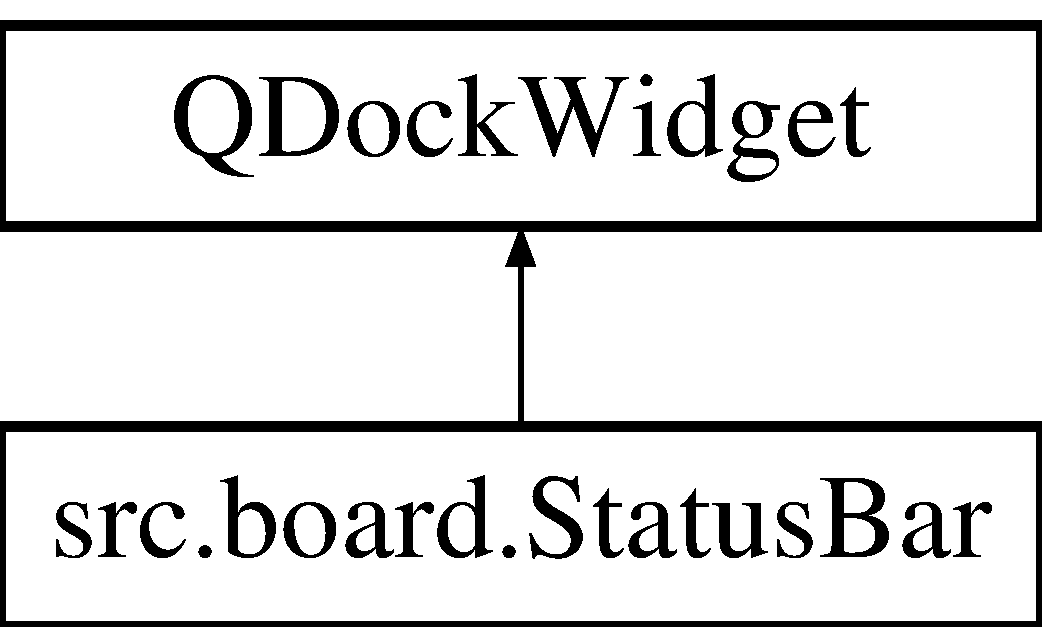
\includegraphics[height=2.000000cm]{classsrc_1_1board_1_1_status_bar}
\end{center}
\end{figure}
\subsection*{Public Member Functions}
\begin{DoxyCompactItemize}
\item 
\hypertarget{classsrc_1_1board_1_1_status_bar_a1f6a41d63501b4eb012a19c243b2cc5b}{}def {\bfseries \+\_\+\+\_\+init\+\_\+\+\_\+}\label{classsrc_1_1board_1_1_status_bar_a1f6a41d63501b4eb012a19c243b2cc5b}

\end{DoxyCompactItemize}
\subsection*{Public Attributes}
\begin{DoxyCompactItemize}
\item 
\hypertarget{classsrc_1_1board_1_1_status_bar_ad91d18f7e226872ae73eef0d347ee5d0}{}{\bfseries lives\+Label}\label{classsrc_1_1board_1_1_status_bar_ad91d18f7e226872ae73eef0d347ee5d0}

\item 
\hypertarget{classsrc_1_1board_1_1_status_bar_a3055230ea568f64edd37decdc4c6dee9}{}{\bfseries times\+Label}\label{classsrc_1_1board_1_1_status_bar_a3055230ea568f64edd37decdc4c6dee9}

\item 
\hypertarget{classsrc_1_1board_1_1_status_bar_a56605adb92e53a3cb03a73c1bb6ada29}{}{\bfseries score\+Label}\label{classsrc_1_1board_1_1_status_bar_a56605adb92e53a3cb03a73c1bb6ada29}

\end{DoxyCompactItemize}


\subsection{Detailed Description}
This class is a widget which displays the game information while playing. 

It includes the following labels\+: lives\+Label\+: Displays number of remaining lives. times\+Label\+: Displays time left. score\+Label\+: Displays the player\textquotesingle{}s score. 

The documentation for this class was generated from the following file\+:\begin{DoxyCompactItemize}
\item 
src/board.\+py\end{DoxyCompactItemize}

\hypertarget{classsrc_1_1tile_1_1_tile}{}\section{src.\+tile.\+Tile Class Reference}
\label{classsrc_1_1tile_1_1_tile}\index{src.\+tile.\+Tile@{src.\+tile.\+Tile}}
Inheritance diagram for src.\+tile.\+Tile\+:\begin{figure}[H]
\begin{center}
\leavevmode
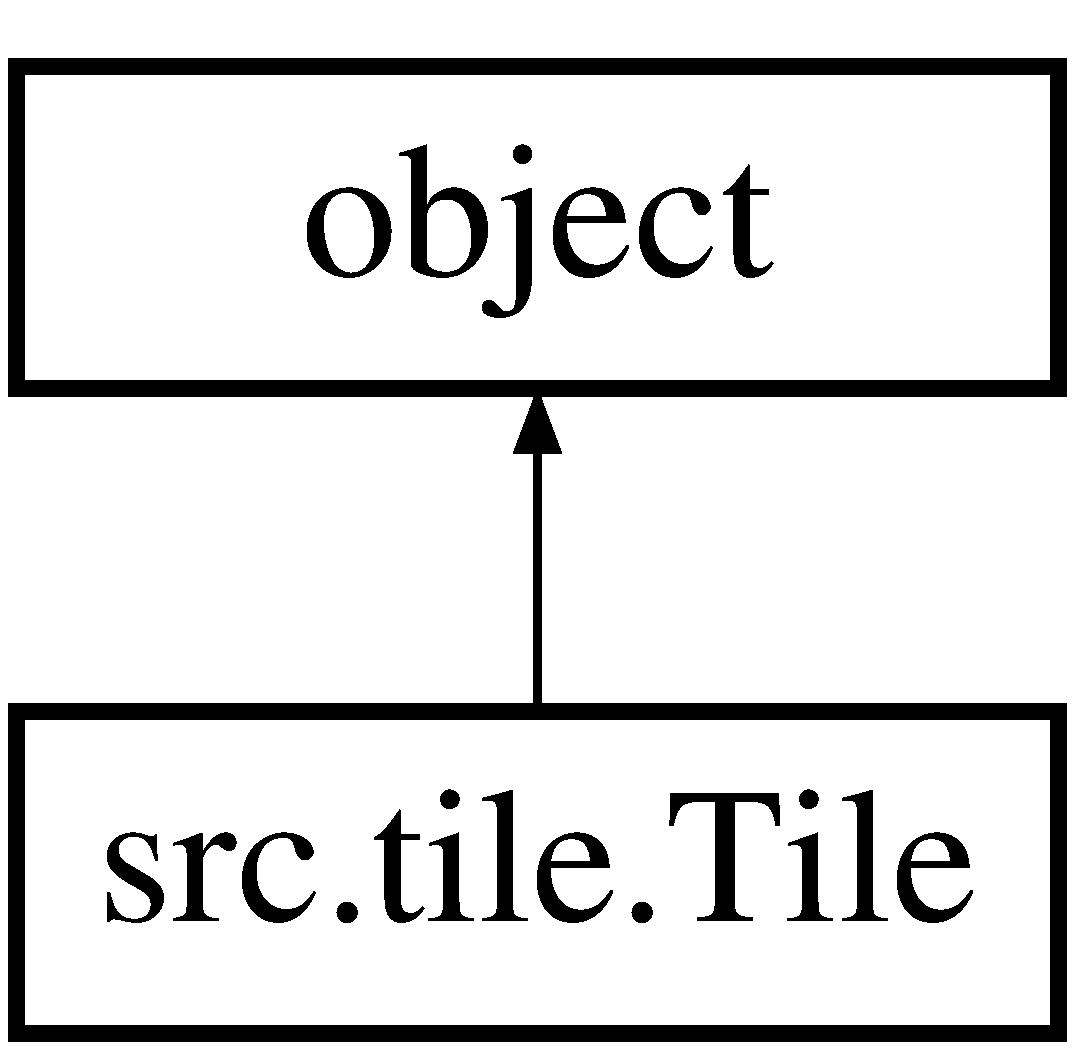
\includegraphics[height=2.000000cm]{classsrc_1_1tile_1_1_tile}
\end{center}
\end{figure}
\subsection*{Public Member Functions}
\begin{DoxyCompactItemize}
\item 
\hypertarget{classsrc_1_1tile_1_1_tile_a9976e652dac509c6aee814af20a6cabb}{}def {\bfseries \+\_\+\+\_\+init\+\_\+\+\_\+} (self)\label{classsrc_1_1tile_1_1_tile_a9976e652dac509c6aee814af20a6cabb}

\item 
\hypertarget{classsrc_1_1tile_1_1_tile_aad77febc9fbb4fa5fd2f13449d1c80da}{}def {\bfseries is\+Empty} (self)\label{classsrc_1_1tile_1_1_tile_aad77febc9fbb4fa5fd2f13449d1c80da}

\item 
\hypertarget{classsrc_1_1tile_1_1_tile_ab682d4a8d92f6dbe5380c21e8c27114a}{}def {\bfseries push} (self, tile)\label{classsrc_1_1tile_1_1_tile_ab682d4a8d92f6dbe5380c21e8c27114a}

\item 
\hypertarget{classsrc_1_1tile_1_1_tile_a0a8402816b245a69773305cc6d86f16d}{}def {\bfseries peek} (self)\label{classsrc_1_1tile_1_1_tile_a0a8402816b245a69773305cc6d86f16d}

\item 
\hypertarget{classsrc_1_1tile_1_1_tile_ae0f31d367515d3259f21b90d6be44db8}{}def {\bfseries pop} (self)\label{classsrc_1_1tile_1_1_tile_ae0f31d367515d3259f21b90d6be44db8}

\item 
\hypertarget{classsrc_1_1tile_1_1_tile_ac9f0ddf090f58449aa74611a239e1458}{}def {\bfseries size} (self)\label{classsrc_1_1tile_1_1_tile_ac9f0ddf090f58449aa74611a239e1458}

\end{DoxyCompactItemize}
\subsection*{Static Public Member Functions}
\begin{DoxyCompactItemize}
\item 
\hypertarget{classsrc_1_1tile_1_1_tile_a402644908c005daf8f452078a8498884}{}def {\bfseries is\+Empty} (tile)\label{classsrc_1_1tile_1_1_tile_a402644908c005daf8f452078a8498884}

\item 
\hypertarget{classsrc_1_1tile_1_1_tile_a26d5b3272e8b49c400420bfb80f2367e}{}def {\bfseries is\+Enemy} (tile)\label{classsrc_1_1tile_1_1_tile_a26d5b3272e8b49c400420bfb80f2367e}

\item 
\hypertarget{classsrc_1_1tile_1_1_tile_abe6a8c872f4e0d314bedb157c5d05f88}{}def {\bfseries is\+Bomberman} (tile)\label{classsrc_1_1tile_1_1_tile_abe6a8c872f4e0d314bedb157c5d05f88}

\item 
\hypertarget{classsrc_1_1tile_1_1_tile_a81e3ba4c45f3defa624c6d5cd080dab6}{}def {\bfseries is\+Exit} (tile)\label{classsrc_1_1tile_1_1_tile_a81e3ba4c45f3defa624c6d5cd080dab6}

\item 
\hypertarget{classsrc_1_1tile_1_1_tile_a464b874776619a4388f7bc8a5a57eee1}{}def {\bfseries is\+Powerup} (tile)\label{classsrc_1_1tile_1_1_tile_a464b874776619a4388f7bc8a5a57eee1}

\end{DoxyCompactItemize}
\subsection*{Public Attributes}
\begin{DoxyCompactItemize}
\item 
\hypertarget{classsrc_1_1tile_1_1_tile_aaad193d1f0e1a1e90570e6069f65b330}{}{\bfseries stack}\label{classsrc_1_1tile_1_1_tile_aaad193d1f0e1a1e90570e6069f65b330}

\end{DoxyCompactItemize}
\subsection*{Static Public Attributes}
\begin{DoxyCompactItemize}
\item 
\hypertarget{classsrc_1_1tile_1_1_tile_a2e2fc149a0f255ddd6a2cd64bf060e04}{}int {\bfseries Empty} = 0\label{classsrc_1_1tile_1_1_tile_a2e2fc149a0f255ddd6a2cd64bf060e04}

\item 
\hypertarget{classsrc_1_1tile_1_1_tile_a7bbfca724a7080f281ccf31fd324182d}{}int {\bfseries Concrete} = 1\label{classsrc_1_1tile_1_1_tile_a7bbfca724a7080f281ccf31fd324182d}

\item 
\hypertarget{classsrc_1_1tile_1_1_tile_ae4e13878d3a81fd1209fac1884f22569}{}int {\bfseries Brick} = 2\label{classsrc_1_1tile_1_1_tile_ae4e13878d3a81fd1209fac1884f22569}

\item 
\hypertarget{classsrc_1_1tile_1_1_tile_a22cc10d99f8785119477645d6e15f1ac}{}int {\bfseries Bomb} = 3\label{classsrc_1_1tile_1_1_tile_a22cc10d99f8785119477645d6e15f1ac}

\item 
\hypertarget{classsrc_1_1tile_1_1_tile_a44a3a6a3a1ed1c80a766b4a971a882af}{}int {\bfseries Bomberman} = 4\label{classsrc_1_1tile_1_1_tile_a44a3a6a3a1ed1c80a766b4a971a882af}

\item 
\hypertarget{classsrc_1_1tile_1_1_tile_afff8f8b451056470316105c1950c8049}{}int {\bfseries Powerup} = 5\label{classsrc_1_1tile_1_1_tile_afff8f8b451056470316105c1950c8049}

\item 
\hypertarget{classsrc_1_1tile_1_1_tile_aaa351173f66c9b5b2afe3ed6a79d68eb}{}int {\bfseries Exit} = 6\label{classsrc_1_1tile_1_1_tile_aaa351173f66c9b5b2afe3ed6a79d68eb}

\item 
\hypertarget{classsrc_1_1tile_1_1_tile_a7b37e5f805d37cd1fa30d999dd4b02cc}{}int {\bfseries Flash} = 7\label{classsrc_1_1tile_1_1_tile_a7b37e5f805d37cd1fa30d999dd4b02cc}

\item 
\hypertarget{classsrc_1_1tile_1_1_tile_a4a2cda5d4e4a662ea9ec19aebd4c75a5}{}int {\bfseries Balloom} = 8\label{classsrc_1_1tile_1_1_tile_a4a2cda5d4e4a662ea9ec19aebd4c75a5}

\item 
\hypertarget{classsrc_1_1tile_1_1_tile_a9b2b4677c74d1d30e93a235d3d997a4a}{}int {\bfseries Oneal} = 9\label{classsrc_1_1tile_1_1_tile_a9b2b4677c74d1d30e93a235d3d997a4a}

\item 
\hypertarget{classsrc_1_1tile_1_1_tile_aeed2c1217d02f0ca8ce5713f28a5543c}{}int {\bfseries Doll} = 10\label{classsrc_1_1tile_1_1_tile_aeed2c1217d02f0ca8ce5713f28a5543c}

\item 
\hypertarget{classsrc_1_1tile_1_1_tile_a5ca9bdbdf6863d2602f3f52adb749125}{}int {\bfseries Minvo} = 11\label{classsrc_1_1tile_1_1_tile_a5ca9bdbdf6863d2602f3f52adb749125}

\item 
\hypertarget{classsrc_1_1tile_1_1_tile_a7d7c123ec8ee03dc3b742828f9ee8690}{}int {\bfseries Kondoria} = 12\label{classsrc_1_1tile_1_1_tile_a7d7c123ec8ee03dc3b742828f9ee8690}

\item 
\hypertarget{classsrc_1_1tile_1_1_tile_a1de207d2b99c4d5978448b3e18e6ceef}{}int {\bfseries Ovapi} = 13\label{classsrc_1_1tile_1_1_tile_a1de207d2b99c4d5978448b3e18e6ceef}

\item 
\hypertarget{classsrc_1_1tile_1_1_tile_ac9fd73aea6f5bd2e72b5a76fe7c0045e}{}int {\bfseries Pass} = 14\label{classsrc_1_1tile_1_1_tile_ac9fd73aea6f5bd2e72b5a76fe7c0045e}

\item 
\hypertarget{classsrc_1_1tile_1_1_tile_a63e8749a3f0bca1c933dc2213ad519ba}{}int {\bfseries Pontan} = 15\label{classsrc_1_1tile_1_1_tile_a63e8749a3f0bca1c933dc2213ad519ba}

\end{DoxyCompactItemize}


The documentation for this class was generated from the following file\+:\begin{DoxyCompactItemize}
\item 
src/tile.\+py\end{DoxyCompactItemize}

\hypertarget{classsrc_1_1models_1_1_user_account}{}\section{src.\+models.\+User\+Account Class Reference}
\label{classsrc_1_1models_1_1_user_account}\index{src.\+models.\+User\+Account@{src.\+models.\+User\+Account}}


Instances of this class represent all information relevant to a specific user account.  


\subsection*{Public Member Functions}
\begin{DoxyCompactItemize}
\item 
def \hyperlink{classsrc_1_1models_1_1_user_account_a027838850b725021534e05b2efffdc8f}{\+\_\+\+\_\+init\+\_\+\+\_\+} (self, username, realname, password, max\+Level\+Reached=1, cumulative\+Score=0, num\+Games\+Played=0)
\begin{DoxyCompactList}\small\item\em Constructor with three required parameters\+: username, realname, and password. \end{DoxyCompactList}\end{DoxyCompactItemize}
\subsection*{Public Attributes}
\begin{DoxyCompactItemize}
\item 
\hypertarget{classsrc_1_1models_1_1_user_account_a324ce15e04522bc6d7e1b1518f7a9810}{}{\bfseries username}\label{classsrc_1_1models_1_1_user_account_a324ce15e04522bc6d7e1b1518f7a9810}

\item 
\hypertarget{classsrc_1_1models_1_1_user_account_a0fce5f371818dfb89c6837313497dbb5}{}{\bfseries realname}\label{classsrc_1_1models_1_1_user_account_a0fce5f371818dfb89c6837313497dbb5}

\item 
\hypertarget{classsrc_1_1models_1_1_user_account_a94b6fb51043b9cd72661f232aac24168}{}{\bfseries password}\label{classsrc_1_1models_1_1_user_account_a94b6fb51043b9cd72661f232aac24168}

\item 
\hypertarget{classsrc_1_1models_1_1_user_account_ac3bcbebd2526795af0c1be70b8100434}{}{\bfseries max\+Level\+Reached}\label{classsrc_1_1models_1_1_user_account_ac3bcbebd2526795af0c1be70b8100434}

\item 
\hypertarget{classsrc_1_1models_1_1_user_account_aba4c0aff5e1f4aa209fef3a9d77b7bb7}{}{\bfseries cumulative\+Score}\label{classsrc_1_1models_1_1_user_account_aba4c0aff5e1f4aa209fef3a9d77b7bb7}

\item 
\hypertarget{classsrc_1_1models_1_1_user_account_adb4b6601e342d936266c44a9e809e3db}{}{\bfseries num\+Games\+Played}\label{classsrc_1_1models_1_1_user_account_adb4b6601e342d936266c44a9e809e3db}

\end{DoxyCompactItemize}


\subsection{Detailed Description}
Instances of this class represent all information relevant to a specific user account. 

\subsection{Constructor \& Destructor Documentation}
\hypertarget{classsrc_1_1models_1_1_user_account_a027838850b725021534e05b2efffdc8f}{}\index{src\+::models\+::\+User\+Account@{src\+::models\+::\+User\+Account}!\+\_\+\+\_\+init\+\_\+\+\_\+@{\+\_\+\+\_\+init\+\_\+\+\_\+}}
\index{\+\_\+\+\_\+init\+\_\+\+\_\+@{\+\_\+\+\_\+init\+\_\+\+\_\+}!src\+::models\+::\+User\+Account@{src\+::models\+::\+User\+Account}}
\subsubsection[{\+\_\+\+\_\+init\+\_\+\+\_\+}]{\setlength{\rightskip}{0pt plus 5cm}def src.\+models.\+User\+Account.\+\_\+\+\_\+init\+\_\+\+\_\+ (
\begin{DoxyParamCaption}
\item[{}]{self, }
\item[{}]{username, }
\item[{}]{realname, }
\item[{}]{password, }
\item[{}]{max\+Level\+Reached = {\ttfamily 1}, }
\item[{}]{cumulative\+Score = {\ttfamily 0}, }
\item[{}]{num\+Games\+Played = {\ttfamily 0}}
\end{DoxyParamCaption}
)}\label{classsrc_1_1models_1_1_user_account_a027838850b725021534e05b2efffdc8f}


Constructor with three required parameters\+: username, realname, and password. 


\begin{DoxyParams}{Parameters}
{\em username} & Required. The username associated to the account. Used as key to retrieve all other fields from the database \\
\hline
{\em realname} & Required. The real name of the user \\
\hline
{\em password} & Required. The password of the user \\
\hline
{\em max\+Level\+Reached} & Default is 1. Used to initialize the user account with a specific unlocked level \\
\hline
{\em cumulative\+Score} & Default is 0. Used to initialize the user account with a specific cumulative score \\
\hline
{\em num\+Games\+Played} & Default is 0. Used to initialize the user account with a specific number of games played \\
\hline
\end{DoxyParams}


The documentation for this class was generated from the following file\+:\begin{DoxyCompactItemize}
\item 
src/models.\+py\end{DoxyCompactItemize}

%--- End generated contents ---

% Index
\backmatter
\newpage
\phantomsection
\clearemptydoublepage
\addcontentsline{toc}{chapter}{Index}
\printindex

\end{document}
